\documentclass[a4paper,10pt]{book}
\usepackage[english]{babel}     
\usepackage[utf8]{inputenc}     % accent symbols
\usepackage[T1]{fontenc}
\usepackage{lmodern}
\usepackage{microtype}
\usepackage{natbib}
\usepackage{tocbibind}          
\usepackage{amsmath}            % math symbols
\usepackage{amsthm}             % math symbols
\usepackage[colorlinks=true,linkcolor=red]{hyperref} % hyper link

% for code
\usepackage{listings}
\usepackage{color,xcolor}
\definecolor{mygreen}{rgb}{0,0.6,0}
\definecolor{mygray}{rgb}{0.9,0.9,0.9}
\definecolor{mymauve}{rgb}{0.58,0,0.82}
\lstset{
backgroundcolor=\color{mygray},
numbers=left,                    
columns=fullflexible,
breaklines=true,      
captionpos=b,         
tabsize=4,            
commentstyle=\color{mygreen}, 
escapeinside={\%*}{*)},       
keywordstyle=\color{blue},    
% stringstyle=\color{mymauve}\monaco,
frame=single,                        
rulesepcolor=\color{red!20!green!20!blue!20},
% identifierstyle=\color{red},
%% language=c++,
basicstyle=\tiny
}

\usepackage{indentfirst}
\setlength{\parindent}{2em}
\usepackage[onehalfspacing]{setspace}
% graph
\usepackage{pdfpages}
\usepackage{graphicx}
% box
\usepackage{booktabs}
\usepackage{tcolorbox}

%% user defined command
\newcommand{\keyword}[1]{\textbf{#1}}
\newcommand{\keywords}[1]{\textbf{#1}}
\newcommand{\lcmd}[1]{\texttt{#1}}
\newcommand{\head}[1]{\textnormal{\textbf{#1}}}
\newcommand{\itwords}[1]{\textit{#1}}

\usepackage{float}
% all symbols
\usepackage{tipa}
\usepackage{tipx}

\usepackage{datetime}
% \usepackage{movie15}


% variable
% TODO
\newcommand{\pdfauthor}{李明明}
\newcommand{\pdftitle}{工作}
\newcommand{\pdfsubject}{工作中的经验与教训}
\newcommand{\pdfkeywords}{工作经验与教训}
\newcommand{\bookname}{工作收获}
\newcommand{\bookoneword}{工作中吸取的经验和教训}
\newcommand{\timeandcompany}{2020年12月1日}

\usepackage{bm}
\usepackage{amsfonts}
\begin{document}

\newcommand{\mytitle}{Git}
\newcommand{\firstcreated}{Mar 16, 2023}

\begin{titlepage}

\newcommand{\HRule}{\rule{\linewidth}{0.5mm}} % Defines a new command for the horizontal lines, change thickness here

\center                         % Center everything on the page
 
%----------------------------------------------------------------------------------------
%	HEADING SECTIONS
%----------------------------------------------------------------------------------------


\includegraphics[width=0.5\textwidth]{logo}\\[1cm] % Include a department/university logo - this will require the graphicx package

%----------------------------------------------------------------------------------------
%	TITLE SECTION
%----------------------------------------------------------------------------------------

\HRule\\[0.4cm]
{ \huge \bfseries \mytitle}\\[0.4cm] % Title of your document
\HRule\\[1.5cm]
 
%----------------------------------------------------------------------------------------
%	AUTHOR SECTION
%----------------------------------------------------------------------------------------

\begin{minipage}{0.4\textwidth}
\begin{center} \large
Mingming \textsc{Li}\\ % Your name
\end{center}

\end{minipage}\\[2cm]


%----------------------------------------------------------------------------------------
%	DATE SECTION
% ----------------------------------------------------------------------------------------
\vfill
{\large First Created: \firstcreated}\\
{\large Last Modified: \today}\\[2cm] % Date, change the \today to a set date if you want to be precise



\end{titlepage}


%%% Local Variables:
%%% mode: latex
%%% Tex-master: "git"
%%% End:

% Pages are numbered with lowercase Roman numbers.
% Chapters generate a table of contents entry but don't get a number.
\frontmatter

\tableofcontents{}
\listoffigures{}
\listoftables{}

% Pages are numbered with Arabic numbers.
% Chapters are numbered and produce a table of contents entry.
\mainmatter 


\chapter{\LaTeX\xspace Base}


\section{What is \LaTeX}
\label{sec:what-latex}

\LaTeX\index{latex} is a document markup language\footnote{Just like HTML}. It separate format from content.

\section{Reason to Use It}


Because \LaTeX \xspace{} is a markup language, you should learn it before you can use it.
So why should you spend so much time to learn it while there is so much document creator like Word, Pages?

There is several reasons that push me to select it.
\begin{itemize}
\item It provides powerful edit ability. You can almost get whatever you want to show, especially the mathematical equations.
\item Because it separate the format and the content, it is easy to do format alteration in the full document domain.
\item Once you create your own template, it is easy to wreate document with the template applied, saving so much time in format. 
\end{itemize}



\section{Logical formatting}
\index{latex!{logical formatting}}
\lstset{language=TeX}
\begin{lstlisting}
  \documentclass{article}
  \begin{document}
  \title{Example}
  \author{Mingming Li}
  \date{2022/11/04}
  \maketitle{}
  \section{Logical Formatting}
  This example show logical formatting.
  \end{document}
\end{lstlisting}

We do not specify the font family, font size, and so on, instead we tell \LaTeX \ the \keyword{class}, the \keyword{author}, or the \keyword{section} and let \LaTeX{} to format it.



\section{Command}
\index{latex!command}
LaTeX commands begin with a backslash, followed by big or small letters.
LaTeX commands are usually named with small letters and in a descriptive way.
There are exceptions: a backslash and just one special character.
Commands may have arguments, given in curly braces or in square brackets.

Calling a command looks like the following:


\begin{lstlisting}
  \command
  \command{argument}
  \command[optional argument]{argument}
\end{lstlisting}

For example

\begin{lstlisting}
  {\large Title}
  \usepackage[english]{babel}     
\usepackage[utf8]{inputenc}     % accent symbols
\usepackage[T1]{fontenc}
\usepackage{lmodern}
\usepackage{microtype}
\usepackage{natbib}
\usepackage{tocbibind}          
\usepackage{amsmath}            % math symbols
\usepackage{amsthm}             % math symbols
\usepackage[colorlinks=true,linkcolor=red]{hyperref} % hyper link

% for code
\usepackage{listings}
\usepackage{color,xcolor}
\definecolor{mygreen}{rgb}{0,0.6,0}
\definecolor{mygray}{rgb}{0.9,0.9,0.9}
\definecolor{mymauve}{rgb}{0.58,0,0.82}
\lstset{
backgroundcolor=\color{mygray},
numbers=left,                    
columns=fullflexible,
breaklines=true,      
captionpos=b,         
tabsize=4,            
commentstyle=\color{mygreen}, 
escapeinside={\%*}{*)},       
keywordstyle=\color{blue},    
% stringstyle=\color{mymauve}\monaco,
frame=single,                        
rulesepcolor=\color{red!20!green!20!blue!20},
% identifierstyle=\color{red},
%% language=c++,
basicstyle=\tiny
}

\usepackage{indentfirst}
\setlength{\parindent}{2em}
\usepackage[onehalfspacing]{setspace}
% graph
\usepackage{pdfpages}
\usepackage{graphicx}
% box
\usepackage{booktabs}
\usepackage{tcolorbox}

%% user defined command
\newcommand{\keyword}[1]{\textbf{#1}}
\newcommand{\keywords}[1]{\textbf{#1}}
\newcommand{\lcmd}[1]{\texttt{#1}}
\newcommand{\head}[1]{\textnormal{\textbf{#1}}}
\newcommand{\itwords}[1]{\textit{#1}}

\usepackage{float}
% all symbols
\usepackage{tipa}
\usepackage{tipx}

\usepackage{datetime}
% \usepackage{movie15}


% variable
% TODO
\newcommand{\pdfauthor}{李明明}
\newcommand{\pdftitle}{工作}
\newcommand{\pdfsubject}{工作中的经验与教训}
\newcommand{\pdfkeywords}{工作经验与教训}
\newcommand{\bookname}{工作收获}
\newcommand{\bookoneword}{工作中吸取的经验和教训}
\newcommand{\timeandcompany}{2020年12月1日}

\usepackage{bm}
\usepackage{amsfonts}
  \documentclass[12pt]{article}
\end{lstlisting}

\section{Comment}
\index{latex!comment}
The percent sing(\%) introduces a \keyword{comment}.


\begin{lstlisting}
  \usepackage[english]{babel}     
\usepackage[utf8]{inputenc}     % accent symbols
\usepackage[T1]{fontenc}
\usepackage{lmodern}
\usepackage{microtype}
\usepackage{natbib}
\usepackage{tocbibind}          
\usepackage{amsmath}            % math symbols
\usepackage{amsthm}             % math symbols
\usepackage[colorlinks=true,linkcolor=red]{hyperref} % hyper link

% for code
\usepackage{listings}
\usepackage{color,xcolor}
\definecolor{mygreen}{rgb}{0,0.6,0}
\definecolor{mygray}{rgb}{0.9,0.9,0.9}
\definecolor{mymauve}{rgb}{0.58,0,0.82}
\lstset{
backgroundcolor=\color{mygray},
numbers=left,                    
columns=fullflexible,
breaklines=true,      
captionpos=b,         
tabsize=4,            
commentstyle=\color{mygreen}, 
escapeinside={\%*}{*)},       
keywordstyle=\color{blue},    
% stringstyle=\color{mymauve}\monaco,
frame=single,                        
rulesepcolor=\color{red!20!green!20!blue!20},
% identifierstyle=\color{red},
%% language=c++,
basicstyle=\tiny
}

\usepackage{indentfirst}
\setlength{\parindent}{2em}
\usepackage[onehalfspacing]{setspace}
% graph
\usepackage{pdfpages}
\usepackage{graphicx}
% box
\usepackage{booktabs}
\usepackage{tcolorbox}

%% user defined command
\newcommand{\keyword}[1]{\textbf{#1}}
\newcommand{\keywords}[1]{\textbf{#1}}
\newcommand{\lcmd}[1]{\texttt{#1}}
\newcommand{\head}[1]{\textnormal{\textbf{#1}}}
\newcommand{\itwords}[1]{\textit{#1}}

\usepackage{float}
% all symbols
\usepackage{tipa}
\usepackage{tipx}

\usepackage{datetime}
% \usepackage{movie15}


% variable
% TODO
\newcommand{\pdfauthor}{李明明}
\newcommand{\pdftitle}{工作}
\newcommand{\pdfsubject}{工作中的经验与教训}
\newcommand{\pdfkeywords}{工作经验与教训}
\newcommand{\bookname}{工作收获}
\newcommand{\bookoneword}{工作中吸取的经验和教训}
\newcommand{\timeandcompany}{2020年12月1日}

\usepackage{bm}
\usepackage{amsfonts}  % include preamble tex file
\end{lstlisting}

\section{Environment}
\label{sec:environment}
\index{latex!environment}
\begin{lstlisting}
  % This is the environment syntax.
  \begin{name}[optional argument]{argument}
    ...
  \end{name}
\end{lstlisting}


\section{Breaks and Empty Lines}
\label{sec:breaks-empty-lines}

LaTeX treats multiple spaces just like a single space.
Also, a single line break has the same effect like a single space.
It doesn't matter how you arrange your text in the editor using spaces or breaks, the output will stay the same.
A blank line denotes a paragraph break.
Like spaces, multiple empty lines are treated as one.
Briefly said, spaces separate words, empty lines separate paragraphs.


\section{Special Symbols}
\label{sec:special-symbols}
\index{latex!symbols}
By putting a backslash before such a special symbol, we turned it into a LaTeX command.
This command has the only purpose of printing out that symbol.



\begin{lstlisting}
  \%  % just print % symbol
  \textbackslash % just print \ symbol
\end{lstlisting}




\section{Create Your Own Commands}

\begin{lstlisting}
  % This is the full definition of creating you own command.
  \newcommand{command}[arguments][optional]{definition}
\end{lstlisting}


\begin{lstlisting}
  % With no arguments.
  \newcommand{\TUG}{TeX Users Group\xspace}
  \TUG

  % With arguments.
  \newcommand{\keyword}[1]{\textbf{#1}}
  \keyword{declrations}

  % With optional arguments.
  \newcommand{\keyword2}[2][\bfseries]{{#1#2}}
  \keyword2[\itshape]{declarations}
\end{lstlisting}


\section{Get Help}
Three ways to get help about the package:
\begin{enumerate}
  
\item 
\begin{lstlisting}[language=sh]
    texdoc <package>
\end{lstlisting}

\item
\begin{lstlisting}[language=sh]
    kpsewhich <package>.sty
\end{lstlisting}

\item Visit the website: \url{http://ctan.org/pkg}

\end{enumerate}

\section{Install Extra Packages}
\label{sec:inst-extra-pack}

The easy way is to use the terminal to install extra packages:

\begin{lstlisting}[language=sh]
# Tex Live manager
tlmgr install <package>
\end{lstlisting}




\section{Floats}
\index{latex!float}


\LaTeX\xspace provides two floating environments, namely,
\argument{figure} and \argument{table}. They are briefly called
\keyword{floats}. Their content may float to a place where it's the
optimum for the page layout.


Here's the float placement options:
\begin{itemize}
\item h: here. The float may appear where it's been written in the source code.
\item t: top. Placing at the top of a page is permitted.
\item b: bottom. The float may appear at the bottom of a page.
\item p: page. The float is allowed to appear on a separate page,
  where only floats may reside but no normal text.
\item !: tells LaTeX to try harder! Some constraints may be ignored,
  easing the placement.
\end{itemize}


The most flexible is using the placement \argument{[!htbp]}, allowing a float
everywhere.







\section{Modes}
\label{sec:modes}

LaTeX knows three general \keyword{modes}:
\begin{itemize}
\item The \keyword{paragraph mode}: The text is typeset as a sequence of words in lines, paragraphs, and pages.
\item The \keyword{left-to-right mode}: The text is also considered to be a sequence of words, but LaTeX typesets it from left to right without breaking the line. 
\item The \keyword{math mode}: Letters are treated as math symbols. A lot of symbols can be used, most of them exclusively in this mode. Such symbols are roots, sum signs, relation signs, math accents, arrows, and various delimiters like brackets and braces. Space characters between letters and symbols are ignored. 
\end{itemize}



%%% Local Variables:
%%% mode: latex
%%% TeX-master: "latex"
%%% End:

\documentclass[a4paper,10pt]{book}
\usepackage[english]{babel}     
\usepackage[utf8]{inputenc}     % accent symbols
\usepackage[T1]{fontenc}
\usepackage{lmodern}
\usepackage{microtype}
\usepackage{natbib}
\usepackage{tocbibind}          
\usepackage{amsmath}            % math symbols
\usepackage{amsthm}             % math symbols
\usepackage[colorlinks=true,linkcolor=red]{hyperref} % hyper link

% for code
\usepackage{listings}
\usepackage{color,xcolor}
\definecolor{mygreen}{rgb}{0,0.6,0}
\definecolor{mygray}{rgb}{0.9,0.9,0.9}
\definecolor{mymauve}{rgb}{0.58,0,0.82}
\lstset{
backgroundcolor=\color{mygray},
numbers=left,                    
columns=fullflexible,
breaklines=true,      
captionpos=b,         
tabsize=4,            
commentstyle=\color{mygreen}, 
escapeinside={\%*}{*)},       
keywordstyle=\color{blue},    
% stringstyle=\color{mymauve}\monaco,
frame=single,                        
rulesepcolor=\color{red!20!green!20!blue!20},
% identifierstyle=\color{red},
%% language=c++,
basicstyle=\tiny
}

\usepackage{indentfirst}
\setlength{\parindent}{2em}
\usepackage[onehalfspacing]{setspace}
% graph
\usepackage{pdfpages}
\usepackage{graphicx}
% box
\usepackage{booktabs}
\usepackage{tcolorbox}

%% user defined command
\newcommand{\keyword}[1]{\textbf{#1}}
\newcommand{\keywords}[1]{\textbf{#1}}
\newcommand{\lcmd}[1]{\texttt{#1}}
\newcommand{\head}[1]{\textnormal{\textbf{#1}}}
\newcommand{\itwords}[1]{\textit{#1}}

\usepackage{float}
% all symbols
\usepackage{tipa}
\usepackage{tipx}

\usepackage{datetime}
% \usepackage{movie15}


% variable
% TODO
\newcommand{\pdfauthor}{李明明}
\newcommand{\pdftitle}{工作}
\newcommand{\pdfsubject}{工作中的经验与教训}
\newcommand{\pdfkeywords}{工作经验与教训}
\newcommand{\bookname}{工作收获}
\newcommand{\bookoneword}{工作中吸取的经验和教训}
\newcommand{\timeandcompany}{2020年12月1日}

\usepackage{bm}
\usepackage{amsfonts}
\begin{document}


% Pages are numbered with lowercase Roman numbers.
% Chapters generate a table of contents entry but don't get a number.
\frontmatter{}
\newcommand{\mytitle}{Git}
\newcommand{\firstcreated}{Mar 16, 2023}

\begin{titlepage}

\newcommand{\HRule}{\rule{\linewidth}{0.5mm}} % Defines a new command for the horizontal lines, change thickness here

\center                         % Center everything on the page
 
%----------------------------------------------------------------------------------------
%	HEADING SECTIONS
%----------------------------------------------------------------------------------------


\includegraphics[width=0.5\textwidth]{logo}\\[1cm] % Include a department/university logo - this will require the graphicx package

%----------------------------------------------------------------------------------------
%	TITLE SECTION
%----------------------------------------------------------------------------------------

\HRule\\[0.4cm]
{ \huge \bfseries \mytitle}\\[0.4cm] % Title of your document
\HRule\\[1.5cm]
 
%----------------------------------------------------------------------------------------
%	AUTHOR SECTION
%----------------------------------------------------------------------------------------

\begin{minipage}{0.4\textwidth}
\begin{center} \large
Mingming \textsc{Li}\\ % Your name
\end{center}

\end{minipage}\\[2cm]


%----------------------------------------------------------------------------------------
%	DATE SECTION
% ----------------------------------------------------------------------------------------
\vfill
{\large First Created: \firstcreated}\\
{\large Last Modified: \today}\\[2cm] % Date, change the \today to a set date if you want to be precise



\end{titlepage}


%%% Local Variables:
%%% mode: latex
%%% Tex-master: "git"
%%% End:
\cleardoublepage{}
\phantomsection{}
\tableofcontents{}
\cleardoublepage{}
\phantomsection{}
\listoffigures{}
\cleardoublepage{}
\phantomsection{}
\listoftables{}


% Pages are numbered with Arabic numbers.
% Chapters are numbered and produce a table of contents entry.
\mainmatter{}
\chapter{Emacs Basics}
\section{What is Emacs?}

Emacs is an text editor.


Learning to use an editor is basically a matter of learning finger habit.
Good finger habits can make you an incredibly fast typist.
Intellectually, it's possible to absorb a lot from one reading, but you can form only a few new habit each day.
Don't feel obliged  to learn them all at once; pick something, practice it, and move on to the next topic.
Time spent developing good habits is time well spent.


\section{Why You Should Use Emacs}
There are following reasons to use Emacs:
\begin{itemize}
\item \keyword{Efficiency}: There are many commands that can move cursor without a mouse. There are many commands to help you saving typing.
\item \keyword{Powerful}: It provides many major and minor modes for special situation. I often use the latex mode.
\item \keyword{Extensibility}: If there is some function not meeting your need, you can programm to implement it using Emacs Lisp language.
\end{itemize}



\section{Files and Buffers}
In Emacs, you don't really edit \keyword{files} (stored on disk).
Instead, Emacs copies the content of a file into a temporary \keyword{buffer} and you edit that.
The file on disk doesn't change until you save the buffer.

\section{Modes}
Emacs becomes sensitive to the task at hand.
\keyword{Modes} allows Emacs to the kind of editor you want for different tasks.
A buffer can be in only one \keyword{major mode} at a time.
\keyword{Minor modes} defines a particular aspect of Emacs's behavior and can be turned on and off within a major mode.

If you are good at Lisp programming, you can add your own modes.
Emacs is almost infinitely extensible.


\section{Display}
\label{sec:display}

The display is shown in Figure \ref{fig:display}.

\begin{figure}[!htbp]
  \centering
  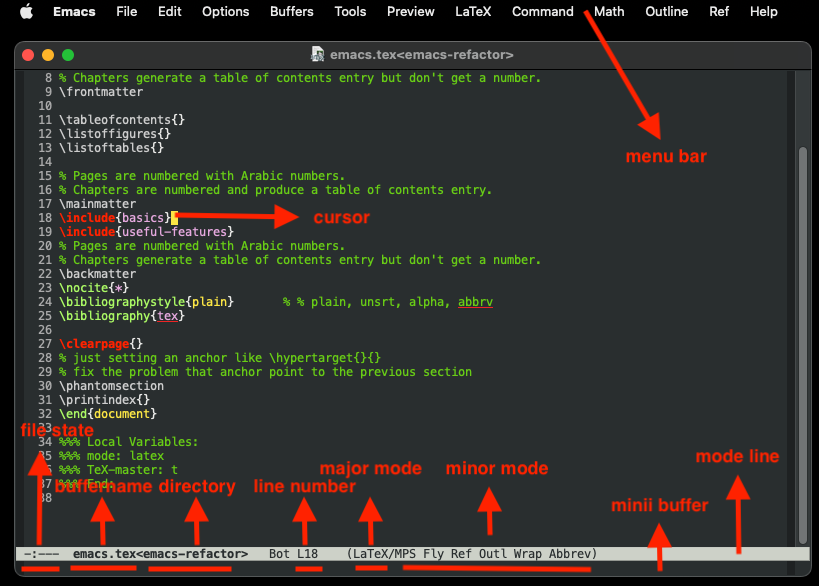
\includegraphics[width=0.9\textwidth]{display}
  \caption{Display}
  \label{fig:display}
\end{figure}


Here I have configured Emacs to hide the tool bar.
The operation is: Options $\longrightarrow$ Show/Hide $\longrightarrow$ Toolbar.
After that, you will see the following file in \argument{~/.emacs}:

\begin{lstlisting}
(custom-set-variables
 '(tool-bar-mode nil))
\end{lstlisting}

The \keyword{mode line} is the place to some useful information.
The \keyword{file state} shows the state of the current buffer.
For example, it is read only or not, altered or not.

\section{Commands}
You issue commands to instruct Emacs to do what you want to.
Each \keyword{command} has a formal name, which is the name of a Lisp routine (Emacs is written with Emacs Lisp language).
Some command names are quite long.
As a result, we need some way to abbreviate commands.
Emacs ties a command name to a short sequence of keystrokes.
This tying of commands to keystrokes is known as \keyword{binding}.


The author of Emacs try to bind the most frequently used commands to the key sequences that are the easiest to reach (\keyword{C: Ctrl, M: Meta}):
\begin{itemize}
\item The most commonly used commands are bound to \keyword{C-n}(where \keyword{n} is any character).
\item Slightly less commonly used commands are bound to \keyword{M-n}.
\item Other commonly used commands are bound to \keyword{C-x keystrokes}.
\item Some specialized commands are bound to \keyword{C-c keystrokes}. These commands often relate to one of the more specialized modes, such as Java or HTML mode.
\item To use commands that is binded, use \keyword{M-x command-name Enter}. (This works for any command really)
\end{itemize}


\section{Kill Ring}
\label{sec:kill-ring}

Emacs use \keyword{kill} commands to delete text, for example \keyword{kill-region, kill-word}.
However, killing is not fatal, but in fact, quite the opposite.
Text that has been killed is not gone forever but is hidden in an area called the \keyword{kill ring}.
The kill ring is an internal storage area where Emacs puts things you’ve copied or deleted.



What exactly goes into the kill ring?
Only the text delete by \keyword{Del} and \keyword{C-d} (without numeric argument) does not go into kill ring. All the else will go into kill ring.


\section{Pointer and Cursor}
\label{sec:pointer-mark}

A \keyword{cursor} is on the top the char.
A \keyword{pointer} is the position between the cursor and one char before the cursor.


\section{Backup Files}
\label{sec:backup-files}

A backup file is a copy of the old contents of a file you are editing.
Emacs makes a backup file the first time you save a buffer into its visited file.
Thus, normally, the backup file contains the contents of the file as it was before the current editing session.
The contents of the backup file normally remain unchanged once it exists.
Thus the backup file keeps a copy of the original file.
During the editing, you may save the buffer several times and the content of the original file will change accordingly.

The name of the backup file is the same as the name of the file you’re editing, with a tilde (\textasciitilde{}) added.
For example, if you are editing the file \argument{text}, the backup file is \argument{text\textasciitilde{}}


\section{Auto Save Files}
\label{sec:auto-save-files}

Emacs will auto save you files from time to time into \argument{auto-save files}.
The name of an auto-save file is the same as the name of the file you are editing, with a sharp (\#) added to the beginning and the end.
For example, if you are editing the file \argument{text}, its auto-save file is \argument{\#text\#}.

The save files are used save the content of current buffer if you do not save the buffer and the Emacs or system crashed.









%%% Local Variables:
%%% mode: latex
%%% TeX-master: "emacs"
%%% End:


\chapter{Start With Emacs}
\label{cha:start-with-emacs}

\section{Start Emacs}
\label{sec:start-emacs}

There are two ways to start Emacs:
\begin{itemize}
\item Click the Emacs icon \parbox{2em}{
\includegraphics[width=2em]{logo}}.
\item Use the command \argument{emacs} in your terminal.
\end{itemize}


\begin{lstlisting}[language=sh]
# To get emacs usage.
emacs --help

# To simply start the Emacs
emacs
\end{lstlisting}


\section{Exit Emacs}
\label{sec:exit-emacs}

In Emacs, use \keyword{C-x C-c} (x: execute; c: clear) to exit.


\section{Working With Files}
\label{sec:working-with-files}

\begin{table}[H]
  \centering
  \begin{tabular}{>{\bfseries}lp{0.5\textwidth}}
    \toprule
    Binding & \head{Meaning}\\
    \midrule
    C-x C-f (f: file)& Open or create a file.\\
    C-x C-v & Read an alternate file, replacing the one read with \keyword{C-x C-f}.\\
    C-x i (i: insert) & Insert file at cursor position.\\
    C-x C-s (s: save) & Save buffer.\\
    C-x C-w (w: write) & Save buffer as another file.\\
    \bottomrule
  \end{tabular}
  \caption{Working with files}
  \label{tab:working-with-files}
\end{table}
%%% Local Variables:
%%% mode: latex
%%% TeX-master: "emacs"
%%% End:


\chapter{Editing}
\label{cha:editing}

\section{Moving Cursor}
\label{sec:moving-cursor}

\begin{table}[H]
  \centering
  \begin{tabular}{l>{\bfseries}lp{0.5\textwidth}}
    \toprule
    \head{Group} & \head{Binding} & \head{Meaning}\\
    \midrule
    \multirow{4}{*}{char} & C-f (f: forward) & forward one char\\
                 & C-b (b: backward) & backward one char\\
                 & C-n (n: next line) & downward one char\\
                 & C-p (p: previous line) & upward one char\\
    \midrule
    \multirow{2}{*}{word} & M-f & forward one word\\
                 & M-b & backward one word\\
    \midrule
    \multirow{2}{*}{line} & C-a & beginning of line\\
                 & C-e & end of line\\
    \midrule
    \multirow{2}{*}{sentence} & M-a & start of sentence\\
                 & M-e & end of sentence\\
    \midrule
    \multirow{2}{*}{paragraph} & M-\{ & start of paragraph\\
                 & M-\} & end of paragraph\\
    \midrule
    \multirow{2}{*}{screen} & C-v & downward one screen\\
                 & M-v & upward one screen\\
                 & C-l & scroll the window so that current line is in the middle of the window, type again, cursor on top, again, bottom\\
                 & C-M-v & scroll other window\\
    \midrule
    \multirow{2}{*}{buffer} & M-< & start of buffer\\
                 & M-> & end of buffer\\
    \midrule
                 & M-m & first non-whitespace character on this line\\
    \midrule
                 & F10 & start key navigation of the menu bar\\
    \bottomrule
  \end{tabular}
  \caption{Moving Cursor}
  \label{tab:moving-cursor}
\end{table}

Keep in mind that: \keyword{Meta} bindings move larger than \keyword{Ctrl} bindings.
Table \ref{tab:moving-cursor} show commands for moving cursor.


\section{Marking}
\label{sec:marking}

To define a region using the keyboard, you use a secondary pointer called a \keyword{mark}. You set the mark, move the cursor to somewhere to define a region between the mark and the cursor.

Table \ref{tab:marking} show commands for marking.
\begin{table}[H]
  \centering
  \begin{tabular}{>{\bfseries}ll}
    \toprule
    \head{Binding} & \head{Meaning}\\
    \midrule
    C-Space or C-@ & set the mark\\
    C-x C-x & exchange point and mark\\
    M-h & mark paragraph\\
    C-x h & mark buffer\\
    \bottomrule
  \end{tabular}
  \caption{Marking}
  \label{tab:marking}
\end{table}


\keyword{C-Space} sets mark and highlights the \keyword{region}.
The region is still there even if you can not see it.
Because the region is define between mark and point.
The mark is there even if you can not see it.

\section{Deleting, Copying and Pasting}
\label{sec:delet-copy-past}
Table \ref{tab:del-cop-pas} show commands for deleting, copying and pasting.
\begin{table}[H]
  \centering
  \begin{tabular}{l>{\bfseries}ll}
    \toprule
    \head{Group} & \head{Binding} & \head{Meaning}\\
    \midrule
    \multirow{8}{*}{delete} & Del & delete backward char\\
                 & C-d (d: delete)& delete current char\\
                 & M-Del & delete between start of word and one char before cursor\\
                 & M-d & delete between cursor and end of word\\
                 & C-k (k: kill) & delete between cursor and end of line\\
                 & M-k & delete between cursor and end of sentence\\
                 & M-{}- M-k & delete between start of sentence and one char before cursor\\
                 & C-w & delete marked region\\
    \midrule
    copy & M-w & copy marked region\\
    \midrule
    past & C-y (y: yank)& past the most recently deleted or copied\\
    \bottomrule
  \end{tabular}
  \caption{Deleting, Copying and Pasting}
  \label{tab:del-cop-pas}
\end{table}

After the \keyword{C-y}, you can immediately use \keyword{M-y} several times to navigate the kill ring.


\section{Transposition and Capitalization}
Transposition and capitalization can be a edit trick and save you time.
Here are some commands shown in Table \ref{tab:trans-cap} for achieving that.
\begin{table}[H]
  \centering
  \begin{tabular}{>{\bfseries}ll}
    \toprule
    \head{Binding} & \head{Meaning}\\
    \midrule
    C-t & interchange characters around point, moving forward one character\\
    M-t & Interchange words around point, leaving point at end of them\\
    C-x C-t & exchange current line and previous line, leaving point after both\\
    M-c (c: capital)& capitalize from point to the end of word, moving over\\
    M-u (u: upper) & convert to upper case from point to end of word, moving over\\
    M-l (l: lower) & convert to lower case from point to end of word, moving over\\
    \bottomrule
  \end{tabular}
  \caption{Transposition and Capitalization}
  \label{tab:trans-cap}
\end{table}

\section{Rectangle Editing}
\label{sec:rectangle-editing}

You can select a region and do region editing.
Refer to Table \ref{tab:rect-edit} for this kind of editing.
\begin{table}[H]
  \centering
  \begin{tabular}{>{\bfseries}ll}
    \toprule
    \head{Binding} & \head{Meaning}\\
    \midrule
    C-x r k (r: rectangle; k: kill)& delete a rectangle and store it\\
    C-x r c (c: clear) & using spaces, blank out the rectangle and do not store it\\
    C-x r o & insert a blank rectangle, shift text right\\
    \midrule
    C-x r y & insert the last rectangle killed\\
    \midrule
    C-x r r $\beta$ & copy rectangle to register $\beta$ ($\beta$ is any character)\\
    C-x r i $\beta$ & insert rectangle from register $\beta$\\
    \midrule
    C-x r t \argument{string} Enter & change contents of rectangle to \argument{string}\\
    \bottomrule
  \end{tabular}
  \caption{Rectangle Editing}
  \label{tab:rect-edit}
\end{table}



%%% Local Variables:
%%% mode: latex
%%% TeX-master: "emacs"
%%% End:


\chapter{Search and Replace}
\label{cha:search-replace}

\section{Different Kinds of Searches}
\label{sec:diff-kinds-search}

\begin{table}[H]
  \centering
  \begin{tabular}{lp{0.5\textwidth}}
    \toprule
    \head{Name} & \head{Meaning}\\
    \midrule
    simple search & give a string and find the next occurrence\\
    incremental search & start to search as soon as you type the first character and continues to search as you type more characters\\
    word search & like a simple search, but search only for full words and phrases\\
    regular expression search & search a pattern \\
    incremental regular expression search & combination of incremental search and regular search\\
    \midrule
    simple search and replace & replace all occurrences \\
    query replace & conditional replace a string\\
    query replace word & like query replace, but replace only for full words and phrase\\
    regular expression replace & use pattern to find string and replace\\
    \bottomrule
  \end{tabular}
  \caption{Search and replace}
  \label{tab:search-and-replace}
\end{table}


By default, searches are case-insensitive.
One exception: if you type any uppercase letters, Emacs makes the whole search string case-sensitive.
\newpage{}

\section{Bindings}
\label{sec:bindings}


\begin{table}[H]
  \centering
  \begin{tabular}{l>{\bfseries}ll}
    \toprule
    \head{Group} & \head{Binding} & \head{Meaning}\\
    \midrule
    \multirow{2}{*}{search} & C-s & incremental search\\
                 & C-M-s or C-u C-s & incremental regular expression search\\
    \midrule
    \multirow{3}{*}{replace} & M-\% & query replace\\
                 & C-u M-\% & query replace word\\
                 & C-M-\% & regular expression replace\\
    \bottomrule
  \end{tabular}
  \caption{Search and replace}
  \label{tab:search-and-replace-cmd}
\end{table}


\begin{tcolorbox}
  Remember:\\
  Type \keyword{C-h k C-s} to get the help information to learn how to use incremental search well.
\end{tcolorbox}

Here are some useful bindings from the help page:
\begin{table}[H]
  \centering
  \begin{tabular}{>{\bfseries}lp{0.6\textwidth{}}}
    \toprule
    \head{Binding} & \head{Meaning}\\
    \midrule
    C-j & match end of line, need directly follow \keyword{C-s}\\
    C-w & yank next word or character in buffer\\
    C-y & yank last killed text\\
    M-y & yank previous killed text\\
    \midrule
    C-s & next matched string\\
    C-r & previous matched string\\
    RET & exit, leaving point at location found\\
    \midrule
    M-c (c: case) & toggle case-sensitivity\\
    M-e (e: edit)& edit the search sting in the minibuffer\\
    \midrule
    M-s M-< & go to the first match\\
    M-s M-> & got to the last match\\
    M-s w & toggle word mode\\
    \midrule
    M-n & search for the next item in the search ring\\
    M-p & search for the previous item in the search ring\\
    C-M-i & complete the search string using the search ring\\
    \bottomrule
  \end{tabular}
  \caption{Commands in incremental search}
  \label{tab:commands-in-incremental-search}
\end{table}



%%% Local Variables:
%%% mode: latex
%%% TeX-master: "emacs"
%%% End:


\chapter{Buffers, Windows and Frames}
\label{cha:buff-wind-fram}

\section{Concepts}
\label{sec:concepts}
\begin{figure}[H]
  \centering
  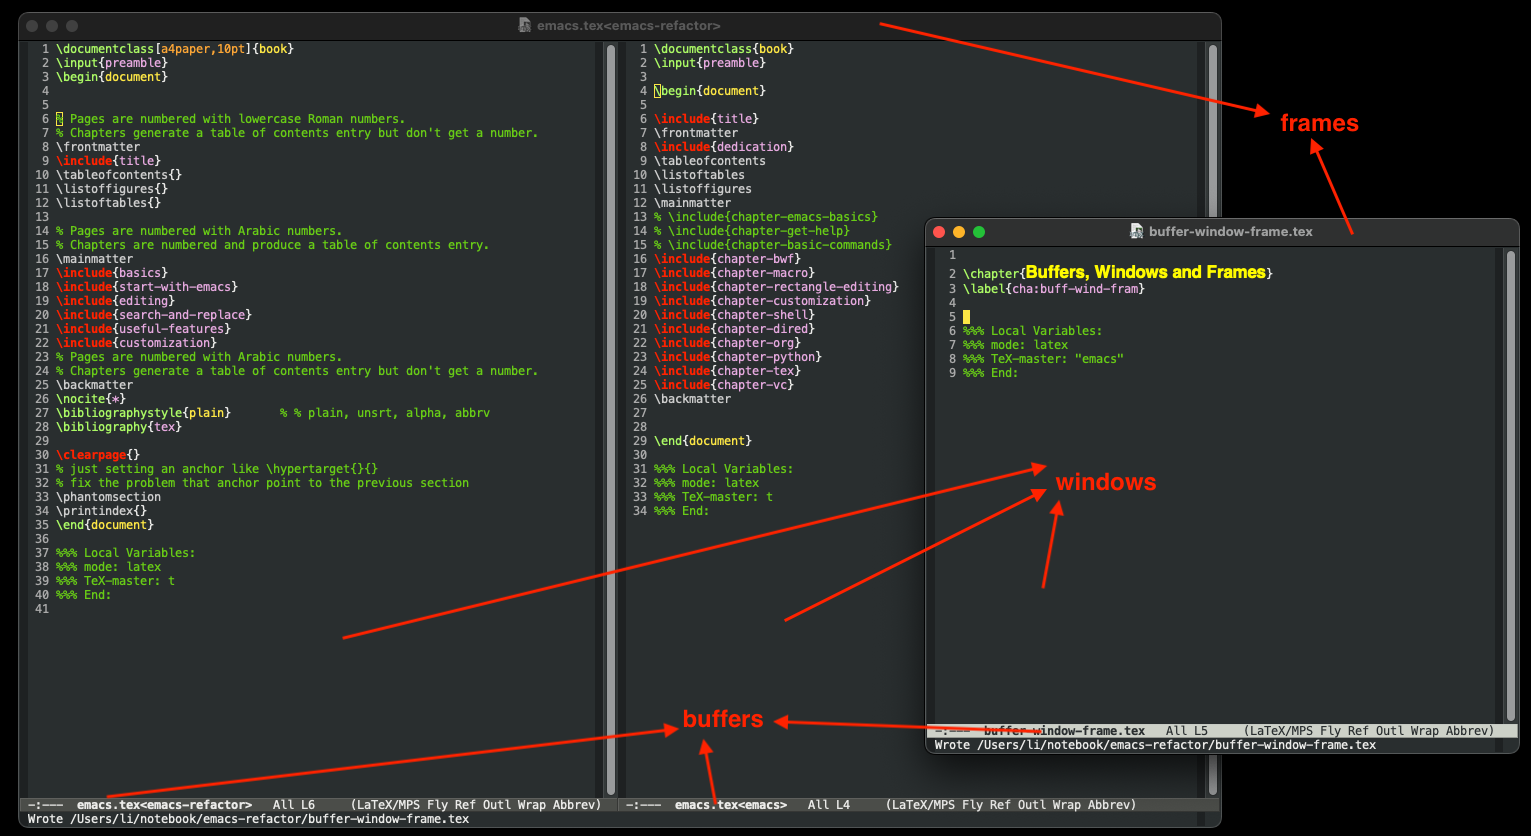
\includegraphics[width=0.9\textwidth]{bwf}  
  \caption{Buffers, windows and frames}
  \label{fig:bwf}
\end{figure}


Buffers are independent of windows and frames.
A Buffer may contains a file or be Emacs-generated.
The name of the buffer that containing a file is the same name with the file.
The name of the buffer that are Emacs-generated has the format \argument{*buffer name*}.
For example, \argument{*Help*, *scratch*, *Messages*} as so on.

\newpage{}
\section{Buffer Commands}
\label{sec:buffer-commands}

\begin{table}[H]
  \centering
  \begin{tabular}{>{\bfseries}ll}
    \toprule
    \head{Binding} & \head{Meaning}\\
    \midrule
    C-x b & move to most recently buffer or the specified buffer\\
    C-x k & delete buffer\\
    C-x C-s & save buffer\\
    C-x s & save all buffers\\
    C-x C-q & toggle read only mode\\
    C-x C-b & list all buffers\\
    \bottomrule
  \end{tabular}
  \caption{Buffer Commands}
  \label{tab:buffer-commands}
\end{table}


\subsection{Buffer List}
\label{sec:buffer-list}

\keyword{C-x C-b} creates a new \argument{*Buffer List*} window on the screen.
It is shown in the following Figure \ref{fig:buffer-list}.
The \argument{CRM} column has the following available values:
\begin{itemize}
\item \keyword{.} : displayed 
\item \keyword{*} : modified
\item \keyword{\%} : read only
\item \keyword{D} : marked for deletion
\item \keyword{>} : marked for display
\item \keyword{S} : marked for saving
\end{itemize}

\begin{figure}[H]
  \centering
  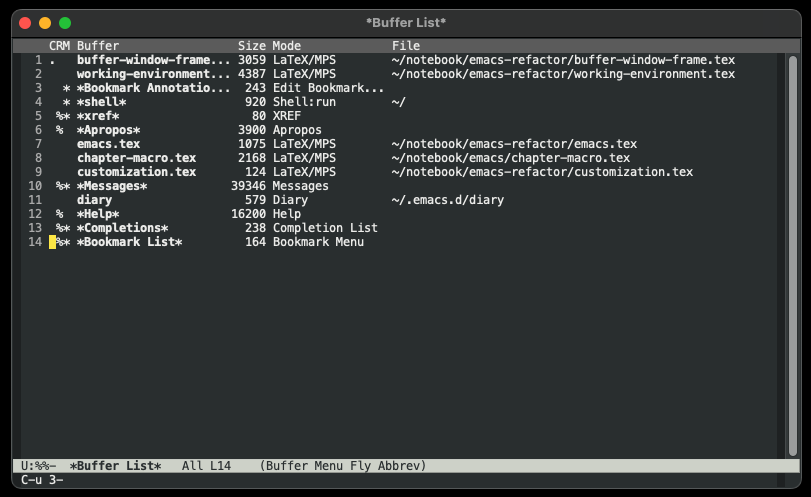
\includegraphics[width=0.9\textwidth]{buffer-list}
  \caption{Buffer list}
  \label{fig:buffer-list}
\end{figure}

\begin{table}[H]
  \centering
  \begin{tabular}{>{\bfseries}ll}
    \toprule
    \head{Keystroke} & \head{Meaning}\\
    \midrule
    C-n or n & down one line\\
    C-p or p & up one line\\
    \midrule
    m & mark buffer to be displayed\\
    d & mark buffer for deletion\\
    s & mark buffer for save\\
    u & unmark buffer\\
    U & remove all marks from all lines\\
    Del & unmark the previous buffer, if there is no mark, move up one line\\
    \midrule
    x & execute other one-letter commands on all marked buffers\\
    v & display buffers marked with \argument{m}\\
    \midrule
    T & toggle whether the menu displays only file buffers\\
    \% & toggle read-only status of buffer\\
    \midrule
    RET & select current line's buffer in place of the buffer menu\\
    V & select current line’s buffer, in View mode\\
    1 & display buffer in a full screen\\
    2 & display this buffer and the next one in horizontal windows\\
    f & replace buffer list with this buffer\\
    o & replace other window with this buffer\\
    C-o & make another window display that buffer\\
    t & visit the tags table in the buffer on this line.\\
    \midrule
    M-s a C-s & incremental search in the marked buffers\\
    M-s a C-M-s & isearch for regexp in the marked buffers\\
    \midrule
    q & quit buffer list\\
    \bottomrule
  \end{tabular}
  \caption{Buffer list commands}
  \label{tab:buffer-list-commands}
\end{table}



\section{Window Commands}
\label{sec:window-commands}

\begin{table}[H]
  \centering
  \begin{tabular}{>{\bfseries}ll}
    \toprule
    \head{Binding} & \head{Meaning}\\
    \midrule
    C-x o & switch to other window\\
    C-x 0 & delete current window\\
    C-x 1 & delete other windows\\
    C-x 2 & split window down\\
    C-x 3 & split window right\\
    \midrule
    C-x \textasciicircum{} & enlarge window vertically\\
    C-x \} & enlarge window horizontally\\
    C-x \{ & shrink window horizontally\\
    \midrule
    C-x - & shrink window if larger than buffer\\
    C-x + & balance window\\
    \bottomrule
  \end{tabular}
  \caption{Window Commands}
  \label{tab:window-commands}
\end{table}

A number of the ``other window'' commands are just the ordinary command with a 4 inserted in it.
For example, to find a file in another window, type \keyword{C-x 4 f}.
To select a different buffer in another window, type \keyword{C-x 4 b}.
These commands save you steps: you do not need move to the other window, give a command and move back.

\subsection{Package "ace-window"}
\label{sec:package-ace-window}

Using \keyword{C-x o} to switch between windows if there are only two windows.
It quickly loses its value when there are more windows.
``ace-window'' is used to solve this problem.
\begin{lstlisting}[language=elisp]
;; Rebind M-o to ace-window
(global-set-key (kbd "M-o") 'ace-window)

;; This is the list of initial characters used in window labels.
;; The characters are used after ace-window command to select the window.
(setq aw-keys '(?a ?s ?d ?f ?g ?h ?j ?k ?l))
\end{lstlisting}

You can swap current window and a specified by calling \keyword{M-o} with a prefix argument \keyword{C-u}.
You can delete the selected window by calling \keyword{ace-window} with a double prefix argument \keyword{C-u C-u}.




\section{Frame Commands}
\label{sec:frame-commands}

\begin{table}[H]
  \centering
  \begin{tabular}{>{\bfseries}ll}
    \toprule
    \head{Binding} & \head{Meaning}\\
    \midrule
    C-x 5 o & switch to other frame\\
    C-x 5 0 & delete current frame\\
    C-x 5 1 & delete other frame\\
    C-x 5 2 & create a new frame on the current buffer\\
    \bottomrule
  \end{tabular}
  \caption{Frame Commands}
  \label{tab:frame-commands}
\end{table}

A number of the ``other frame'' commands are just the ordinary command with a 5 inserted in it.
For example, to find a file in another frame, type \keyword{C-x 5 f}.
To select a different buffer in another frame, type \keyword{C-x 5 b}.
These commands save you steps: you do not need move to the frame, give a command and move back.

%%% Local Variables:
%%% mode: latex
%%% TeX-master: "emacs"
%%% End:


\chapter{Macro}
\label{cha:macro}

In Emacs, a macro is simply a group of recorded keystrokes you can play back over and over again.
Macros are a great way to save yourself \keyword{repetitive} work.


\section{Macro Commands}
\label{sec:macro-commands}

\begin{table}[H]
  \centering
  \begin{tabular}{l>{\bfseries}ll}
    \toprule
    \head{Group} & \head{Binding} & \head{Meaning}\\
    \midrule
    \multirow{2}{*}{define a macro} & C-x ( & start macro definition\\
                 & C-x ) & end macro definition\\
    \midrule
    \multirow{2}{*}{execute macro} & C-x e & call the last defined macro\\
                 & C-x C-k r & apply last macro to all lines in region\\
    \midrule
    edit macro & C-x C-k e & edit macro\\
    \midrule
    \multirow{4}{*}{macro ring} & C-x C-k C-d & delete current macro from macro ring\\
                 & C-x C-k C-t & swap first two elements in macro ring\\
                 & C-x C-k C-p & move to previous macro in macro ring\\
                 & C-x C-k C-n & move to next macro in macro ring\\
    \midrule
    bind macro & C-x C-k b & bind macro\\
    \midrule
    name macro & C-x C-k n & name macro\\
    \bottomrule
  \end{tabular}
  \caption{Macro Commands}
  \label{tab:macro-commands}
\end{table}



\section[Saving Macros]{Naming, Saving, and Executing Your Macros}

\begin{enumerate}
\item Define a macro.
\item name it with \keyword{C-x C-k n}.
\item Open a file.
\item \keyword{M-x insert-kbd-macro RET <macroname> RET}.
\item add \lstinline[language=elisp]|(load-file "<your macro file>")| to \argument{.emacs}.
\item add \lstinline[language=elisp]|(global-set-key "\C-x\C-k<your key>" '<your macro name>)| to \argument{.emacs}.
\end{enumerate}




\section[Macro with Input]{Pausing a Macro for Keyboard Input}
\label{sec:paus-macro-keyb}

When you’re defining a macro, type \keyword{C-u C-x q} at the point where you want the recursive edit to occur.
Emacs enters a recursive edit.
You can tell you’re in a recursive edit because square brackets appear on the mode line.
Nothing you type during the recursive edit becomes a part of the macro.
You can type whatever you want to and then press \keyword{C-M-c} to exit the recursive edit. 



\section{Adding a Query to a Macro}
\label{sec:adding-query-macro}

When you’re defining a macro, type \keyword{C-x q} at the point where you want to add a query.
Nothing happens immediately; go on defining the macro as you normally would.
When you execute the macro and it gets to the point in the macro where you typed \keyword{C-x q}, Emacs prints a query in the minibuffer:
\begin{verbatim}
Proceed with macro? (y, n, RET, C-l, C-r)
\end{verbatim}

Here's the meaning of the options:
\begin{itemize}
\item \keyword{y} means to continue and go on to the next repetition, if any.
\item \keyword{n} means to stop executing the macro but go on to the next repetition, if any.
\item \keyword{Enter} means to stop executing the macro and cancel any repetitions.
\item \keyword{C-r} C-r starts a recursive edit. To exit a recursive edit, press \keyword{C-M-c}.
\item \keyword{C-l} puts the line the cursor in on in the middle of the screen.
\end{itemize}





%%% Local Variables:
%%% mode: latex
%%% TeX-master: "emacs"
%%% End:


\chapter[Working Environment]{Emacs as Working Environment}
\label{cha:emacs-as-working}

\section{Spell Checking}

Emacs provide Ispell interface.
We say ``interfaces'' because Emacs does not include the executable.


On MacOSX, There are two popular software manager \keyword{MacPorts} and \keyword{Homebrew}. You can use any of it to install Ispell.
After installation, use command \lstinline[language=sh]|which ispell| in terminal to locate the Ispell executable file.
In Emacs, type \keyword{C-h a ispell} to get all functions containing the keyword ispell.
You can find the function \argument{ispell-check-version}.
Type \keyword{M-x ispell-check-version} to check whether Ispell is working correctly.
It will show you where should the Ispell executable should be located.
Link the Ispell executable to where Emacs expects Ispell to be:
\begin{lstlisting}[language=sh]
ln -s /opt/local/bin/ispell /usr/local/bin/ispell
\end{lstlisting}



\begin{table}[H]
  \centering
  \begin{tabular}{>{\bfseries}l>{\ttfamily}ll}
    \toprule
    \head{Binding} & \head{Command} & \head{Meaning}\\
    \midrule
                   & ispell-buffer & \\
                   & ispell-region & \\
    M-\$ & ispell-word & \\
    \midrule
                   & ispell-complete-word & \\
    \bottomrule
  \end{tabular}
  \caption{Ispell Commands}
  \label{tab:ispell-commands}
\end{table}

You can use \keyword{C-h f ispell-help} for the options available when a misspelling is encountered.
The options are the following:
\newpage{}

\begin{table}[H]
  \centering
  \begin{tabular}{>{\bfseries}lp{0.6\textwidth{}}}
    \toprule
    \head{Option} & \head{Meaning}\\
    \midrule
    DIGIT & replace the word with a digit offered in the *Choices* buffer\\
    SPC &   accept word this time\\
    i & accept word and insert into private dictionary\\
    a & accept word for this session\\
    A & accept word and place in ‘buffer-local dictionary’\\
    r & replace word with typed-in value.  Rechecked\\
    R & replace word with typed-in value.  Query-replaced in buffer.  Rechecked\\
    x & exit spelling buffer.  Move cursor to original point\\
    X & exit spelling buffer.  Leaves cursor at the current point, and permits the aborted check to be completed later\\
    q & quit spelling session\\
    l & look up typed-in replacement in alternate dictionary\\
    u & like ‘i’, but the word is lower-cased first\\
    m & place typed-in value in personal dictionary, then recheck current word\\
    C-r &recursive edit\\
    \bottomrule
  \end{tabular}
  \caption{Ispell options}
  \label{tab:ispell-options}
\end{table}

\section{Flyspell}
\label{sec:flyspell-1}

Flyspell highlights misspelled words as you type.
There are two mode related with Flyspell: \keyword{flyspell-mode} and \keyword{flyspell-prog-mode}.
The latter mode is designed for programmers.
In this mode Emacs highlights misspellings only in comments or strings.
To check existing text, you run \keyword{M-x flyspell-buffer Enter}.


Flyspell highlights misspelled words in red.
Words that are repeatedly misspelled are highlighted in yellow.


Here are some useful commands in \keyword{flyspell-mode}:
\begin{table}[H]
  \centering
  \begin{tabular}{>{\bfseries}ll}
    \toprule
    \head{Binding} & \head{Meaning}\\
    \midrule
    M-\$ & correct words (using Ispell)\\
    C-M-i & automatically correct word\\
    C-; & automatically correct the last misspelled word\\
    \bottomrule
  \end{tabular}
  \caption{Flyspell commands}
  \label{tab:flyspell-commands}
\end{table}

You can type \keyword{C-M-i} or \keyword{C-;} again to change to another  correct word if the corrected word is not what you want.

\section{Bookmarks}
\label{sec:bookmarks}


It saves any new bookmarks in this file automatically when you exit Emacs.
Bookmark points to a position in a file and not to a piece of text.


\subsection{Bookmark Commands}
\label{sec:bookmark-commands}

\begin{table}[H]
  \centering
  \begin{tabular}{>{\bfseries}ll}
    \toprule
    \head{Binding} & \head{Meaning}\\
    \midrule
    C-x r m & set a bookmark\\
    C-x r b & move to a bookmark\\
    \midrule
    C-x r l & \argument{*Bookmark List*} buffer appears\\
    \bottomrule
  \end{tabular}
  \caption{Bookmark Command}
  \label{tab:bookmark-commands}
\end{table}


\subsection{Bookmark List}
\label{sec:bookmark-list}

\begin{table}[H]
  \centering
  \begin{tabular}{>{\bfseries}ll}
    \toprule
    \head{Binding} & \head{Meaning}\\
    \midrule
    RET, or j & open bookmark\\
    o & open the bookmark in another window and move the cursor to that window\\
    C-o & open the bookmark in another window and keep the cursor in current window\\
    \midrule
    r & rename bookmark\\
    s & save all bookmark\\
    \midrule
    m & mark bookmarks to be displayed in multiple windows\\
    d & mark bookmark for deletion\\
    u & remove mark\\
    \midrule
    x & delete bookmarks marked for deletion\\
    v & display marked bookmarks or the one the cursor is on if none are marked\\
    \midrule
    e & edit (or create) annotation for the current bookmark\\
    a & display annotation for current bookmark\\
    A & display all annotations\\
    \midrule
    q & exit bookmark list\\
    \bottomrule
  \end{tabular}
  \caption{Bookmark list commands}
  \label{tab:bookmark-list-commands}
\end{table}

\section{Shell}
\label{sec:shell}


\subsection{One Command at a Time}
\label{sec:one-command-at}

\begin{table}[H]
  \centering
  \begin{tabular}{>{\bfseries}ll}
    \toprule
    \head{Binding} & \head{Meaning}\\
    \midrule
    M-! & execute command \\
    M-| & execute command with region as input\\
    M-\& & execute command asynchronously in background\\
    \bottomrule
  \end{tabular}
  \caption{One command at a time}
  \label{tab:one-command-at-a-time}
\end{table}

With \keyword{C-u} prefix, the command output is insert to current buffer.

\subsection{Shell Mode}
\label{sec:shell-mode}

To start a shell buffer, type \keyword{M-x shell Enter}.
This creates a buffer named \argument{*shell*}.



How does Emacs know which shell to start?
First, it looks at the variable \argument{shell-file-name}.
Then it looks for a Unix environment variable named \argument{ESHELL}.
Finally it looks for an environment variable named \argument{SHELL}.
If you want to run another particular shell (for example, the zed shell) when you’re in Emacs, you can add the following command to your \argument{.emacs} file:
\begin{lstlisting}
(setq shell-file-name "/bin/zsh")
\end{lstlisting}


When Emacs starts an interactive shell, it runs an additional initialization file after your shell’s normal startup files.
The name of this file is \argument{.emacs\_shell-name}, where \argument{shell-name} is the name of the shell you want to use in Emacs.
It must be located in your home directory.
For example, if you use zsh, you can add Emacs-only startup commands by placing them in the file \argument{.emacs\_zsh}

\begin{table}[H]
  \centering
  \begin{tabular}{l>{\bfseries}ll}
    \toprule
    \head{Group} & \head{Binding} & \head{Meaning}\\
    \midrule
    \multirow{6}{*}{terminal} & C-c C-c & like \keyword{C-c} in terminal\\
                 & C-c C-u & line \keyword{C-u} in terminal\\
                 & M-r & like \keyword{C-r} in terminal\\
                 & M-p & like \keyword{C-p} in terminal\\
                 & M-n & like \keyword{C-n} in terminal\\
                 & C-c SPC & like \keyword{\textbackslash{}} in terminal\\
    \midrule
    \multirow{2}{*}{delete} & C-c C-o & delete output from last command\\
                 & C-c M-o & clear the shell buffer\\
    \midrule
    \multirow{2}{*}{window} & C-c C-r & move first line of output to top of window\\
                 & C-c C-e & move last line of output to bottom of window\\
    \midrule
    \multirow{3}{*}{history} & C-c C-p & move to previous command\\
                 & C-c C-n & move to next command\\
                 & C-c C-l & list the commands you have typed\\
    \midrule
    argument & C-c . & insert previous command argument\\
    \midrule
    \multirow{2}{*}{move} & C-c C-f & \argument{shell-forward-command}\\
                 & C-c C-b & \argument{shell-backward-command}\\
    \midrule
    save & C-c C-s & write the privous output into a file (overwrite)\\
    \bottomrule
  \end{tabular}
  \caption{Shell mode commands}
  \label{tab:shell-mode-commands}
\end{table}


To create multiple shell buffer, you can use \keyword{C-u M-x shell}.


\subsection{Eshell, Shell and Term}
\label{sec:eshell}

Here's the differences:
\begin{itemize}
\item \keyword{M-x shell} starts the standard emacs interface to Operating System's command line interface.

\item \keyword{M-x term} starts the terminal emulator in emacs.
It behaves like a dedicated terminal app, such as xterm, gnome-terminal, puTTY.
It is compatible to more shell apps than emacs shell interface, but standard emacs keys such as moving cursor doesn't work here.

\item \keyword{M-x eshell} starts eshell which is a shell written entirely in emacs lisp.
Note: it is not a bash emulator.
Eshell is a shell by itself, but similar to bash or other shells.

\end{itemize}

Which should you use?
It depends on your preference and needs.
The following is some general guide.

\begin{itemize}
\item shell is the most popular. It is good for general use of classic/standard unix shell commands.
\item term are good if you want to run stuff like \argument{ssh}, or other command line interactive interface (such as \argument{python}), or text based GUI app such as \argument{vim}.
\item Eshell is super fast on startup. If you are a emacs lisp programer, you might prefer eshell because direct access to emacs lisp and better integration with emacs.
\end{itemize}




\section{Directory Editor}
\label{sec:directory-editor}

There are several ways to start directory editing.
If you're not in Emacs, invoke Emacs with a directory name as an argument.
For example, if you want to edit the directory \argument{notebook}, type the following
\begin{lstlisting}[language=sh]
emacs notebook
\end{lstlisting}
If you are in Emacs, you can use \keyword{C-x C-f DIRECTORY} or \keyword{C-x d DIRECTORY} to edit the directory.

\begin{center}
  \begin{longtable}[H]{l>{\bfseries}lp{0.6\textwidth}}
    \toprule
    \head{Group} & \head{Binding} & \head{Meaning}\\
    \midrule
    \endfirsthead

    \toprule
    \head{Group} & \head{Binding} & \head{Meaning}\\
    \midrule
    \endhead

    \midrule
    \multicolumn{3}{c}{{Continued on next page}}\\
    \bottomrule
    \endfoot

    \endlastfoot

    
    \multirow{12}{*}{mark} & m & mark current file\\
                 & * * & mark executable files\\
                 & * @ & mark symlinks\\
                 & * / & mark directories\\
                 & \% m & mark files matching \argument{REGEXP}\\
                 & \% g & mark files containing \argument{REGEXP}\\
                 & \% d & flag for deletion files that match regular expression\\
                 & d & mark file for deletion\\
                 & \# & mark autosave files for deletion\\
                 & \textasciitilde{} & mark backup files for deletion, \keyword{C-u} to prefix remove the flag\\
                 & \& & mark garbage files for deletion\\
                 & u & unmark current file\\
                 & U & unmark all files\\
                 & t & toggle mark\\
                 & * c & change marks on specified files\\
    \midrule
    \multirow{4}{*}{visit} & v & view file read only, \keyword{q} to quit\\
                 & o & find file in another window; move there\\
                 & C-o & find file in another window; don't move there\\
                 & RET & visit file\\
    \midrule
    \multirow{17}{*}{operation} & O & change ownership of file\\
                 & D & delete a file immediately\\
                 & R & rename\\
                 & C & copy marked files\\
                 & G & change group permissions\\
                 & L & load the marked Emacs Lisp files\\
                 & Z & compress or uncompress\\
                 & M & use \keyword{chmod} on current file\\
                 & S & create a symbolic link to this file\\
                 & s & sort the Dired display by date or by filename (toggle)\\
                 & w & copy filename into the kill ring\\
                 & y & display information on the type of the file using the \keyword{file} command\\
                 & ! & run shell command\\
                 & + & create a directory\\
                 & Q & replace matches in all marked files\\
                 & A & do a regular expression search on marked files\\
                 & x & delete the files flagged for deletion\\
    \midrule
                 & n & next line\\
                 & p & previous line\\       
                 & \textasciicircum{} & up directory\\
                 & > & next directory line\\
    \multirow{8}{*}{navigation} & < & previous directory line\\
                 & i & insert this subdirectory into the same dired buffer\\
                 & \$ & hide or show the current directory or subdirectory\\
                 & M-\$ & hide all subdirectories, leaving only their names; repeat command to show\\
                 & C-M-n & move to next subdirectory (if you've inserted subdirectories using \keyword{i})\\
                 & C-M-p & move to previous subdirectory (if you’ve inserted subdirectories using \keyword{i})\\
                 & M-\} & next marked file\\
                 & M-\{ & previous marked file\\
    \bottomrule
    \caption{Dired commands}
    \label{tab:dired-commands}
  \end{longtable}
\end{center}



Here's one trick.
In Dired mode, you can use \keyword{C-x C-q} to change the readonly status.
After is becomes editable, you can edit the dired buffer directly.
When you finish the edit, type \keyword{C-c C-c} to make the change work.

\section{Calendar}
\label{sec:calendar}

To display the calendar, type \keyword{M-x calendar}.
Emacs displays a calendar window with three months: last month, this month, and next month.
Here's my simple configuration in \argument{.emacs} file:
\begin{lstlisting}
;; set the first day of a week to Monday
(setq calendar-week-start-day 1)
;; start calendar at start emacs
(calendar)
\end{lstlisting}

\newpage{}

\begin{table}[H]
  \centering
  \begin{tabular}{l>{\bfseries}ll}
    \toprule
    \head{Group} & \head{Binding} & \head{Meaning}\\
    \midrule
    \multirow{9}{*}{relative move}  & . & today\\
                 & C-f & next day\\
                 & C-b & previous day\\
                 & C-n & forward by week\\
                 & C-p & backward by week\\
                 & M-\} & forward by month\\
                 & M-\{ & backward by month\\
                 & C-x [ & forward by year\\
                 & C-x ] & backward by year\\
    \midrule
    \multirow{7}{*}{absolute move} & C-a & beginning of the week\\
                 & C-e & end of the week\\
                 & M-a & beginning of the month\\
                 & M-e & end of the month\\
                 & M-< & beginning of the year\\
                 & M-> & end of the year\\
                 & g d & go to the specified day\\
    \midrule
    \multirow{4}{*}{scroll} & C-x > & scroll forward by 1 month\\
                 & C-x < & scroll backward by 1 month\\
                 & C-v & scroll forward by 3 months\\
                 & M-v & scroll backward by 3 months\\
    \midrule
    \multirow{4}{*}{holiday}  & a & show holidays for the current calendar window\\
                 & h & show whether today or the specified day is a holiday\\
                 & x & highlight holidays\\
                 & u & remove the highlights\\
    \midrule
    \multirow{7}{*}{add entry} & i d & add day entry\\
                 & i w & add weekly entry\\
                 & i m & add month entry\\
                 & i y & add annual entry\\
                 & i a & add annual entry (the year is included for reference)\\
                 & i c & add cyclic entry\\
                 & i b & add block entry\\
    \midrule
    \multirow{3}{*}{display} & m & highlight entries\\
                 & d & display entry for the current date\\
                 & s & display all entries\\
    \bottomrule
  \end{tabular}
  \caption{Calendar Commands}
  \label{tab:calendar-commands}
\end{table}








%%% Local Variables:
%%% mode: latex
%%% TeX-master: "emacs"
%%% End:


\chapter{Useful Features}
\label{cha:useful-features}

\section{Get Help}
\label{sec:get-help}

Emacs has extensive help.
You should always check the help information to learn how to use the command, how to configure the Emacs, how to search for what you want and so on.


The whole help entry is \keyword{C-h C-h}.
You should read the help buffer carefully to find what the next help information you want to get.


For example, if you want to replace some string but forget the key binding and the function, you can use \keyword{C-h a replace Enter}. You will get all the functions containing the keyword \keyword{replace}.


\section{Auto Fill}
\label{sec:auto-fill}

\subsection{Dynamic Expanding}
\label{sec:dynamic-expanding}


\keyword{M-/} runs the command \argument{dabbrev-expand}.
It expands previous word ``dynamically''.
Expands to the most recent, preceding word for which this is a prefix.
If no suitable preceding word is found, words following point are considered.
It also search other buffers.

\subsection{Auto Correct Word}
\label{sec:auto-correct-word}

If flyspell-mode is enabled,
\keyword{C-M-i} runs the command \argument{flyspell-auto-correct-word}.
This command proposes various successive corrections for the current word.
If invoked repeatedly on the same position, it cycles through the possible corrections of the current word.

Otherwise, \keyword{C-M-i} runs corresponding command to do completion.

\subsection{Auto Fill Commands}
\label{sec:auto-fill-commands}
If you are in minibuffer, you can use \keyword{Tab} to auto-fill commands and filenames.

For example, type \keyword{M-x open Tab}. If there are only one command matching the ``open'' prefix, it will be auto-filled.
If there are more commands matching the prefix, type \keyword{Tab} again to get all candidates. In AUCTeX mode, you use \keyword{C-c C-m} to start a macro.
In the minibuffer, you can use \keyword{Tab} to auto-fill \LaTeX{}\xspace command.

If you type \keyword{C-x C-f} to open a file. In the minibuffer, you can use \keyword{Tab} to auto-fill the filename or use \keyword{Tab Tab} to get all candidates.



\section{Canceling Commands}
\label{sec:canceling-commands}

When you want to cancel any command that’s in progress, press \keyword{C-g}.
The word \keyword{Quit} appears in the command area.
This command is helpful when you are stuck in the minibuffer and didn’t really mean to go there.
Depending on what you were doing, you may have to press \keyword{C-g} a few times.


\section{Undoing Changes}
\label{sec:undoing-changes}

What happens if you make a mistake while you’re editing? You can undo your changes by \keyword{undo} function.
Type \keyword{C-h k undo Enter} and choose your favorite key binding.


What if you’d like to redo a command after you type undo?
There is no formal redo command, but you can use undo in the following way.
Just move the cursor in any direction, and use undo again.
Emacs redoes the last command you undid.
You can repeat it to redo previous undos.


\section{History Commands}
\label{sec:history-commands}

Emacs will record the commands you have used before, so you can reuse them to avoiding typing them again to save you time.


\keyword{C-x Esc Esc} will let you edit then re-evaluate the last complex command.
A \keyword{ command} is one that used the minibuffer.
The command is placed in the minibuffer as a Lisp form for editing.
The result is executed, repeating the command as changed.
In the minibuffer, you can use \keyword{M-n} and \keyword{M-p} to navigate fore ward and backward the history.


\keyword{C-x z} repeats the most recently executed command.


In LaTeX mode, when you use \keyword{C-c C-e} to insert an environment, 
In the minibuffer, you can use \keyword{M-n} and \keyword{M-p} to navigate fore ward and backward the history.


\section{C-u}
\label{sec:c-u}

\keyword{C-u} runs the command \argument{universal-argument}.
It has the following situations:
\begin{itemize}
\item following \keyword{digits}, it will repeat the following command \keyword{digits} times
\item following \keyword{- or - digits}, some commands support negative digits and it will repeat the following command \keyword{1 or digits} times in the opposite direction
\item without digits or minus sign, it provides 4 as argument
\item repeating \keyword{C-u} without digits or minus sign many times, it multiplies the argument by 4 each time
\item for some commands, just \keyword{C-u} by itself serves as a flag that change the command function.
\end{itemize}



\section{Saving Positions in Registers}
\label{sec:saving-posit-regist}

Typing \keyword{C-x r SPC (point-to-register)}, followed by a character \keyword{r}, saves both the position of point and the current buffer in register \keyword{r}.
The register retains this information until you store something else in it.

The command \keyword{C-x r j r} switches to the buffer recorded in register \keyword{r}, pushes a mark, and moves point to the recorded position.
(The mark is not pushed if point was already at the recorded position, or in successive calls to the command.)
The contents of the register are not changed, so you can jump to the saved position any number of times.


\section{rgrep}
\label{sec:rgrep}

\keyword{M-x rgrep} can recursively search the content in the directory and files you specified.
%%% Local Variables:
%%% mode: latex
%%% TeX-master: "emacs"
%%% End:


\chapter{Customization}

\section{Mute beep sound}

\lstset{language=Sh}
\begin{lstlisting}
  echo 'set bell-style none' >> ~/.inputrc
\end{lstlisting}



\documentclass[a4paper,10pt]{book}
\usepackage[english]{babel}     
\usepackage[utf8]{inputenc}     % accent symbols
\usepackage[T1]{fontenc}
\usepackage{lmodern}
\usepackage{microtype}
\usepackage{natbib}
\usepackage{tocbibind}          
\usepackage{amsmath}            % math symbols
\usepackage{amsthm}             % math symbols
\usepackage[colorlinks=true,linkcolor=red]{hyperref} % hyper link

% for code
\usepackage{listings}
\usepackage{color,xcolor}
\definecolor{mygreen}{rgb}{0,0.6,0}
\definecolor{mygray}{rgb}{0.9,0.9,0.9}
\definecolor{mymauve}{rgb}{0.58,0,0.82}
\lstset{
backgroundcolor=\color{mygray},
numbers=left,                    
columns=fullflexible,
breaklines=true,      
captionpos=b,         
tabsize=4,            
commentstyle=\color{mygreen}, 
escapeinside={\%*}{*)},       
keywordstyle=\color{blue},    
% stringstyle=\color{mymauve}\monaco,
frame=single,                        
rulesepcolor=\color{red!20!green!20!blue!20},
% identifierstyle=\color{red},
%% language=c++,
basicstyle=\tiny
}

\usepackage{indentfirst}
\setlength{\parindent}{2em}
\usepackage[onehalfspacing]{setspace}
% graph
\usepackage{pdfpages}
\usepackage{graphicx}
% box
\usepackage{booktabs}
\usepackage{tcolorbox}

%% user defined command
\newcommand{\keyword}[1]{\textbf{#1}}
\newcommand{\keywords}[1]{\textbf{#1}}
\newcommand{\lcmd}[1]{\texttt{#1}}
\newcommand{\head}[1]{\textnormal{\textbf{#1}}}
\newcommand{\itwords}[1]{\textit{#1}}

\usepackage{float}
% all symbols
\usepackage{tipa}
\usepackage{tipx}

\usepackage{datetime}
% \usepackage{movie15}


% variable
% TODO
\newcommand{\pdfauthor}{李明明}
\newcommand{\pdftitle}{工作}
\newcommand{\pdfsubject}{工作中的经验与教训}
\newcommand{\pdfkeywords}{工作经验与教训}
\newcommand{\bookname}{工作收获}
\newcommand{\bookoneword}{工作中吸取的经验和教训}
\newcommand{\timeandcompany}{2020年12月1日}

\usepackage{bm}
\usepackage{amsfonts}
\begin{document}

\newcommand{\mytitle}{Git}
\newcommand{\firstcreated}{Mar 16, 2023}

\begin{titlepage}

\newcommand{\HRule}{\rule{\linewidth}{0.5mm}} % Defines a new command for the horizontal lines, change thickness here

\center                         % Center everything on the page
 
%----------------------------------------------------------------------------------------
%	HEADING SECTIONS
%----------------------------------------------------------------------------------------


\includegraphics[width=0.5\textwidth]{logo}\\[1cm] % Include a department/university logo - this will require the graphicx package

%----------------------------------------------------------------------------------------
%	TITLE SECTION
%----------------------------------------------------------------------------------------

\HRule\\[0.4cm]
{ \huge \bfseries \mytitle}\\[0.4cm] % Title of your document
\HRule\\[1.5cm]
 
%----------------------------------------------------------------------------------------
%	AUTHOR SECTION
%----------------------------------------------------------------------------------------

\begin{minipage}{0.4\textwidth}
\begin{center} \large
Mingming \textsc{Li}\\ % Your name
\end{center}

\end{minipage}\\[2cm]


%----------------------------------------------------------------------------------------
%	DATE SECTION
% ----------------------------------------------------------------------------------------
\vfill
{\large First Created: \firstcreated}\\
{\large Last Modified: \today}\\[2cm] % Date, change the \today to a set date if you want to be precise



\end{titlepage}


%%% Local Variables:
%%% mode: latex
%%% Tex-master: "git"
%%% End:

% Pages are numbered with lowercase Roman numbers.
% Chapters generate a table of contents entry but don't get a number.
\frontmatter

\tableofcontents{}
\listoffigures{}
\listoftables{}

% Pages are numbered with Arabic numbers.
% Chapters are numbered and produce a table of contents entry.
\mainmatter 


\chapter{\LaTeX\xspace Base}


\section{What is \LaTeX}
\label{sec:what-latex}

\LaTeX\index{latex} is a document markup language\footnote{Just like HTML}. It separate format from content.

\section{Reason to Use It}


Because \LaTeX \xspace{} is a markup language, you should learn it before you can use it.
So why should you spend so much time to learn it while there is so much document creator like Word, Pages?

There is several reasons that push me to select it.
\begin{itemize}
\item It provides powerful edit ability. You can almost get whatever you want to show, especially the mathematical equations.
\item Because it separate the format and the content, it is easy to do format alteration in the full document domain.
\item Once you create your own template, it is easy to wreate document with the template applied, saving so much time in format. 
\end{itemize}



\section{Logical formatting}
\index{latex!{logical formatting}}
\lstset{language=TeX}
\begin{lstlisting}
  \documentclass{article}
  \begin{document}
  \title{Example}
  \author{Mingming Li}
  \date{2022/11/04}
  \maketitle{}
  \section{Logical Formatting}
  This example show logical formatting.
  \end{document}
\end{lstlisting}

We do not specify the font family, font size, and so on, instead we tell \LaTeX \ the \keyword{class}, the \keyword{author}, or the \keyword{section} and let \LaTeX{} to format it.



\section{Command}
\index{latex!command}
LaTeX commands begin with a backslash, followed by big or small letters.
LaTeX commands are usually named with small letters and in a descriptive way.
There are exceptions: a backslash and just one special character.
Commands may have arguments, given in curly braces or in square brackets.

Calling a command looks like the following:


\begin{lstlisting}
  \command
  \command{argument}
  \command[optional argument]{argument}
\end{lstlisting}

For example

\begin{lstlisting}
  {\large Title}
  \include{preamble}
  \documentclass[12pt]{article}
\end{lstlisting}

\section{Comment}
\index{latex!comment}
The percent sing(\%) introduces a \keyword{comment}.


\begin{lstlisting}
  \include{preamble}  % include preamble tex file
\end{lstlisting}

\section{Environment}
\label{sec:environment}
\index{latex!environment}
\begin{lstlisting}
  % This is the environment syntax.
  \begin{name}[optional argument]{argument}
    ...
  \end{name}
\end{lstlisting}


\section{Breaks and Empty Lines}
\label{sec:breaks-empty-lines}

LaTeX treats multiple spaces just like a single space.
Also, a single line break has the same effect like a single space.
It doesn't matter how you arrange your text in the editor using spaces or breaks, the output will stay the same.
A blank line denotes a paragraph break.
Like spaces, multiple empty lines are treated as one.
Briefly said, spaces separate words, empty lines separate paragraphs.


\section{Special Symbols}
\label{sec:special-symbols}
\index{latex!symbols}
By putting a backslash before such a special symbol, we turned it into a LaTeX command.
This command has the only purpose of printing out that symbol.



\begin{lstlisting}
  \%  % just print % symbol
  \textbackslash % just print \ symbol
\end{lstlisting}




\section{Create Your Own Commands}

\begin{lstlisting}
  % This is the full definition of creating you own command.
  \newcommand{command}[arguments][optional]{definition}
\end{lstlisting}


\begin{lstlisting}
  % With no arguments.
  \newcommand{\TUG}{TeX Users Group\xspace}
  \TUG

  % With arguments.
  \newcommand{\keyword}[1]{\textbf{#1}}
  \keyword{declrations}

  % With optional arguments.
  \newcommand{\keyword2}[2][\bfseries]{{#1#2}}
  \keyword2[\itshape]{declarations}
\end{lstlisting}


\section{Get Help}
Three ways to get help about the package:
\begin{enumerate}
  
\item 
\begin{lstlisting}[language=sh]
    texdoc <package>
\end{lstlisting}

\item
\begin{lstlisting}[language=sh]
    kpsewhich <package>.sty
\end{lstlisting}

\item Visit the website: \url{http://ctan.org/pkg}

\end{enumerate}

\section{Install Extra Packages}
\label{sec:inst-extra-pack}

The easy way is to use the terminal to install extra packages:

\begin{lstlisting}[language=sh]
# Tex Live manager
tlmgr install <package>
\end{lstlisting}




\section{Floats}
\index{latex!float}


\LaTeX\xspace provides two floating environments, namely,
\argument{figure} and \argument{table}. They are briefly called
\keyword{floats}. Their content may float to a place where it's the
optimum for the page layout.


Here's the float placement options:
\begin{itemize}
\item h: here. The float may appear where it's been written in the source code.
\item t: top. Placing at the top of a page is permitted.
\item b: bottom. The float may appear at the bottom of a page.
\item p: page. The float is allowed to appear on a separate page,
  where only floats may reside but no normal text.
\item !: tells LaTeX to try harder! Some constraints may be ignored,
  easing the placement.
\end{itemize}


The most flexible is using the placement \argument{[!htbp]}, allowing a float
everywhere.







\section{Modes}
\label{sec:modes}

LaTeX knows three general \keyword{modes}:
\begin{itemize}
\item The \keyword{paragraph mode}: The text is typeset as a sequence of words in lines, paragraphs, and pages.
\item The \keyword{left-to-right mode}: The text is also considered to be a sequence of words, but LaTeX typesets it from left to right without breaking the line. 
\item The \keyword{math mode}: Letters are treated as math symbols. A lot of symbols can be used, most of them exclusively in this mode. Such symbols are roots, sum signs, relation signs, math accents, arrows, and various delimiters like brackets and braces. Space characters between letters and symbols are ignored. 
\end{itemize}



%%% Local Variables:
%%% mode: latex
%%% TeX-master: "latex"
%%% End:

\documentclass[a4paper,10pt]{book}
\input{preamble}
\begin{document}


% Pages are numbered with lowercase Roman numbers.
% Chapters generate a table of contents entry but don't get a number.
\frontmatter{}
\include{title}
\cleardoublepage{}
\phantomsection{}
\tableofcontents{}
\cleardoublepage{}
\phantomsection{}
\listoffigures{}
\cleardoublepage{}
\phantomsection{}
\listoftables{}


% Pages are numbered with Arabic numbers.
% Chapters are numbered and produce a table of contents entry.
\mainmatter{}
\include{basics}
\include{start-with-emacs}
\include{editing}
\include{search-and-replace}
\include{buffer-window-frame}
\include{macro}
\include{working-environment}
\include{useful-features}
\include{customization}
\include{latex}
\include{version-control}
\include{org}

\include{python}
% Pages are numbered with Arabic numbers.
% Chapters generate a table of contents entry but don't get a number.
\backmatter{}
\cleardoublepage{}
\phantomsection{}
\nocite{*}
\bibliographystyle{plain}       % % plain, unsrt, alpha, abbrv
\bibliography{tex}

\cleardoublepage{}
% just setting an anchor like \hypertarget{}{}
% fix the problem that anchor point to the previous section
\phantomsection{}                 
\printindex{}
\end{document}

%%% Local Variables:
%%% mode: latex
%%% TeX-master: t
%%% End:




\chapter[Commands and Environments]{Common Commands and Environments}

\section{Commands}
\label{sec:commands}


\lstset{language=TeX}
\begin{lstlisting}
% produces some space.
\quad                           

% ended a line.
\\ or \newline                  

% prevents a line break at the current position.
\nolinebreak                    

%  `` and '' is the quotation in latex. 
``hello''                       

% ragged left  
{\raggedleft Example text}      
% ragged right
{\raggedright Example text}     
% centering 
{\centering Example text}        


% tells LaTeX to produce a file with the extension .toc. 
% This file will be used to generate a table of contents. 
% We had to typeset twice: in the first run, the .toc file
% was written and in the second run, LaTeX read it and processed it.
\tableofcontents{}              


% causes a page break. Furthermore, the text has been 
% stretched to fill the page down to the bottom.
\pagebreak{}
% breaks the page as well, but it doesn't stretch the
% text: the remaining space of the page will stay empty.
\newpage{}
% forbids page breaking
\nopagebreak{}


% to squeeze more text onto a page. 
\enlargethispage{2\baselineskip}



% placed a superscripted number at the current position.
% Further, it prints its argument text into the bottom of 
% the page, marked by the same number
\footnote{text}
% modify the line that separates footnotes from the text 
% is produced by the command \footnoterule.
\renewcommand{\footnoterule}{\noindent\smash{\rule[3pt]{\textwidth}{0.4pt}}}

\rule[raising]{width}{height}
% draw a line 1pt at thick, as wide as text, raised a bit by 3 pt
\rule[3pt]{\textwidth}{1pt}

% \smash, we let our line pretend to have a height and a depth of 
zero, so it's occupying no vertical space at all


% when we use \footnote inside an argument, there will be an error. 
% \protect simply prevents this processing error. 
\protect{}
\section{Section \protect{\footnote{text}}}
% to avoid footnote appearing in heading and table of content
\section[title without footnote]{Section \protect{\footnote{text}}}



% ends the current page and causes all already defined figures and
tables to be printed out.
\clearpage{}

\cleardoublepage{}


% To be able to refer to a certain point, we have to mark it by a label.
% We can reference to the name of that label afterwards.
% notice , typeset twice to produce the cross reference
\label % marks the position
\ref % prints the number of the element we refer to 
\pageref % prints the page number of that element


\end{lstlisting}


\section{Environments}
\label{sec:environments}


\begin{lstlisting}
% quote long text
\begin{quotation}
\end{quotation}
\end{lstlisting}

\begin{lstlisting}
% center environment
\begin{center}
\end{center}
\end{lstlisting}


%%% Local Variables:
%%% mode: latex
%%% TeX-master: "latex"
%%% End:

\chapter{Font}

\section{Shape}
\begin{table}[!h]
  \centering
  \caption{Font Command}
  
  \begin{tabular}{ccc}
    \toprule
    \head{Command} & \head{Explaination} & \head{Output} \\
    \midrule
    \verb|\textbf{Example}| & bold font & \textbf{Example} \\
    \verb|\textit{Example}| & italic & \textit{Example} \\
    \verb|\textsl{Example}| & slated & \textsl{Example} \\
    \verb|\textsc{Example}| & small caps & \textsc{Example} \\
    \verb|\textup{Example}| & & \textup{Example} \\
    \verb|\textmd{Example}| & medium & \textmd{Example} \\
    \verb|\textnormal{Example}| & & \textnormal{Example} \\
    \verb|\textsf{Example}| & sans-serif & \textsf{Example} \\
    \verb|\texttt{Example}| & typewritter & \texttt{Example} \\
    \verb|\textrm{Example}| & Roman & \textrm{Example} \\
    \bottomrule
    
  \end{tabular}
  
\end{table}


\begin{table}[!h]
  \centering
  \caption{Font Declaration}
  \begin{tabular}{ccc}
    \toprule
    \head{Declaration} & \head{Explaination} & \head{Output} \\
    \midrule
    \verb|{\itshape Example}| & italic & {\itshape Example} \\
    \verb|{\bfseries Example}| & bold font & {\bfseries Example} \\
    \verb|{\slshape Example}| & slated & {\slshape Example} \\
    \verb|{\scshape Example}| & small caps & {\scshape Example} \\
    \verb|{\upshape Example}| & & {\upshape Example} \\
    \verb|{\mdseries Example}| & medium & {\mdseries Example} \\
    \verb|{\normalfont Example}| & & {\normalfont Example} \\
    \verb|{\sffamily Example}| & sans-serif & {\sffamily Example} \\
    \verb|{\ttfamily Example}| & typewritter & {\ttfamily Example} \\
    \verb|{\rmfamily Example}| & roman & {\rmfamily Example} \\
    \bottomrule
    
  \end{tabular}
  
\end{table}


\begin{table}[!hbp]
  \centering
  \caption{Font Emphasized}
  \begin{tabular}{ccc}
    \toprule
    \head{Command} & \head{Explaination} & \head{Output} \\
    \midrule
    \verb|\emph{Example}| & emphasized & \emph{Example} \\
    \bottomrule
  \end{tabular}
\end{table}
\clearpage



\section{Size}
\begin{table}[!hbp]
  \centering
  \caption{Font Size}
  \begin{tabular}{cc}
    \toprule
    \head{Command} & \head{Output} \\
    \midrule
    \verb|\tiny{Example}| & \tiny{Example} \\
    \verb|\scriptsize{Example}| & \scriptsize{Example} \\
    \verb|\footnotesize{Example}| & \footnotesize{Example} \\
    \verb|\small{Example}| & \small{Example} \\
    \verb|\normalsize{Example}| & \normalsize{Example} \\
    \verb|\large{Example}| & \large{Example} \\
    \verb|\Large{Example}| & \Large{Example} \\
    \verb|\LARGE{Example}| & \LARGE{Example} \\
    \verb|\huge{Example}| & \huge{Example} \\
    \verb|\Huge{Example}| & \Huge{Example} \\
    \bottomrule
  \end{tabular}
\end{table}



\chapter{Box}

\section{parbox}

We used the command \lstinline{\parbox} to create a column.

\begin{lstlisting}
  \parbox[alignment]{width}{text}
  \parbox[alignment][height][inner alignment]{width}{text}
\end{lstlisting}

\begin{description}
\item[alignment] Optional argument for the vertical alignment. State t to align at the top line of the box; write b to align at its bottom line. The default behavior is to place the box such that its center is in line with the center of the current text line.
\item[height] If this optional argument isn't given, the box will have just the natural height of the text inside. Use this argument if you want to change the height of the box to make it bigger or smaller.
\item[inner alignment] Especially, if the height of the box is different to the natural height of the contained text, you might want to adjust the text position. The argument means:
  \begin{itemize}
  \item c: vertically center the text in the box
  \item t: place text at the top of the box
  \item b: place text at its bottom
  \item s: stretch the text vertically if possible
  \end{itemize}
  
\end{description}

\begin{lstlisting}
Text line
\quad\fbox{\parbox[b]{1.8cm}{this parbox is aligned at its bottom line}}
\quad\fbox{\parbox{1.5cm}{center-aligned parbox}}
\quad\fbox{\parbox[t]{2cm}{another parbox aligned at its top line}}
\end{lstlisting}


Text line
\quad\fbox{\parbox[b]{1.8cm}{this parbox is aligned at its bottom line}}
\quad\fbox{\parbox{1.5cm}{center-aligned parbox}}
\quad\fbox{\parbox[t]{2cm}{another parbox aligned at its top line}}


\section{fbox}

This command show the frame out.

\begin{lstlisting}
  \fbox{Example}
\end{lstlisting}

\fbox{Example}


\section{minipage}
\label{sec:minipage}

Parboxes are suitable for boxes with only a little text inside.
In case of a box containing a large amount of text, the closing brace could easily be forgotten or overlooked.
The minipage environment would then be a better choice.


\begin{lstlisting}
  \begin{minipage}{3cm}
    Hello World!
  \end{minipage}
\end{lstlisting}

\begin{minipage}{3cm}
  Hello World!
\end{minipage}

\section{mbox}
\label{sec:mbox}


\begin{lstlisting}
  \mbox{Hello World}
\end{lstlisting}

\mbox{Hello World}

\section{tcolorbox}
\label{sec:tcolorbox}

\begin{lstlisting}
\begin{tcolorbox}
  \mbox{Hello World}
\end{tcolorbox}
\end{lstlisting}

\begin{tcolorbox}
  \mbox{Hello World}
\end{tcolorbox}


\chapter{Lists}
\label{cha:lists}


\section{Bulleted Lists}

\begin{lstlisting}
  \begin{itemize}
  \item geometry
  \item amsmath
  \end{itemize}
\end{lstlisting}


\begin{itemize}
\item geometry
\item amsmath
\end{itemize}


\section{Numbered Lists}
\begin{lstlisting}
  \begin{enumerate}
  \item geometry
  \item amsmath
  \end{enumerate}
\end{lstlisting}


\begin{enumerate}
\item geometry
\item amsmath
\end{enumerate}




\section{Definition Lists}
\begin{lstlisting}
  \begin{description}
  \item[paralist] provides compact lists and list versions that
    can be used within paragraphs, helps to customize labels and
    layout
  \item[enumitem] gives control over labels and lengths
    in all kind of lists
  \item[mdwlist] is useful to customize description lists, it
    even allows multi-line labels. It features compact lists and
    the capability to suspend and resume.
  \item[desclist] offers more flexibility in definition list
  \item[multenum] produces vertical enumeration in multiple
    columns
  \end{description}
\end{lstlisting}


\begin{description}
\item[paralist] provides compact lists and list versions that
  can be used within paragraphs, helps to customize labels and
  layout
\item[enumitem] gives control over labels and lengths
  in all kind of lists
\item[mdwlist] is useful to customize description lists, it
  even allows multi-line labels. It features compact lists and
  the capability to suspend and resume.
\item[desclist] offers more flexibility in definition list
\item[multenum] produces vertical enumeration in multiple
  columns
\end{description}


%%% Local Variables:
%%% mode: latex
%%% TeX-master: "latex"
%%% End:

\chapter{Tables}

\section[Table]{tabular}
\label{sec:tabular}


LaTeX provides the \argument{tabular} environment for typesetting simple and complex tables which can be nested.


\begin{lstlisting}
  \newcommand{\head}[1]{\textnormal{\textbf{#1}}}
  \begin{tabular}{ccc}
    \hline                      % Draw a horizontal line over whole width of the table
    \head{Command} & \head{Declaration} & \head{Output} \\
    \hline
    \verb|\textrm| & \verb|\rmfamily| & \rmfamily Example text \\
    \verb|\textsf| & \verb|\sffamily| & \sffamily Example text \\
    \verb|\texttt| & \verb|\ttfamily| & \ttfamily Example text \\
    \hline
  \end{tabular}
\end{lstlisting}


\begin{tabular}{ccc}
  \hline
  \head{Command} & \head{Declaration} & \head{Output} \\
  \hline
  \verb|\textrm| & \verb|\rmfamily| & \rmfamily Example text \\
  \verb|\textsf| & \verb|\sffamily| & \sffamily Example text \\
  \verb|\texttt| & \verb|\ttfamily| & \ttfamily Example text \\
  \hline
\end{tabular}

Within tabular, three types of lines may be used:
\begin{itemize}
\item \lstinline|\hline|: draws a horizontal line over the whole width of the table
\item \lstinline|\cline{m-n}|: draws a horizontal line starting at the beginning of column \argument{m} and ending at the end of column \argument{n}
\item \lstinline|vline|: draws a vertical line over the full height and depth of the current row
\end{itemize}


The options understood by the \argument{tabular} environment are as follows:
\begin{itemize}
\item \argument{l}: for left alignment.
\item \argument{c}: for centered alignment.
\item \argument{r}: for right alignment.
\item \lstinline|p{width}|: for a "paragraph" cell of a certain width. . If you place several \argument{p} cells next to each other, they will be aligned at their top line. It's equivalent to using \lstinline|\parbox[t]{width}| within a cell.
\item \lstinline|@{code}| inserts \argument{code} instead of empty space before or after a column. This might also be some text or it could be left empty to avoid this space.
\item \argument{|}: stands for a vertical line.
\item \lstinline|*{n}{options}| is equivalent to \argument{n} copies of options, where n is a positive integer and options may consist of one or more column specifiers including * as well.
\end{itemize}





\section[Multiple Columns]{Spanning Entries Over Multiple Columns}
\label{sec:spann-entr-over}


\begin{lstlisting}
\begin{tabular}{@{}l*2{>{\textbackslash\ttfamily}l}l<{Example text}@{}}
  \toprule
  & \multicolumn{2}{c}{\head{Input}} & \multicolumn{1}{c}{\head{Output}}\\
  & \normal{\head{Command}} & \normal{\head{Declaration}} & \normal{}\\
  \cmidrule(lr){2-3}\cmidrule(l){4-4}
  Family & textrm&rmfamily & \rmfamily\\
  & textsf & sffamily & \sffamily\\
  & texttt & ttfamily & \ttfamily\\
  \bottomrule
\end{tabular}
  
\end{lstlisting}

\begin{tabular}{@{}l*2{>{\textbackslash\ttfamily}l}l<{Example text}@{}}
  \toprule
  & \multicolumn{2}{c}{\head{Input}} & \multicolumn{1}{c}{\head{Output}}\\
  & \normal{\head{Command}} & \normal{\head{Declaration}} & \normal{}\\
  \cmidrule(lr){2-3}\cmidrule(l){4-4}
  Family & textrm&rmfamily & \rmfamily\\
  & textsf & sffamily & \sffamily\\
  & texttt & ttfamily & \ttfamily\\
  \bottomrule
\end{tabular}


\section{Adding Captions to Tables}
\label{sec:adding-capt-tabl}


\begin{lstlisting}
\begin{table}
  \centering
  \begin{tabular}{}
    
  \end{tabular}
  \caption{Caption}
  \label{tab:caption}
\end{table}  
\end{lstlisting}


\chapter{Figure}

\argument{graphicx} is need to insert figure into you document.


LaTeX supports the following file types:
\begin{itemize}
\item \argument{PNG, JPG}, and \argument{PDF} if you directly compile
  to PDF (\keyword{pdfLaTeX})
\item \argument{EPS} if you compile to DVI and convert to PS and PDF (traditional LaTeX)
\end{itemize}


\begin{tcolorbox}
  \begin{itemize}
  \item PS: PostScript
  \item EPS: Encapsulated PostScript
  \item DVI: Device Independent Format
  \end{itemize}
\end{tcolorbox}


You don't need to specify a filename extension, it will be
automatically added.
Don't use blanks in the filename or path!
Blanks and special characters may cause problems with \lstinline|\includegraphics|.
If such symbols in filenames are required, load the package
\argument{grffile} to try to fix it.


\begin{lstlisting}
  \usepackage[demo]{graphicx}
  \begin{figure}
    \centering
    \includegraphics{test}
    \caption{Test figure}
  \end{figure}
\end{lstlisting}

Because we specified the \argument{demo} option, \argument{graphicx}
doesn't require a file \argument{test.png} or any other file; instead
it's just printing a black filled rectangle. This is useful for
testing or if you would like to discuss a LaTeX problem in an online
forum, but don't wish to publish your pictures.


\begin{lstlisting}
  % syntax
  \includegraphics[k=v]{file name}
\end{lstlisting}

Here are the most popular ones:
\begin{itemize}
\item \argument{width}: \lstinline|width=0.8\textwidth|
\item \argument{height}
\item \argument{scale}: \lstinline|scale=0.5|
\item \argument{angle}: \lstinline{angle=90}
\end{itemize}







\chapter{Listing Content and References}
\label{cha:list-cont-refer}



\section{Table of Content}
\label{sec:table-content}

\begin{table}[H]
  \centering
  \begin{tabular}{>{\textbackslash\ttfamily}ll}
    \toprule
    \normal{\head{Command}} & \head{Level}\\
    \midrule
    part & -1 (\argument{book} and \argument{report} class)\\
    chapter & 0 (not available in \argument{article})\\
    section & 1\\
    subsection & 2\\
    subsubsection & 3\\
    paragraph & 4\\
    subparagraph & 5\\
    \bottomrule
  \end{tabular}
  \caption{Depth of the TOC}
  \label{tab:depth-of-toc}
\end{table}


There's a variable representing the level, namely, \lstinline|\tocdepth|.
It's an integer variable which we call a \keyword{counter}.

There are two basic ways to adjust a counter value:
\begin{lstlisting}
% specifies an integer value of 'n' for the counter 'name'.
\setcounter{name}{n}            
% adds the integer value of 'n' to value of the counter 'name'. 'n' may be negative.
\addtocounter{name}{n}          


\setcounter{tocdepth}{3}
% you can raise or lower the level without knowing its number.
\addtocounter{tocdepth}{1}
\end{lstlisting}


\subsection{Adding entries manually}
\label{sec:adding-entr-manu}

\begin{lstlisting}
% file extension:
% toc: table of contents file
% lof: list of figures file
% lot: list of tables file

% sectional unit: part, chapter, section, subsection, paragraph, subparagraph
\addcontentsline{file extension}{sectional unit}{text}

% In contrary to \addcontentsline, the argument entry is written directly to the file
% without any additional formatting. You may choose any formatting you like.
\addtocontents{file extension}{entry}


% Examples
\addcontentsline{toc}{chapter}{Preface}
\addcontentsline{toc}{part}{Appendix}

\addtocontents{toc}{\bigskip}
% extends the text height such that one additional line fits to the contents page.
\addtocontents{toc}{\protect\enlargethispage{\baselineskip}}
% causes a page break in the TOC.
\addtocontents{toc}{\protect\newpage} 
% changes the page style of the current TOC page to fancy.
\addtocontents{toc}{\protect\thispagestyle{fancy}} 

\end{lstlisting}



\section{Creating and Customizing Lists of Figures}
\label{sec:creat-cust-lists}

\begin{lstlisting}
% renamed the figures and the list heading 
\renewcommand{\figurename}{Diagram}
\renewcommand{\listfigurename}{List of Diagrams}
\listoffigures
\end{lstlisting}


\section{Creating and Customizing Lists of Tables}
\label{sec:creat-cust-lists-1}

\begin{lstlisting}
\renewcommand{\tablename}{Diagram}
\renewcommand{\listtablename}{List of Diagrams}
\listoffigures
\end{lstlisting}


\section{Generating an Index}
\label{sec:generating-an-index}

Steps to generating index list:
\begin{enumerate}
\item load the index package and add the command to create the index
\begin{lstlisting}
\usepackage{index}
\makeindex{}
\end{lstlisting}

\item mark index point
\begin{lstlisting}
% simple entry
\index{entry}
% example \index{enterprise}                   

% subentry
\index{entry!subentry}          
% example \index{enterprise!organization}

% subsubentry
\index{entry!subentry!subsubentry} 
% example \index{enterprise!organization!operation}

This will be written to a file with the extension .idx.
\end{lstlisting}

\item create an entry for the index for the table of contents
\begin{lstlisting}
\clearpage
\addcontentsline{toc}{chapter}{Index}
\end{lstlisting}

\item in the next line, typeset the index
\begin{lstlisting}
\printindex{}
\end{lstlisting}

\item use shell command to typeset the tex document \label{item:1}
\begin{lstlisting}[language=sh]
xelatex latex.tex               # .tex is optional
# or
pdflatex latex.tex              # .tex is optional
\end{lstlisting}
  
\item use shell command to produce \argument{.idx} file.
\begin{lstlisting}[language=sh]
makeindex latex.idx             # .idx is optional
\end{lstlisting}
  
\item typeset the tex document again, refer to \ref{item:1}
  
\end{enumerate}


\subsection{Specifying Page Ranges}
\label{sec:spec-page-rang}

\begin{lstlisting}
% Example
\index{network|(}
...
\index{network|)}
\end{lstlisting}


\subsection[Symbols in the Index]{Using Symbols in the Index}
\label{sec:using-symbols-macros}

\argument{makeindex} sorts the entries alphabetically.
If you would like to include symbols in the index, for example, Greek letters, chemical formulas, or math symbols, you could face the problem of integrating them into the sorting.
For this purpose, \lstinline|\index| understands a sort key.
Use this key as prefix for the entry, separated by an @ symbol, for instance:
\begin{lstlisting}
\index{Gamma@$\Gamma$}
\end{lstlisting}

\subsection{Referring to Other Index Entries}
\label{sec:referr-other-index}


Different words may stand for the same concept.
For such cases, it's possible to add a cross-reference to the main phrase without a page number.
Adding the code \lstinline.see{entry list}. achieves that, for example:
\begin{lstlisting}
\index{network|see{WLAN}}
\index{WLAN}
\end{lstlisting}

As such references don't print a page number, their position in the text doesn't matter. You could collect them in one place of your document.


\subsection{Fine-tuning Page Numbers}
\label{sec:fine-tuning-page}

If an index entry refers to several pages, you might want to emphasize one page number to indicate it as the primary reference.
You could define a command for emphasizing as follows:
\begin{lstlisting}
\newcommand{\main}[1]{\emph{#1}}
\index{WLAN|main}
\end{lstlisting}


\subsection{Designing the Index Layout}
\label{sec:design-index-layo}

LaTeX provides some index styles called \keyword{latex} (the default), \keyword{gind, din}, and \keyword{iso}.
To use another style, specify it using the \argument{–s} option of the makeindex program, for example:
\begin{lstlisting}[language=sh]
makeindex -s iso latex
\end{lstlisting}


\section{Creating a Bibliography}
\label{sec:creat-bibl}

\begin{lstlisting}
\begin{thebibliography}{widest label}
   \bibitem[label]{key} author, title, year etc.
   \bibitem...
   ...
\end{thebibliography}
\end{lstlisting}


\begin{lstlisting}
% Example
To study \TeX\ in depth, see \cite{DK86}. 
For writing math texts, see \cite{DK89}.


\begin{thebibliography}{8}
\bibitem{DK86} D.E. Knuth, \emph{The {\TeX}book}, 1986
\bibitem{DK89} D.E. Knuth, \emph{Typesetting Concrete Mathematics}, 1989
\end{thebibliography}
\end{lstlisting}

Each item is specified using the command \lstinline|\bibitem|.
This command requires a mandatory argument determining the \argument{key}.
We may simply refer to this key by \lstinline|\cite{key}| or \lstinline|\cite{key1,key2}|.
\lstinline|\cite| accepts an optional argument stating a page range, for example, \lstinline|\cite[p.\,18--20]{key}|.
You may choose a label by the optional argument of \lstinline|\bibitem|.
If no label has been given, LaTeX will number the items consecutively in square brackets.


\subsection[Bibtex]{Using Bibliography Databases With Bibtex}
\label{sec:using-bibl-datab}


\begin{enumerate}
\item Create a new document. For example \argument{latex.bib}.
\begin{lstlisting}
@book{DK86,
author = "D.E. Knuth",
title = "The {\TeX}book",
publisher = "Addison Wesley",
year = 1986
}

@article{DK89,
author = "D.E. Knuth",
title = "Typesetting Concrete Mathematics",
journal = "TUGboat",
volume = 10,
number = 1,
pages = "31--36",
month = apr,
year = 1989
}
\end{lstlisting}

\item Include the database in to your tex document. For example \argument{latex.tex}.
\begin{lstlisting}
\bibliographystyle{alpha}       % plain, unsrt, alpha, abbrv
\bibliography{latex}            % latex stands for latex.bib here
\end{lstlisting}
  
\item Typeset one time with \keyword{pdfLaTeX} or \keyword{xelatex}.
\begin{lstlisting}
xelatex latex
\end{lstlisting}
  
\item \argument{bibtex} document.
\begin{lstlisting}[language=sh]
bibtex latex                    # here latex is the documentname
\end{lstlisting}
  
\item Typeset again the tex file.
\end{enumerate}

\section{Changing the Headings}
\label{sec:changing-headings}

You can use \lstinline|\renewcommand| to change the headings.


\begin{table}[H]
  \centering
  \begin{tabular}{l>{\textbackslash\ttfamily}ll}
    \toprule
    \head{List} & \normal{\head{Heading Command}} & \head{Default heading}\\
    \midrule
    Table of contents & contentsname & \keyword{Contents}\\
    List of figures & listfigurename & \keyword{List of figures}\\
    List of tables & listtablename & \keyword{List of tables}\\
    \multirow{2}{*}{Bibliography} & bibname in book and report & \keyword{Bibliography} in book and report\\
                & refname in article & \keyword{References} in article\\
    Index & indexname & \keyword{index}\\
    \bottomrule
  \end{tabular}
  \caption{Headings name}
  \label{tab:headings}
\end{table}

\begin{table}[H]
  \centering
  \begin{tabular}{l>{\textbackslash\ttfamily}l>{\bfseries}l}
    \toprule
    \head{Name} & \normal{\head{Heading Command}} & \head{Default heading}\\
    \midrule
    figure & figurename & Figure\\
    table & tablename & Table\\
    part & partname & Part\\
    chapter & chaptername & Chapter\\
    abstract & abstractname & Abstract\\
    appendix & appendixname & Appendix\\
    \bottomrule

  \end{tabular}
  \caption{Macros name}
  \label{tab:macros-name}
\end{table}


%%% Local Variables:
%%% mode: latex
%%% TeX-master: "latex"
%%% End:


\chapter{Math Formulas}
\label{cha:math-formulas}

\section{Math Mode}
\label{sec:math-mode}

Using math environments to enter math mode.

\subsection{Embedding Math Expressions Within Text}
\label{sec:embedd-math-expr}

LaTeX provides the math environment in-text formulas:
\begin{lstlisting}
\begin{math}
  expression
\end{math}
\end{lstlisting}


Since it's very laborious to write this environment for each small expression or symbol, LaTeX offers an alias that's doing the same:
\begin{lstlisting}
\(
expression
\)
% or
\(expression\)
\end{lstlisting}

A third way is by using a shortcut, coming from TeX:
\begin{lstlisting}
$expression$
\end{lstlisting}

\subsection{Displaying Formulas}
\label{sec:displaying-formulas}

For displayed formulas, which have to be centered, LaTeX offers the displaymath environment:
\begin{lstlisting}
\begin{displaymath}
  expression
\end{displaymath}
\end{lstlisting}

The effect of this environment is that the paragraph will be ended, some vertical space follows, then the centered formula plus the following vertical space.
As this math environment takes care of the spacing, don't leave empty lines before and after it!
This would cause additional vertical space because of the superfluous paragraph breaks.

A shortcut is:
\begin{lstlisting}
\[
expression
\]
\end{lstlisting}

\subsection{Numbering Equations}
\label{sec:numbering-equations}

Equations and formulas in general may be numbered.
However, this applies only to displayed formulas.
The equation environment is responsible for this:
\begin{lstlisting}
\begin{equation}
  \label{key}
  expression
\end{equation}
\end{lstlisting}

\section{Common Formulas}
\label{sec:common}

\begin{table}[H]
  \centering
  \begin{tabular}{ll}
    \toprule
    \head{Source code} & \head{Output}\\
    \midrule
    \lstinline|x^2| & $x^{2}$ \\
    \lstinline|x_2| & $x_{2}$ \\
    \lstinline|\sqrt[3]{x}| & $\sqrt[3]{x}$\\
    \lstinline|\frac{x}{y}| & $\frac{x}{y}$\\
    \bottomrule
  \end{tabular}
  \caption{Common}
  \label{tab:common}
\end{table}


\section{Dots}
\label{sec:dots}

\begin{table}[H]
  \centering
  \begin{tabular}{>{\textbackslash\ttfamily}ll}
    \toprule
    \normal{\head{Source code}} & \head{Output}\\
    \midrule
    ddots & $\ddots$\\
    cdot & $\cdot$\\
    ldots & $\ldots$\\
    vdots & $\vdots$\\
    dot\{\} & $\dot{}$\\
    cdots & $\cdots$\\
    \bottomrule
  \end{tabular}
  \caption{Dots}
  \label{tab:dots}
\end{table}


\section{Greek Letters}
\label{sec:greek-letters}

To get a lowercase Greek letter, just write the name with a backslash for the command.

\begin{table}[H]
  \centering
  \begin{tabular}{>{\textbackslash\ttfamily}ll>{\textbackslash\ttfamily}ll}
    \toprule
    \normal{\head{Source code}} & \head{Output} & \normal{\head{Source code}} & \head{Output}\\
    \midrule
    alpha & $\alpha$ & beta & $\beta$\\
    gamma & $\gamma$ &  delta & $\delta$\\
    epsilon & $\epsilon$ & zeta & $\zeta$\\
    eta & $\eta$ & theta & $\theta$\\
    iota & $\iota$ & kappa & $\kappa$\\
    lambda & $\lambda$ & mu & $\mu$\\
    nu & $\nu$ & xi & $\xi$\\
    \normal{o} & o & pi & $\pi$\\
    rho & $\rho$ & sigma & $\sigma$\\
    tau & $\tau$ & upsilon & $\upsilon$\\
    phi & $\phi$ & chi & $\chi$\\
    psi & $\psi$ & omega & $\omega$\\
    \midrule
    varepsilon & $\varepsilon$ & vartheta & $\vartheta$\\
    varpi & $\varpi$ & varrho & $\varrho$\\
    varsigma & $\varsigma$ & varphi & $\varphi$\\
    \midrule
    Gamma & $\Gamma$ & Delta & $\Delta$\\
    Theta & $\Theta$ & Lambda & $\Lambda$\\
    Xi & $\Xi$ & Pi & $\Pi$\\
    Sigma & $\Sigma$ & Upsilon & $\Upsilon$\\
    Phi & $\Phi$ & Psi & $\Psi$\\
    Omega & $\Omega$\\
    \bottomrule
  \end{tabular}
  \caption{Greek Letters}
  \label{tab:greek-letters}
\end{table}




\section{Fonts}
\label{sec:fonts}

\begin{table}[H]
  \centering
  \begin{tabular}{>{\textbackslash{}\ttfamily{}}l<{\{...\}}ll}
    \toprule
    \normal{\head{Source code}} & \head{Package} & \head{Output}\\
    \midrule
    mathrm &  & $\mathrm{abc\ 123}$\\
    mathit & & $\mathit{abc\ 123}$\\
    mathsf & & $\mathsf{abc\ 123}$\\
    mathbb & amsfonts & $\mathbb{ABC}$\\
    mathbbm & bbm & $\mathbbm{ABC}$\\
    mathds & dsfont & $\mathds{ABC}$\\
    mathfrak & eufrak & $\mathfrak{ABC\ 123}$\\
    mathnormal & & $\mathnormal{ABC\ 123}$\\
    \bottomrule
  \end{tabular}
  \caption{Fonts}
  \label{tab:fonts}
\end{table}

\section{Multi-line Formulas}
\label{sec:multi-line-formulas}

\begin{lstlisting}
% package amsmath needed
\begin{multline}
\sum = a + b + c + d + e \\
           + f + g + h + i + j \\
           + k + l + m + n 
\end{multline}


\begin{gather}
x + y + z = 0 \\ 
y-z= 1
\end{gather}


\begin{align}
  x + y + z &= 0 \\
  y - z &= 1
\end{align}
\end{lstlisting}


\begin{multline}
\sum = a + b + c + d + e \\
           + f + g + h + i + j \\
           + k + l + m + n 
\end{multline}


\begin{gather}
x + y + z = 0 \\ 
y-z= 1
\end{gather}


\begin{align}
  x + y + z &= 0 \\
  y - z &= 1
\end{align}

\section{Operators}
\label{sec:operators}

Trigonometric functions, logarithm functions, and other analytic and algebraic functions are commonly written with upright Roman letters.
Simply typing log would otherwise look like a product of the three variables, namely, l, o, and g.
To ease the input, there are commands for many common functions or so called \keyword{operators}.
Here's an alphabetical list of the predefined ones:
\begin{lstlisting}
\arccos, \arcsin, \arctan, \arg, \cos, \cosh, \cot, \coth, \scs, \deg, \det, \dim, \exp, \gcd, \hom, \inf, \ker, \lg, \lim, \liminf, \limsup, \ln, \log, \max, \min, \Pr, \sec, \sin, \sinh, \sup, \tan, \tanh
\end{lstlisting}

\newpage{}
\section{Standard LaTeX Symbols}
\begin{table}[H]
  \centering
  \begin{tabular}{>{\textbackslash\ttfamily}ll>{\textbackslash{}\ttfamily{}}ll}
    \toprule
    \normal{\head{Source code}} & \head{Output} & \normal{\head{Source code}} & \head{Output}\\
    \midrule
    circ & $\circ$ & bigcirc & $\bigcirc$\\
    star & $\star$ & ast & $\ast$\\
    cup & $\cup$ & cap & $\cap$\\
    ominus & $\ominus$ & oplus & $\oplus$\\
    oslash & $\oslash$ & otimes & $\otimes$\\
    times & $\times$ & div & $\div$\\
    pm & $\pm$ & mp & $\mp$\\
    odot & $\odot$ & bullet & $\bullet$\\
    \midrule
    approx & $\approx$ & equiv & $\equiv$\\
    propto & $\propto$ & sim & $\sim$\\
    simeq & $\simeq$\\
    parallel & $\parallel$ & perp & $\perp$\\
    subset & $\subset$ & supset & $\supset$\\
    subseteq & $\subseteq$ & supseteq & $\supseteq$\\
    \midrule
    geq & $\geq$ & gg & $\gg$\\
    leq & $\leq$ & ll & $\ll$\\
    neq & $\neq$\\
    \midrule
    prod & $\prod$ & sum & $\sum$ \\
    coprod & $\coprod$ & int & $\int$\\
    oint & $\oint$\\
    \midrule
    rightarrow & $\rightarrow$ & Rightarrow & $\Rightarrow$\\
    longrightarrow & $\longrightarrow$ & Longrightarrow & $\Longrightarrow$\\
    hookleftarrow & $\hookleftarrow$ & hookrightarrow & $\hookrightarrow$\\
    leftrightarrow & $\leftrightarrow$ & Leftrightarrow $\Longleftrightarrow$\\
    \midrule
    bot & $\bot$ & forall & $\forall$\\
    ni & $\ni$ & top & $\top$\\
    hbar & $\hbar$ & in & $\in$\\
    exists & $\exists$ \\
    \midrule
    langle & $\langle$ & lceil & $\lceil$\\
    lfloor & $\lfloor$ & | & $\|$\\
    \midrule
    sharp & $\sharp$ & nabla & $\nabla$\\
    emptyset & $\emptyset$ & angle & $\angle$\\
    flat & $\flat$ & neg & $\neg$\\
    surd & $\surd$ & infty & $\infty$\\
    prime & $\prime$ & triangle & $\triangle$\\
    \bottomrule
  \end{tabular}
  \caption{Standard latex sysmbols}
  \label{tab:standard-latex-symbols}
\end{table}

\section{Math Structures}
\label{sec:math-structures}

\begin{lstlisting}
\[
\binom{n}{k} = \frac{n!}{k!(n-k)!}
\]
\end{lstlisting}

\[
\binom{n}{k} = \frac{n!}{k!(n-k)!}
\]


\begin{lstlisting}
\[
A = 
\begin{pmatrix}
  a_{11} & a_{12} \\
  a_{21} & a_{22}
\end{pmatrix}
\]
\end{lstlisting}

\[
A =
\begin{pmatrix}
  a_{11} & a_{12} \\
  a_{21} & a_{22}
\end{pmatrix}
\]

These are amsmath's matrix environments:

\begin{table}[H]
  \centering
  \begin{tabular}{>{\ttfamily}ll}
    \toprule
    \normal{\head{Name}} & \head{Delimiters of the matrix}\\
    \midrule
    matrix & no delimiters\\
    pmatrix & parentheses()\\
    bmatrix & square brackets[]\\
    Bmatrix & braces\{\}\\
    vamtrix & $|$\\
    Vmatrix & $\|$$\|$\\
    smallmatrix & without delimiters, add them if needed, more compact\\
    \bottomrule
  \end{tabular}
  \caption{Matrix}
  \label{tab:matrix}
\end{table}

\section{Stakcing Expressions}
\label{sec:stakcing-expressions}

\subsection{Underlining and Overlining}
\label{sec:underl-overl}

\begin{lstlisting}
\[s = \overline{AB}\]
\[s = \underline{AB}\]
\[N = \underbrace{1 + 1 + \cdots + 1}_n\]
\[N = \overbrace{1 + 1 + \cdots + 1}_n\]
\end{lstlisting}
\[s = \overline{AB}\]
\[s = \underline{AB}\]
\[N = \underbrace{1 + 1 + \cdots + 1}_n\]
\[N = \overbrace{1 + 1 + \cdots + 1}_n\]

\subsection{Setting Accents}
\label{sec:setting-accents}

\begin{table}[H]
  \centering
  \begin{tabular}{>{\textbackslash\ttfamily}l<{\{a\}}l>{\textbackslash{}\ttfamily{}}l<{\{a\}}l}
    \toprule
    \normal{\head{Source code}} & \head{Output} & \normal{\head{Source code}} & \head{Output}\\
    \midrule
    bar & $\bar{a}$ & acute & $\acute{a}$\\
    check & $\check{a}$ & grave & $\grave{a}$\\
    tilde & $\tilde{a}$ & ddot & $\ddot{a}$\\
    hat & $\hat{a}$ & vec & $\vec{a}$\\
    breve & $\breve{a}$ & dot & $\dot{a}$\\
    mathring & $\mathring{a}$\\
    widehat & $\widehat{abc}$ & widetilde & $\widetilde{a}$\\
    \bottomrule
  \end{tabular}
  \caption{Accents}
  \label{tab:accents}
\end{table}


\subsection{Puting a Symbol Above Another}
\label{sec:puting-symbol-above}

\begin{lstlisting}
% package amsmath

\[\underset{A}{\equiv}\]
\[\overset{\equiv}{A}\]
\end{lstlisting}

\[\underset{A}{\equiv}\]
\[\overset{\equiv}{A}\]

%%% Local Variables:
%%% mode: latex
%%% TeX-master: "latex"
%%% End:


\chapter{Using Fonts}
\label{cha:using-fonts}

\section{Installing Additional Fonts}
\label{sec:inst-addit-fonts}

TeX distributions usually install a lot of fonts.
A package manager allows the installation of further fonts, like mpm with MiKTeX or tlmgr with TeX Live.



TeX Live includes only freely licensed fonts.
Non-free fonts may be installed using a separate program. It's called getnonfreefonts. 

\begin{lstlisting}[language=Sh]
# Install getnonfreefonts
wget https://www.tug.org/fonts/getnonfreefonts/install-getnonfreefonts
texlua install-getnonfreefonts
\end{lstlisting}


Using the following commands to get the usage of commands:
\begin{lstlisting}[language=Sh]
getnonfreefonts --user -h  
getnonfreefonts --sys -h  
\end{lstlisting}


\section{Choosing the Main Font}
\label{sec:choosing-main-font}

\begin{lstlisting}
\usepackage{lmodern}
\end{lstlisting}





%%% Local Variables:
%%% mode: latex
%%% TeX-master: "latex"
%%% End:


\chapter{Developing Large Documents}
\label{cha:devel-large-docum}


\section{Spliting the Input}
\label{sec:spliting-input}


Using ``divide and conquer'' thought to develop large documents, i.e. break down a document into several sub-documents.

There are two common commands to combine the sub-documents into a large document:
\begin{lstlisting}
\input{filename}
\include{filename}
\end{lstlisting}

When LaTeX encounters \lstinline|\input| command, it reads in the file with the name \argument{filename} exactly as if its contents have been typed at that point.
Accordingly, all commands in this file would be processed by the LaTeX compiler.
You can even nest \lstinline|\input| — this command may be used inside an included file.

The argument is treated the same way as \lstinline|\input|.
However, there are some important differences:
\begin{enumerate}
\item \lstinline|\include| implicitly starts new pages. \lstinline|\include{filename}| behaves like:
\begin{lstlisting}
\clearpage
\include{filename}
\clearpage
\end{lstlisting}
  
\item \lstinline|\include| cannot be nested.

\item \lstinline|\include| supports a mechanism of choosing which parts of the document you wish to compile (\lstinline|\includeonly|).
\end{enumerate}


\begin{lstlisting}
\includeonly{file list}
\end{lstlisting}

The argument may be a comma-separated list of filenames.
If a file, \argument{name.tex}, is not specified within this argument, \lstinline|\include{name}| would not insert this file but just behave like \clearpage instead.
This allows excluding chunks or whole chapters from compiling.
If you work on a huge document, this speeds up compilation if you choose to include just your current chapter while keeping the labels and references of the excluded chapter this way.

\section{Creating Front and Back Matter}
\label{sec:creating-front-back}

Books often begin with introductory material such as copyright information, a foreword, acknowledgements, or a dedication. This part, including the title page and the table of contents, is called the \keyword{front matter}.
At the end, a book might include an afterword and supporting material like a bibliography, and an index. This part is called the \keyword{back matter}.


\begin{lstlisting}
\documentclass{article}
\begin{document}

% Pages are numbered with lowercase Roman numbers.
% Chapters generate a table of contents entry but don't get a number.
\frontmatter 
\include{dedication} 
\tableofcontents 
\listoftables
\listoffigures

% Pages are numbered with Arabic numbers.
% Chapters are numbered and produce a table of contents entry.
\mainmatter 
\include{chapter1} 
\include{chapter2} 

% Pages are numbered with Arabic numbers.
% Chapters generate a table of contents entry but don't get a number.
\backmatter
\include{proofs}                
\nocite{*} 
\bibliographystyle{alpha} 
\bibliography{tex}              % use tex.bib

\end{document}

\end{lstlisting}

\section{Creating a Title Page}
\label{sec:creating-title-page}


\begin{lstlisting}

\begin{titlepage}

\newcommand{\HRule}{\rule{\linewidth}{0.5mm}} % Defines a new command for the horizontal lines, change thickness here

\center % Center everything on the page
 
%----------------------------------------------------------------------------------------
%	HEADING SECTIONS
%----------------------------------------------------------------------------------------


\includegraphics[width=0.5\textwidth]{images/logo.png}\\[1cm] % Include a department/university logo - this will require the graphicx package

%----------------------------------------------------------------------------------------
%	TITLE SECTION
%----------------------------------------------------------------------------------------

\HRule \\[0.4cm]
{ \huge \bfseries \LaTeX}\\[0.4cm] % Title of your document
\HRule \\[1.5cm]
 
%----------------------------------------------------------------------------------------
%	AUTHOR SECTION
%----------------------------------------------------------------------------------------

\begin{minipage}{0.4\textwidth}
\begin{center} \large
Mingming \textsc{Li}\\ % Your name
\end{center}

\end{minipage}\\[2cm]


%----------------------------------------------------------------------------------------
%	DATE SECTION
%----------------------------------------------------------------------------------------

{\large \today}\\[2cm] % Date, change the \today to a set date if you want to be precise

\vfill % Fill the rest of the page with whitespace

\end{titlepage}

%%% Local Variables:
%%% mode: latex
%%% TeX-master: "latex"
%%% End:

\end{lstlisting}

%%% Local Variables:
%%% mode: latex
%%% TeX-master: "latex"
%%% End:


U\chapter{Using Packages}
\index{package}

\section{listings}
\label{sec:listings}
\index{package!listings}
\begin{lstlisting}
\usepackage{listings}
\end{lstlisting}

This package provides the following commands or environments:
\begin{lstlisting}
% inline code
\lstinline

% external code file
\lstinputlisting
\end{lstlisting}


\begin{verbatim}
\begin{lstlisting}

\end{lstlisting}
\end{verbatim}


\section{xspace}
\index{package!xspace}
\begin{lstlisting}
  \usepackage{xspace}
\end{lstlisting}

This package provides the command \xspace that inserts a space depending on the following character: If a dot, a comma, an exclamation, or a quotation mark follows, it won't insert a space, but if a normal letter follows, then it will. Usually, that's exactly what we want.

\lstset{language=TeX}
\begin{lstlisting}
  \newcommand{\TUG}{\textsc{\TeX\ Users Group}\xspace}
\end{lstlisting}


\section{url}
\index{package!url}
\begin{lstlisting}
  \usepackage{url}
\end{lstlisting}

This package will provide the command \verb|\url|.
This command takes an address for the argument and will print it out with typewriter font.
Furthermore, it is able to handle special characters in addresses like underscores and percent signs.
It even enables hyphenation in addresses, which is useful for websites with a very long name.

\section{microtype}
\index{package!microtype}
\begin{lstlisting}
  \usepackage{microtype}
\end{lstlisting}

This package introduces font expansion to tweak the justification and uses hanging punctuation to improve the optical appearance of the margins. This may reduce the need of hyphenation and improves the "grayness" of the output.

\section{inputenc}
\index{package!inputenc}
\begin{lstlisting}
  \usepackage[utf8]{inputenc}  
\end{lstlisting}

We loaded the inputenc package. The option utf8 tells the package to use Unicode input encoding, which provides many more symbols than just the ASCII code. Now we just need to find the symbol on the keyboard and to type it.


\section{parskip}
\index{package!parskip}
\begin{lstlisting}
  \usepackage{parskip}
\end{lstlisting}


It remove the paragraph indentation completely. At the same time, this package introduces a skip between paragraphs. 

\section{geometry}
\label{sec:geometry}
\index{package!geometry}
\begin{lstlisting}
\usepackage[a4paper, inner=1.5cm, outer=3cm, top=2cm,
       bottom=3cm, bindingoffset=1cm]{geometry}
\end{lstlisting}

This package can be used to adjust margins.

The geometry package understands arguments of the form "key=value", separated by commas.
If you load geometry without arguments, those arguments could alternatively be used by calling \lstinline|\geometry{argument list}|.

\section{setspace}
\label{sec:setspace}
\index{package!setspace}
\begin{lstlisting}
\usepackage[onehalfspacing]{setspace}
\end{lstlisting}

It is used to adjust the line spacing.
It understand 3 options: \argument{singlespacing}, \argument{onehalfspacing} and \argument{doublespacing}.



\section{fancyhdr}
\label{sec:fancyhdr}
\index{package!fancyhdr}
\begin{lstlisting}
% fancy header
\usepackage{fancyhdr}           
% clear the headers and footers
\fancyhf{}                      
% \leftmark is used by the book class to store the
% chapter title together with the chapter number. 
% LE stands for left-even and means that this chapter
% title will be put on the left side of the header
% on even-numbered pages.
\fancyhead[LE]{\leftmark}       
% \rightmark is used by the book class to store
% the section title together with its number. 
% RO stands for right-odd and means that this section
% heading shall be displayed on right side of the
% header on odd-numbered pages.
\fancyhead[RO]{\nouppercase{\rightmark}} 
% \thepage prints the page number.
\fancyfoot[LE,RO]{\thepage}     
% All those commands are used to modify a page style
% provided by fancyhdr; this style is called fancy.
% We had to tell LaTeX to use this style and we did
% it through \pagestyle{fancy}.
\pagestyle{fancy}
\end{lstlisting}


\begin{lstlisting}
\fancyhead[code]{text}
\fancyfoot[code]{text}
\end{lstlisting}

\argument{code} may consist of one or more letters:
\begin{itemize}
\item L: left
\item R: right
\item C: center
\item E: even page
\item O: odd page
\item H: header
\item F: footer
\end{itemize}


LaTeX and its base classes provide four page styles:
\begin{itemize}
\item empty: Neither a header nor a footer is shown.
\item plain: No header. The page number will be printed and centered in the footer. 
\item headings: The header contains titles of chapters, sections, and/or subsections, depending on the class and also the page number. The footer is empty.
\item myheadings: The header contains a user-defined text and the page number; the footer is empty.
\end{itemize}

\argument{fancyhdr} adds one page style:
\begin{itemize}
\item fancy: Both the header and footer may be customized by the user.
\end{itemize}
 
Two commands may be used to choose the page style:
\begin{itemize}
\item \lstinline|\pagestyle{name}|: Switches to the page style name from this point onwards.
\item \lstinline|\thispagestyle{name}|: Chooses the page style name only or the current page; the following pages will have the style that's been used before.
\end{itemize}


We can introduce or delete lines between header and body text and body text and footer, respectively, with these two commands:
\begin{lstlisting}
\renewcommand{\headrulewidth}{width} 
\renewcommand{\footrulewidth}{width}
\end{lstlisting}


\section{paralist}
\label{sec:paralist}
\index{package!paralist}
\begin{lstlisting}[language=TeX]
\usepackage{paralist}
\end{lstlisting}

\argument{paralist} provides several new list environments designed to be typeset within paragraphs or in a very compact look.
We loaded this package and replaced the standard environments with their compact counterparts.


For each standard environment, \argument{paralist} adds three corresponding environments:

Numbered lists:
\begin{itemize}
\item \argument{compactenum}: Compact version of the \argument{enumerate} environment without any vertical space before or after the list or its items.
\item \argument{inparaenum}: An enumerated list typeset within a paragraph.
\item \argument{asparaenum}: Every list item is formatted like a separate common LaTeX paragraph, but numbered.
\end{itemize}

Bulleted lists:
\begin{itemize}
\item \argument{compactitem}:
\item \argument{inparaeitem}:
\item \argument{asparaitem}
\end{itemize}

Description lists:
\begin{itemize}
\item \argument{compactdesc}
\item \argument{inparadesc}
\item \argument{asparadesc}
\end{itemize}

\section{enumitem}
\label{sec:enumitem}
\index{package!enumitem}
\begin{lstlisting}[language=TeX]
\usepackage{enumitem}
\end{lstlisting}


This package provide sophisticated features to define numbered and bulleted lists.

\begin{lstlisting}[language=TeX]
\usepackage{enumitem}
% \setlist sets properties valid for all types of lists.
% Here we specified nolistsep to achieve very compact lists analogous
% to the compact paralist environment.
\setlist{nolistsep}
% \setitemize modifies properties of bulleted lists.
\setitemize[1]{label=---}
% \setenumerate sets properties valid for numbered lists.
% \alph, \Alph, \arabic, \roman and \Roman
\setenumerate[1]{label=\textcircled{\scriptsize\Alph*},font=\sffamily{}}
\end{lstlisting}


All this three commands allow arguments of the form \argument{key=value}.
Some useful parameters are:
\begin{itemize}
\item \argument{font}
\item \argument{label}
\item \argument{align}
\item \argument{start}
\item \argument{resume}
\item \argument{noitemsep}
\item \argument{nolistsep}
\end{itemize}


It also support:
\begin{lstlisting}
\setdescription[level]{k=v}
\end{lstlisting}



\section{array}
\label{sec:array}
\index{package!array}
\begin{lstlisting}
\usepackage{array}
\end{lstlisting}

This package provide some options to \argument{tabular}:
\begin{itemize}
\item \lstinline|m{width}| is similar to \lstinline|\parbox{width}|, the base line is at the middle.
\item \lstinline|b{width}| is similar to \lstinline|\parbox[b]{width}|, the base line is at the bottom.
\item \lstinline|!{code}| can be used like | but inserts \argument{code} instead of a vertical line.
\item \lstinline|>{code}| can be used before an \argument{l, c, r, p, m}, or \argument{b} option and inserts code right at the beginning of each entry of that column.
\item \lstinline|<{code}| can be used after an \argument{l, c, r, p, m}, or \argument{b} option and inserts code at the end of the entry of that column.
\end{itemize}


\begin{lstlisting}
\begin{tabular}{@{}lp{1.2cm}m{1.2cm}b{1.2cm}@{}}
  \hline
  baseline & aligned at the top & aligned at the middle 
  & aligned at the bottom\\
  \hline
\end{tabular}

\end{lstlisting}

\begin{tabular}{@{}lp{1.2cm}m{1.2cm}b{1.2cm}@{}}
  \hline
  baseline & aligned at the top & aligned at the middle & aligned at the bottom\\
  \hline
\end{tabular}


The \argument{array} package introduces a length called \lstinline|\extrarowheight|.
If it has a positive value, this will be added to the height of every row of the table.


\begin{lstlisting}
\setlength{\extrarowheight}{4pt}
\begin{tabular}{@{}>{\itshape}ll!{:}l<{.}@{}}
  \hline
  Info: & Software & \LaTeX\\
        & Author & Leslie Lamport\\
        & Website & www.latex-project.org\\
  \hline
\end{tabular}
\end{lstlisting}

\setlength{\extrarowheight}{4pt}
\begin{tabular}{@{}>{\itshape}ll!{:}l<{.}@{}}
  \hline
  Info: & Software & \LaTeX\\
        & Author & Leslie Lamport\\
        & Website & www.latex-project.org\\
  \hline
\end{tabular}


\section{booktabs}
\label{sec:booktabs}
\index{package!bookabs}
\begin{lstlisting}
\usepackage{booktabs}
\end{lstlisting}

This package provides commands to beauty the table lines.
\begin{itemize}
\item \lstinline|\toprule[thickness]| may be used to draw a horizontal line at the top of the table. If desired, a thickness may be specified, like 1pt or 0.5mm.
\item \lstinline|\midrule[thickness]| draws a horizontal dividing line between rows of a table.
\item \lstinline|\bottomrule[thickness]| draws a horizontal line to finish off a table.
  
\item \lstinline|\cmidrule[thickness](trim){m-n}| draws a horizontal line from column \argument{m} to column \argument{n}. (\argument{trim}) is option, it could be (\argument{l} or \argument{r}) to trim the line at its left or right end. 
\end{itemize}

The package does not define vertical lines.


\begin{lstlisting}
\setlength{\heavyrulewidth}{2pt} % set top bottom line width
  \begin{tabular}{ccc}
    \toprule % British typesetters call a line a rule
    \head{Command} & \head{Declaration}& \head{Output}\\
    \midrule %
    \verb|\textrm| & \verb|\rmfamily| & \rmfamily Example text \\
    \verb|\textsf| & \verb|\sffamily| & \sffamily Example text \\
    \verb|\texttt| & \verb|\ttfamily| & \ttfamily Example text \\
    \bottomrule %
  \end{tabular}
\end{lstlisting}


  
\begin{tabular}{ccc}
  \toprule % British typesetters call a line a rule
  \head{Command} & \head{Declaration}& \head{Output}\\
  \midrule %
  \verb|\textrm| & \verb|\rmfamily| & \rmfamily Example text \\
  \verb|\textsf| & \verb|\sffamily| & \sffamily Example text \\
  \verb|\texttt| & \verb|\ttfamily| & \ttfamily Example text \\
  \bottomrule %
\end{tabular}


\section{multirow}
\label{sec:multirow}
\index{package!multirow}
\begin{lstlisting}
\usepackage{multirow}
\end{lstlisting}


\begin{lstlisting}
\begin{tabular}{@{}l*2{>{\textbackslash\ttfamily}l}l<{Example text}@{}}
  \toprule
  & \multicolumn{2}{c}{\head{Input}} & \multicolumn{1}{c}{\head{Output}}\\
  & \normal{\head{Command}} & \normal{\head{Declaration}} & \normal{}\\
  \cmidrule(lr){2-3}\cmidrule(l){4-4}
  \multirow{3}{*}{Family} & textrm&rmfamily & \rmfamily\\
  & textsf & sffamily & \sffamily\\
  & texttt & ttfamily & \ttfamily\\
  \bottomrule
\end{tabular}

\end{lstlisting}

\begin{tabular}{@{}l*2{>{\textbackslash\ttfamily}l}l<{Example text}@{}}
  \toprule
  & \multicolumn{2}{c}{\head{Input}} & \multicolumn{1}{c}{\head{Output}}\\
  & \normal{\head{Command}} & \normal{\head{Declaration}} & \normal{}\\
  \cmidrule(lr){2-3}\cmidrule(l){4-4}
  \multirow{3}{*}{Family} & textrm&rmfamily & \rmfamily\\
  & textsf & sffamily & \sffamily\\
  & texttt & ttfamily & \ttfamily\\
  \bottomrule
\end{tabular}

\section{caption}
\label{sec:caption}
\index{package!caption}
\begin{lstlisting}
\usepackage[font=large,labelfont=bf,margin=1cm]{caption}
\end{lstlisting}

Through this package, you could enhance the visual appearance of all of your captions.


\section{graphicx}
\label{sec:graphicx}
\index{package!graphicx}
\begin{lstlisting}
\usepackage{graphicx}
\end{lstlisting}

This package is used to insert figure into your document.


\section{pdfpages}
\label{sec:pdfpages}
\index{package!pdfpages}
\begin{lstlisting}
\usepackage{pdfpages}
\end{lstlisting}

It provides a command, \lstinline|\includepdf|, which is able to include a complete page and
even a multi-page PDF document at once.


\section{eso-pic}
\label{sec:eso-pic}
\index{package!eso-pic}
\begin{lstlisting}
\usepackage{eso-pic}
\end{lstlisting}

This package makes it easy to add some picture commands to every page
at absolute positions. So it can be used for watermarks, background images.



\section{textpos}
\label{sec:textpos}
\index{package!textpos}
\begin{lstlisting}
\usepackage{textpos}
\end{lstlisting}

This package facilitates placing boxes at absolute positions on the
LATEX page. It provides the following environment:
\begin{lstlisting}
\begin{textblock}{hsize}(hpos,vpos) 
text...
\end{textblock}

\end{lstlisting}


So it can be used for watermarks, background images.


\section*{placeins}
\label{sec:placeins}
\index{package!placeins}
It may happen that tables and figures float far away, perhaps even
into another section. The \argument{placeins} package provides a
useful command to restrict the floating. If you load
\argument{placeins} with \lstinline|\usepackage{placeins}| and write
\lstinline|\FloatBarrier| somewhere in your document, no table or
figure could float past it. This macro keeps floats in their place.

A very convenient way to prevent floats from crossing section
boundaries is stating the section option:
\begin{lstlisting}
\usepackage[section]{placeins}
\end{lstlisting}

This option causes an implicit \lstinline|\FloatBarrier| to be used at the beginning of each section.


\section{float}
\label{sec:float}
\index{package!float}
\begin{lstlisting}
\usepackage{float}
\end{lstlisting}


This package introduces the placement option \argument{H} causing the float to appear right there.



\section{wrapfig}
\label{sec:wrapfig}
\index{package!wrapfig}
\begin{lstlisting}
\usepackage{wrapfig}
\end{lstlisting}

This package provides environments \argument{wrapfigure} and \argument{wraptable} to let text flow around a table or a figure.



\begin{lstlisting}
\begin{wrapfigure}[number of lines]{placement}[overhang]{width}
  
\end{wrapfigure}
\end{lstlisting}



\section{subfig}
\label{sec:subfig}
\index{package!subfig}
\begin{lstlisting}
\usepackage{subfig}
\end{lstlisting}

It is a sophisticated package supporting inclusion of small figures and tables.
It takes care of positioning, labeling, and captioning within single floats.



\section{varioref}
\label{sec:varioref}
\index{package!varioref}
\begin{lstlisting}
\usepackage{varioref}
\end{lstlisting}


This package defines the commands \lstinline|\vref, \vpageref, \vrefrange|, and \lstinline|\vpagerefrange|.
\lstinline|\vref| is similar to \lstinline|\ref| but adds an additional page reference, like ‘on the facing page’ or ‘on page 27’ whenever the corresponding \lstinline|\label| is not on the same page.
The command \lstinline|\vpageref| is a variation to \pageref with a similar functionality.
The \lstinline|\vpagerefrange| commands take two labels as arguments and produce strings which depend on whether or not these labels fall onto a single page or on different pages. Generated strings are customizable so that these commands are usable with various languages.



\section{xr}
\label{sec:xr}
\index{package!xr}
\begin{lstlisting}
\usepackage{xr}
\externaldocument[A-]{aaa}
\end{lstlisting}


This package implements a system for eXternal References.

If one document needs to refer to sections of another, say \argument{aaa.tex}, then this package may be loaded in the main file, and the command \lstinline|\externaldocument{aaa}| given in the preamble.
Then you may use \lstinline|\ref| and \lstinline|\pageref| to refer to anything which has been given a \lstinline|\label| in either \argument{aaa.tex} or the main document.
You may declare any number of such external documents.
If any of the external documents, or the main document, use the same \lstinline|\label| then an error will occur as the label will be multiply defined.
To overcome this problem \lstinline|\externaldocument| has an optional argument.
If you declare \lstinline|\externaldocument[A-]{aaa}| Then all references from \argument{aaa} are prefixed by \argument{A-}.
So for instance, if a section of \argument{aaa} had \lstinline|\label{intro}|, then this could be referenced with \lstinline|\ref{A-intro}|.


\section{hyperref}
\label{sec:hyperref}
\index{package!hyperref}
\begin{lstlisting}
\usepackage{hyperref}
\end{lstlisting}

This package provides hyperlink capability. It provides the following the link commands:
\begin{lstlisting}
% makes text to a hyperlink, which points to the URL address
\href{URL}{text} 
% prints the URL and links it
\url{URL} 
% prints the URL without linking it
\nolinkurl{URL} 
% changes text to a hyperlink, which links to the place
% where the label has been set, thus to the same place 
% \ref{label} would point to
\hyperref{label}{text} 
% creates a target name for potential hyperlinks 
% with text as the anchor
\hypertarget{name}{text} 
% makes text to a hyperlink, which points to the target name
\hyperlink{name}{text} 
\end{lstlisting}


Sometimes you might need just an anchor, for instance, if you use \lstinline|\addcontentsline|, which creates a hyperlinked TOC entry, but there hasn't been a sectioning command setting the anchor.
The TOC entry would point to the previously set anchor, thus to the wrong place! The command \lstinline|\phantomsection| comes to the rescue; it's just setting an anchor like \lstinline|\hypertarget{}{}| would do.
It's mostly used this way for creating a TOC entry for the bibliography while linking to the correct page as follows:
\begin{lstlisting}
\cleardoublepage
\phantomsection
\addcontentsline{toc}{chapter}{\bibname}
\bibliography{name}
\end{lstlisting}



It also provides metadata property.
\begin{lstlisting}
\hypersetup{
  colorlinks=true,
  linkcolor=red,
  pdfauthor={Mingming Li},
  pdftitle={Latex},
  pdfsubject={Latex},
  pdfkeywords={Latex,Emacs}
}
\end{lstlisting}





\section{tocloft}
\label{sec:tocloft}
\index{package!tocloft}
\begin{lstlisting}
\usepackage{tocloft}
\end{lstlisting}

This package provides means of controlling the typographic design of the Table of Contents, List of Figures and List of Tables.
New kinds of ‘List of ...’ can be defined.


\section{minitoc}
\label{sec:minitoc}
\index{package!minitoc}
\begin{lstlisting}
\usepackage{minitoc}

\dominitoc
\dominilof
\dominilot


\chapter{Chapter}
\label{cha:chapter}

\minitoc                        
\mtcskip
\minilof
\mtcskip
\minilot

\end{lstlisting}

This package can create small TOCs for each part, chapter, or section.


\section{tocbibind}
\label{sec:tocbibind}
\index{package!tocbibind}
\begin{lstlisting}
\usepackage{tocbibind}
\end{lstlisting}


It can automatically add bibliography, index, TOC, LOF, and LOT to the table of contents.


\section{index}
\label{sec:index}
\index{package!index}
\begin{lstlisting}
\usepackage{index}
\makeindex{}

...
\index{network}
...

\clearpage{}
\addcontentsline{toc}{chapter}{Index}
\printindex

\end{lstlisting}

This package improves LaTeX's built-in indexing capabilities.

\section{fontenc}
\label{sec:fontenc}
\index{package!fontenc}
\begin{lstlisting}
\usepackage[T1]{fontenc}
\end{lstlisting}

This package is responsible for the output encoding: TeX macros are translated into special characters. 


\section{titlesec}
\label{sec:titlesec}
\index{package!titlesec}
\begin{lstlisting}
\usepackage{titlesec}
\end{lstlisting}

It provide a consistent way to modify the headings.

\begin{lstlisting}
\titleformat{cmd}[shape]{format}{label}{sep}{before}[after]
\titlespacing*{cmd}{left}{beforesep}{aftersep}[right]

% example
\titleformat{\chapter}[display]
{\normalfont\sffamily\Large\bfseries\centering}
{\chaptertitlename\ \thechapter}{0pt}{\Huge}
% section heading
\titleformat{\section}
{\normalfont\sffamily\large\bfseries\centering}
{\thesection}{1em}{}
% adjust the chapter headings spacing
% with star(*), the indentation of the following paragraph would be removed as you
know of sections. With drop, wrap and run-in the starred version has no meaning.
\titlespacing*{\chapter}{0pt}{30pt}{20pt}
\end{lstlisting}


The meaning of the arguments of \lstinline|\titleformat| is as follows:
\begin{itemize}
\item \argument{cmd} tands for the sectioning command we redefine, that is, \lstinline|\part, \chapter, \section, \subsection, \subsubsection, \paragraph|, or \lstinline|\subparagraph|
\item \argument{shape} specifies the paragraph shape. The effect of the possible values is:
  \begin{itemize}
  \item \argument{display} puts the label into a separate paragraph
  \item \argument{hang} creates a hanging label like in standard sections and is the default option
  \item \argument{runin} produces a run-in title like \lstinline|\paragraph| does by default
  \item \argument{leftmargin} sets the title into the left margin
  \item \argument{rightmargin} puts the title into the right margin
  \item \argument{drop} wraps the text around the title, requires care to avoid overlapping
  \item \argument{wrap} works like drop but adjusts the space for the title to match the longest text line
  \item \argument{frame} works like display and additionally frames the title
  \end{itemize}
\item \argument{format} may contains commands which will be applied to label and text of the title.
\item \argument{label} prints the label, that is, the number.
\item \argument{sep} is a length which specifies the separation between label and title text. With \argument{display} option, it’s the vertical separation, with \argument{frame} option it means the distance between text and frame, otherwise it’s the horizontal separation between label and title.
\item \argument{before} can contain code which comes before the title body. The last command of it is allowed to take an argument, which should then be the title text.
\item \argument{after} can contain code which comes after the title body.
\end{itemize}


\section{color}
\label{sec:color}
\index{package!color}
\begin{lstlisting}
\usepackage{color}
\end{lstlisting}


It provides the following commands:
\begin{lstlisting}
% declaration that switches to the color name
\color{name}
% like {\color{name}}
\textcolor{name}{text} 
% define your own color
\definecolor{name}{model}{color specification}
% \definecolor{light-blue}{rgb}{0.8,0.85,1}
\end{lstlisting}


\section{xcolor}
\label{sec:xcolor}
\index{package!xcolor}
\begin{lstlisting}
\usepackage{xcolor}
\end{lstlisting}

It extends the color facilities.
It offers a lot of readily mixed colors; you just need to call it by its name and it has powerful capabilities regarding color definition


\section{tikz}
\label{sec:tikz}
\index{package!tikz}

\begin{lstlisting}
\usepackage{tikz}
\end{lstlisting}


It is an enormously capable package for creating graphics.


\section{amsmath}
\label{sec:amsmath}
\index{package!amsmath}

\begin{lstlisting}
\usepackage{amsmath}
\end{lstlisting}


It provides some math commands or environments. For example
\begin{lstlisting}
\begin{multline}
\sum = a + b + c + d + e \\
           + f + g + h + i + j \\
           + k + l + m + n 
\end{multline}


\begin{gather}
x + y + z = 0 \\ 
y-z= 1
\end{gather}


\begin{align}
  x + y + z &= 0 \\
  y - z &= 1
\end{align}
\end{lstlisting}


\begin{multline}
\sum = a + b + c + d + e \\
           + f + g + h + i + j \\
           + k + l + m + n 
\end{multline}


\begin{gather}
x + y + z = 0 \\ 
y-z= 1
\end{gather}


\begin{align}
  x + y + z &= 0 \\
  y - z &= 1
\end{align}


It also provide two commands to insert text into formulas:
\begin{lstlisting}
% inserts text within a math formula. 
\text{words}
% suspends the formula, the text follows in a separate paragraph, then the multi-line formula is resumed, keeping the alignment. Use it for longer text. 
\intertext{text}
\end{lstlisting}

\section{longtable}
\label{sec:longtable}

\begin{lstlisting}
\usepackage{longtable}
\end{lstlisting}

\begin{lstlisting}
\begin{center}
  \begin{longtable}[H]{l>{\bfseries}lp{0.6\textwidth}}
    \toprule
    \head{Group} & \head{Binding} & \head{Meaning}\\
    \midrule
    \endfirsthead

    \toprule
    \head{Group} & \head{Binding} & \head{Meaning}\\
    \midrule
    \endhead

    \midrule
    \multicolumn{3}{c}{{Continued on next page}}\\
    \bottomrule
    \endfoot

    \endlastfoot

    content
    ...
    content
    
    \bottomrule
    \caption{Dired commands}
    \label{tab:dired-commands}
  \end{longtable}
\end{center}
\end{lstlisting}

It is a popular package for creating multi-page table.

\section{xsavebox}
\label{sec:xsavebox}

\begin{lstlisting}
\usepackage{xsavebox}           
\newsavebox{\lstbox}
\end{lstlisting}

This package provides some box environments to define box that can be used in footnote.

\begin{tcolorbox}
\begin{verbatim}

\begin{lrbox}{\lstbox}
\begin{lstlisting}[language=elisp, basicstyle=\footnotesize]
(with-eval-after-load 'org
  (define-key org-mode-map (kbd "M-n") #'org-next-link)
  (define-key org-mode-map (kbd "M-p") #'org-previous-link))
\end{lstlisting}
\end{lrbox}

\footnote{\usebox{\lstbox}}
\end{verbatim}
\end{tcolorbox}




\section{tablefootnote}
\label{sec:tablefootnote}

This package provides the \lstinline|\tablefootnote| command to add footnote in a table.


\section{fncychap}
\label{sec:fncychap}

\begin{lstlisting}
% Options: Sonny, Lenny, Glenn, Conny, Rejne, Bjarne, Bjornstrup
\usepackage[Lenny]{fncychap}

\end{lstlisting}

This package provides some predefined chapter settings.


\section{fontawesome}
\label{sec:fontawesome}

This package provides some awesome social icons.

\begin{lstlisting}
\faGithub, \faLinkedin, \faStackExchange, \faStackOverflow, \faHome
\end{lstlisting}

\faGithub, \faLinkedin, \faStackExchange, \faStackOverflow, \faHome
%%% Local Variables:
%%% mode: latex
%%% TeX-master: "latex"
%%% End:


\chapter{TikZ}
\label{cha:tikz}


\usetikzlibrary{arrows,snakes,backgrounds}

\section{Basics}
\label{sec:basics}



\subsection{Setting up the endironment}
\label{sec:sett-up-endir}

\begin{lstlisting}
\documentclass{article} % say
\usepackage{tikz}
\begin{document}
We are working on
\begin{tikzpicture}
  \draw (-1.5,0) -- (1.5,0);
  \draw (0,-1.5) -- (0,1.5);
\end{tikzpicture}.
\end{document}
\end{lstlisting}



We are working on
\begin{tikzpicture}
  \draw (-1.5,0) -- (1.5,0);
  \draw (0,-1.5) -- (0,1.5);
\end{tikzpicture}.



\begin{lstlisting}
\tikz \draw (-1.5,0) -- (1.5,0) -- (0,-1.5) -- (0,1.5);
\end{lstlisting}

\tikz \draw (-1.5,0) -- (1.5,0) -- (0,-1.5) -- (0,1.5);

\keyword{\textbackslash{}tikz} either takes one argument (starting with an opening braces) or collects everything up to the next semicolon and puts it inside a \keyword{tikzpicture} endironment.




\subsection{Straight path}
\label{sec:straight-path}

\begin{lstlisting}
\draw (0,0) -- (1.5,0);
\end{lstlisting}

\begin{tikzpicture}
  \draw (0,0) -- (1.5,0);
\end{tikzpicture}

The coordinates are used to locate the positions and \keyword{--} is used for drawing.

\subsection{Curved path}
\label{sec:curved-path}

\begin{lstlisting}
 \filldraw [gray] (0,0) circle (2pt)
                   (1,1) circle (2pt)
                   (2,1) circle (2pt)
                   (2,0) circle (2pt);
  \draw (0,0) .. controls (1,1) and (2,1) .. (2,0);
\end{lstlisting}


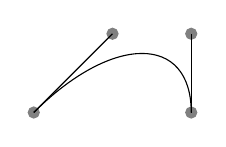
\begin{tikzpicture}
  \filldraw [gray] (0,0) circle (2pt)
  (1,1) circle (2pt)
  (2,1) circle (2pt)
  (2,0) circle (2pt);
  \draw (0,0) .. controls (1,1) and (2,1) .. (2,0);
  \draw (0,0) -- (1,1);
  \draw (2,1) -- (2,0);
\end{tikzpicture}

You can leave out the \keyword{and} (second control point), which causes the first one to be used twice.



\subsection{Circle path}
\label{sec:circle-path}

\begin{lstlisting}
\draw (0,0) circle (10pt);
\end{lstlisting}


\begin{tikzpicture}
  \draw (0,0) circle (10pt);
\end{tikzpicture}



\begin{lstlisting}
\draw (0,0) ellipse (20pt and 10pt);
\end{lstlisting}


\begin{tikzpicture}
  \draw (0,0) ellipse (20pt and 10pt);
\end{tikzpicture}

\subsection{Rectangle path}
\label{sec:rectangle-path}

\begin{lstlisting}
\filldraw [gray] (0,0) circle (2pt);
\filldraw [gray] (0.5,0.5) circle (2pt);
  \draw (0,0) rectangle (0.5,0.5);
\end{lstlisting}


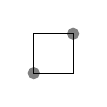
\begin{tikzpicture}
  \filldraw [gray] (0,0) circle (2pt);
  \filldraw [gray] (0.5,0.5) circle (2pt);
  \draw (0,0) rectangle (0.5,0.5);
\end{tikzpicture}

\subsection{Grid path}
\label{sec:grid-path}

\begin{lstlisting}
  \filldraw [gray] (-1.4,-1.4) circle (2pt);
  \filldraw [gray] (1.4,1.4) circle (2pt);

  \draw[step=.5cm,gray,very thin] (-1.4,-1.4) grid (1.4,1.4);
\end{lstlisting}


\begin{tikzpicture}
  \filldraw [gray] (-1.4,-1.4) circle (2pt);
  \filldraw [gray] (1.4,1.4) circle (2pt);

  \draw[step=.5cm,gray,very thin] (-1.4,-1.4) grid (1.4,1.4);
\end{tikzpicture}


\subsection{Arc path}
\label{sec:arc-path}

\begin{lstlisting}
  \filldraw [gray] (0,0) circle (2pt);
  \draw (0mm,0mm) arc (0:30:3cm);
  % (center) arc (angle1:angle2:radius)
  % an arc from angle1 to angle2 on a circle of radius

\end{lstlisting}


\begin{tikzpicture}
  \filldraw [gray] (0,0) circle (2pt);

  \draw (0mm,0mm) arc (0:30:3cm);
  % (center) arc (angle1:angle2:radius)
  % an arc from angle1 to angle2 on a circle of radius
\end{tikzpicture}



\subsection{Clipping a path}
\label{sec:clipping-path}
\begin{lstlisting}
  \draw[step=.5cm,gray,very thin] (-1.4,-1.4) grid (1.4,1.4);
  \draw (-1.5,0) -- (1.5,0);
  \draw (0,-1.5) -- (0,1.5);
  \draw (0,0) circle (1cm);
  \draw (3mm,0mm) arc (0:30:3mm);  

\end{lstlisting}


\begin{tikzpicture}
  \draw[step=.5cm,gray,very thin] (-1.4,-1.4) grid (1.4,1.4);
  \draw (-1.5,0) -- (1.5,0);
  \draw (0,-1.5) -- (0,1.5);
  \draw (0,0) circle (1cm);
  \draw (3mm,0mm) arc (0:30:3mm);  
\end{tikzpicture}

\begin{lstlisting}
  \clip (-0.1,-0.2) rectangle (1.1,0.75);
  \draw[step=.5cm,gray,very thin] (-1.4,-1.4) grid (1.4,1.4);
  \draw (-1.5,0) -- (1.5,0);
  \draw (0,-1.5) -- (0,1.5);
  \draw (0,0) circle (1cm);
  \draw (3mm,0mm) arc (0:30:3mm);  

\end{lstlisting}


\begin{tikzpicture}
  \clip (-0.1,-0.2) rectangle (1.1,0.75);
  \draw[step=.5cm,gray,very thin] (-1.4,-1.4) grid (1.4,1.4);
  \draw (-1.5,0) -- (1.5,0);
  \draw (0,-1.5) -- (0,1.5);
  \draw (0,0) circle (1cm);
  \draw (3mm,0mm) arc (0:30:3mm);  
\end{tikzpicture}

In reality, \keyword{\textbackslash{}draw} is just a shorthand for \keyword{\textbackslash{}path[draw]} and \keyword{\textbackslash{}clip} is a shorthand for \keyword{\textbackslash{}path[clip]} and you could also say \keyword{\textbackslash{}path[draw,clip]}.



\subsection{Filling}
\label{sec:filling}

\begin{lstlisting}
\fill[green!20!white] (0,0) -- (3cm,0cm) arc (0:30:3cm) -- cycle;
\end{lstlisting}


\begin{tikzpicture}
  \fill[green!20!white] (0,0) -- (3cm,0cm) arc (0:30:3cm) -- cycle;
\end{tikzpicture}


The \keyword{--cycle} causes the current path to be closed.


You can also fill and draw a path at the same time using the \keyword{\textbackslash{}filldraw} command.


\subsection{Shading}
\label{sec:shading}

\keyword{\textbackslash{}shade} and \keyword{\textbackslash{}shadedraw} are used for shading and drawing at the same time.

\begin{lstlisting}
  \shade (0,0) rectangle (2,1);
  \shade[top color=yellow,bottom color=black] (3,0) rectangle +(2,1);
  \shade[left color=yellow,right color=black] (6,0) rectangle +(2,1); % relative coordinate
  \shadedraw[inner color=yellow,outer color=black,draw=yellow] (9,0) rectangle +(2,1);
  \shade[ball color=green] (12,.5) circle (.5cm);
\end{lstlisting}


\begin{tikzpicture}
  \shade (0,0) rectangle (2,1);
  \shade[top color=yellow,bottom color=black] (3,0) rectangle +(2,1);
  \shade[left color=yellow,right color=black] (6,0) rectangle +(2,1);
  \shadedraw[inner color=yellow,outer color=black,draw=yellow] (9,0) rectangle +(2,1);
  \shade[ball color=green] (12,.5) circle (.5cm);
\end{tikzpicture}

The default shading is a smooth transition from gray to white. To specify different colors, you can use options.



\subsection{Specifying coordinates}
\label{sec:spec-coord}

\begin{itemize}
\item If you leave out the unites, the default are set to cm and for angle to degree.
\item \keyword{+} means a relative coordinate from the previous specified position and \keyword{++} means a relative coordinate from the previous specified position, making this the new specified position.
\item You can use \keyword{intersection} to specify a coordinate.
\end{itemize}


\begin{lstlisting}
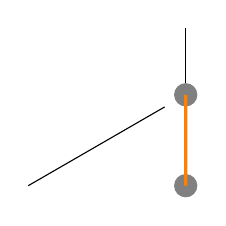
\begin{tikzpicture}[scale=2]
  \draw (1,0) -- (1,1);
  \draw (0,0) -- (30:1cm);
  \filldraw [gray] (1,0) circle (2pt);
  \filldraw [gray] (intersection of 1,0--1,1 and 0,0--30:1cm) circle (2pt);
  \draw[very thick,orange] (1,0) -- (intersection of 1,0--1,1 and 0,0--30:1cm);
\end{tikzpicture}

\end{lstlisting}

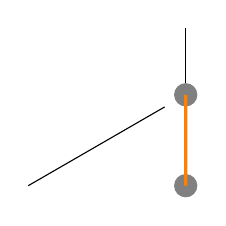
\begin{tikzpicture}[scale=2]
  \draw (1,0) -- (1,1);
  \draw (0,0) -- (30:1cm);
  \filldraw [gray] (1,0) circle (2pt);
  \filldraw [gray] (intersection of 1,0--1,1 and 0,0--30:1cm) circle (2pt);
  \draw[very thick,orange] (1,0) -- (intersection of 1,0--1,1 and 0,0--30:1cm);
\end{tikzpicture}


\subsection{Adding arrow tips}
\label{sec:adding-arrow}


\begin{lstlisting}
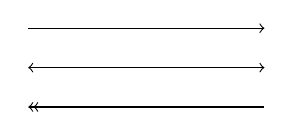
\begin{tikzpicture}
  \draw[->] (-1.5,0) -- (1.5,0);
  \draw[<->] (-1.5,-0.5) -- (1.5,-0.5);
  \draw[<<-] (-1.5,-1) -- (1.5,-1);
\end{tikzpicture}
\end{lstlisting}

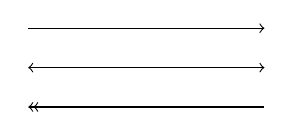
\begin{tikzpicture}
  \draw[->] (-1.5,0) -- (1.5,0);
  \draw[<->] (-1.5,-0.5) -- (1.5,-0.5);
  \draw[<<-] (-1.5,-1) -- (1.5,-1);
\end{tikzpicture}

\begin{lstlisting}
\begin{tikzpicture}[>=stealth]  % >= right arrow tip kind
  \draw[->] (-1.5,0) -- (1.5,0);
\end{tikzpicture}
\end{lstlisting}

\begin{tikzpicture}[>=stealth]  % >= right arrow tip kind
  \draw[->] (-1.5,0) -- (1.5,0);
\end{tikzpicture}



\subsection{Scoping}
\label{sec:scoping}

Scope can let you apply graphic options to a local group.

\begin{lstlisting}
\begin{tikzpicture}[ultra thick]
  \draw (0,0) -- (0,1);
  \begin{scope}[thin]
    \draw (1,0) -- (1,1);
    \draw (2,0) -- (2,1);
  \end{scope}
  \draw (3,0) -- (3,1);
\end{tikzpicture}
\end{lstlisting}

\begin{tikzpicture}[ultra thick]
  \draw (0,0) -- (0,1);
  \begin{scope}[thin]
    \draw (1,0) -- (1,1);
    \draw (2,0) -- (2,1);
  \end{scope}
  \draw (3,0) -- (3,1);
\end{tikzpicture}


\subsection{Transformations}
\label{sec:transformations}

When you specify a coordinate, TikZ applies certain transformations to the given coordinate in order to determine the finally position on the page.

\begin{lstlisting}

\begin{tikzpicture}[even odd rule,rounded corners=2pt,x=10pt,y=10pt]
  % x=10pt set the x unit to 10pt
  \filldraw (0,0)   rectangle (1,1)
  [xshift=5pt,yshift=5pt]   (0,0)   rectangle (1,1)
  [rotate=30]   (-1,-1) rectangle (2,2);

\end{tikzpicture}

\end{lstlisting}


\begin{tikzpicture}[even odd rule,rounded corners=2pt,x=10pt,y=10pt]
  % x=10pt set the x unit to 10pt
  \filldraw (0,0)   rectangle (1,1)
  [xshift=5pt,yshift=5pt]   (0,0)   rectangle (1,1)
  [rotate=30]   (-1,-1) rectangle (2,2);

\end{tikzpicture}

Options to do transformations:
\begin{itemize}
\item \keyword{xshift} and \keyword{yshift}
\item \lstinline|shift={(1,0)}| for shifting to a given point
\item \keyword{rotate} for rotating by a certain angle
\item \keyword{rotate around} for rotating around a given point
\item \keyword{scale} for scaling by a certain factor
\item \keyword{xscale} and \keyword{yscale} (\keyword{xscale=-1} is a flip)
\item \keyword{xslant} and \keyword{yslant} for slanting
\end{itemize}



\subsection{For-loops}
\label{sec:loops}
PGF introduces a command called \keyword{\textbackslash{}foreach}.
The general syntax is
\begin{lstlisting}
\foreach variable in {list of values} command
\end{lstlisting}

\begin{lstlisting}

\begin{tikzpicture}
  \foreach \x in {1,2,...,5,7,9,...,12}
    \foreach \y in {1,...,5}
    {
      \draw (\x,\y) +(-.5,-.5) rectangle ++(.5,.5);
    }
\end{tikzpicture}

\end{lstlisting}


\begin{tikzpicture}
  \foreach \x in {1,2,...,5,7,9,...,12}
    \foreach \y in {1,...,5}
    {
      \draw (\x,\y) +(-.5,-.5) rectangle ++(.5,.5);
    }
\end{tikzpicture}

If you provide two numbers before the \keyword{...}, the \keyword{\textbackslash{}foreach} statement will use their difference for the stepping.




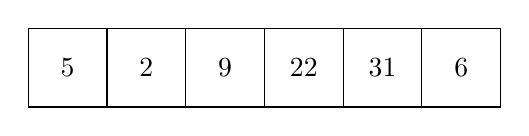
\begin{tikzpicture}
  \foreach \x\y in {0/5,1/2,2/9,3/22,4/31,5/6}
  {
    \node [rectangle,draw,minimum size=1cm] () at (\x ,0) {\y};
  }
\end{tikzpicture}

\begin{lstlisting}

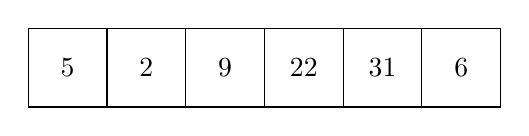
\begin{tikzpicture}
  \foreach \x\y in {0/5,1/2,2/9,3/22,4/31,5/6}
  {
    \node [rectangle,draw,minimum size=1cm] () at (\x ,0) {\y};
  }
\end{tikzpicture}
\end{lstlisting}
\subsection{Adding text}
\label{sec:adding-text}

\begin{lstlisting}
\begin{tikzpicture}
  \draw (0,0) -- node[above=1pt] {above=1pt} (3,0)
  (0,-1) -- node[anchor=north] {anchor=north} (3,-1);
  \draw (0,-3) .. controls (6,-2) and (9,-2) ..
  node[near start,sloped,above] {near start}
  node {midway}
  node[very near end,sloped,below] {very near end} (12,-3);
\end{tikzpicture}
\end{lstlisting}


\begin{tikzpicture}
  \draw (0,0) -- node[above=1pt] {above=1pt} (3,0)
  (0,-1) -- node[anchor=north] {anchor=north} (3,-1);
  \draw (0,-3) .. controls (6,-2) and (9,-2) ..
  node[near start,sloped,above] {near start}
  node {midway}
  node[very near end,sloped,below] {very near end} (12,-3);
\end{tikzpicture}

When TikZ is constructing a path and encounters the keyword \keyword{node} in the middle of a path, it reads a ``node specification''.
The keyword \keyword{node} is typically followed by some options and then some text between curly braces.
This text is put inside a normal TEX box.
All nodes are drawn only after the path has been completely drawn.
You can determine the direction to the position with the \keyword{anchor} option.
And there are simplified writing for the \keyword{anchor} option.
\keyword{below} does the same as \keyword{anchor=south east}.
You can also position labels on curves and, by adding the \keyword{sloped} option, have them rotated such that they match the line’s slope.

\subsection{Load library packages}
\label{sec:load-libr-pack}

\begin{lstlisting}
\usetikzlibrary{arrows,snakes,backgrounds}
\end{lstlisting}




\subsection{Set style}
\label{sec:set-style}

For some commonly used setting, you can set a short name for this setting to save typing and improve clarity.
\begin{lstlisting}
\tikzstyle{place}=[circle,draw=blue!50,fill=blue!20,thick, inner sep=0pt,minimum size=6mm]

\begin{tikzpicture}
  \node [place]  (waiting 1) at (0,2) {};
\end{tikzpicture}
\end{lstlisting}


\subsection{Set color}
\label{sec:set-color}

\begin{lstlisting}
\colorlet{anglecolor}{green!50!black}
\colorlet{sincolor}{red}

\filldraw[fill=green!20,draw=anglecolor] (0,0) -- (3mm,0pt) arc(0:30:3mm);
\end{lstlisting}


\subsection{Local definition}
\label{sec:local-definition}

\begin{lstlisting}
\def\costhirty{0.8660256}
\end{lstlisting}
\subsection{Node}
\label{sec:node}



A node have a \argument{position} and can have a \argument{shape} and \argument{name}.


The \funcword{\textbackslash{}node} command is an abbreviation for \funcword{\textbackslash{}path node}.

\begin{lstlisting}
% shape (circle), style (blue!50,fill=blue!20,thick), size (inner sep=0pt,minimum size=6mm)
\tikzstyle{place}=[circle,draw=blue!50,fill=blue!20,thick,
                   inner sep=0pt,minimum size=6mm]
\tikzstyle{transition}=[rectangle,draw=black!50,fill=black!20,thick,
                        inner sep=0pt,minimum size=4mm]
\begin{tikzpicture}
  % option   name   coordinate  text
  \node[place]      (waiting 1)      at ( 0,2) {};
  \node[place]      (critical 1)     at ( 0,1) {};
  \node[place]      (semaphore)      at ( 0,0) {};
  \node[transition] (leave critical) at ( 1,1) {};
  \node[transition] (enter critical) at (-1,1) {};
\end{tikzpicture}
\end{lstlisting}



% shape (circle), style (blue!50,fill=blue!20,thick), size (inner sep=0pt,minimum size=6mm)
\tikzstyle{place}=[circle,draw=blue!50,fill=blue!20,thick,
                   inner sep=0pt,minimum size=6mm]
\tikzstyle{transition}=[rectangle,draw=black!50,fill=black!20,thick,
                        inner sep=0pt,minimum size=4mm]
\begin{tikzpicture}
  % option   name   coordinate  text
  \node[place]      (waiting 1)      at ( 0,2) {};
  \node[place]      (critical 1)     at ( 0,1) {};
  \node[place]      (semaphore)      at ( 0,0) {};
  \node[transition] (leave critical) at ( 1,1) {};
  \node[transition] (enter critical) at (-1,1) {};
\end{tikzpicture}





We can use relative coordinates and add label to a node.
\begin{lstlisting}
\begin{tikzpicture}
  \tikzstyle{every label}=[red]
  \node[place]   (waiting)      {};                      
  \node[place]   (critical)     [below of=waiting]  {};  
  \node[place]   (semaphore)    [below of=critical,      
                                label=above:$s\le3$] {};   

  \node[transition] (leave critical) [right of=critical] {};
  \node[transition] (enter critical) [left of=critical]  {};
\end{tikzpicture}
\end{lstlisting}


\begin{tikzpicture}
  \tikzstyle{every label}=[red]
  \node[place]   (waiting)      {};                      
  \node[place]   (critical)     [below of=waiting]  {};  
  \node[place]   (semaphore)    [below of=critical,      
                                label=above:$s\le3$] {};   

  \node[transition] (leave critical) [right of=critical] {};
  \node[transition] (enter critical) [left of=critical]  {};
\end{tikzpicture}


We can use \keyword{edge} to draw connection lines.
\begin{lstlisting}
\tikzstyle{pre}=[<-,shorten <=1pt,>=stealth,semithick]
\tikzstyle{post}=[->,shorten >=1pt,>=stealth,semithick]
\begin{tikzpicture}[bend angle=45]
  \node[place]    (waiting)                            {};
  \node[place]    (critical)       [below of=waiting]  {};
  \node[place]    (semaphore)      [below of=critical] {};

  \node[transition] (leave critical) [right of=critical] {}
  edge [pre]                                 (critical)
  edge [post,bend right] node[auto,swap] {2} (waiting)
  edge [pre, bend left]                      (semaphore);
  \node[transition] (enter critical) [left of=critical]  {}
  edge [post]                              (critical) 
  edge [pre, bend left]                    (waiting)
  edge [post,bend right]                   (semaphore);
\end{tikzpicture}
\end{lstlisting}

\tikzstyle{pre}=[<-,shorten <=1pt,>=stealth,semithick]
\tikzstyle{post}=[->,shorten >=1pt,>=stealth,semithick]
\begin{tikzpicture}[bend angle=45]
  \node[place]    (waiting)                            {};
  \node[place]    (critical)       [below of=waiting]  {};
  \node[place]    (semaphore)      [below of=critical] {};

  \node[transition] (leave critical) [right of=critical] {}
  edge [pre]                                 (critical)
  edge [post,bend right] node[auto,swap] {2} (waiting)
  edge [pre, bend left]                      (semaphore);
  \node[transition] (enter critical) [left of=critical]  {}
  edge [post]                              (critical) 
  edge [pre, bend left]                    (waiting)
  edge [post,bend right]                   (semaphore);
\end{tikzpicture}



\subsection{Snake line}
\label{sec:snake-line}
\usetikzlibrary{snakes}
\begin{tikzpicture}
  \draw [->,snake=snake,
         segment amplitude=.4mm,
         segment length=2mm,
         line after snake=1mm] (0,0) -- (3,0);
\end{tikzpicture}


\begin{lstlisting}

\begin{tikzpicture}
  \draw [->,snake=snake,
         segment amplitude=.4mm,
         segment length=2mm,
         line after snake=1mm] (0,0) -- (3,0);
\end{tikzpicture}
\end{lstlisting}
\section{Examples}
\label{sec:examples}

\subsection{A picture for Karl’s students}
\label{sec:pict-karls-stud}

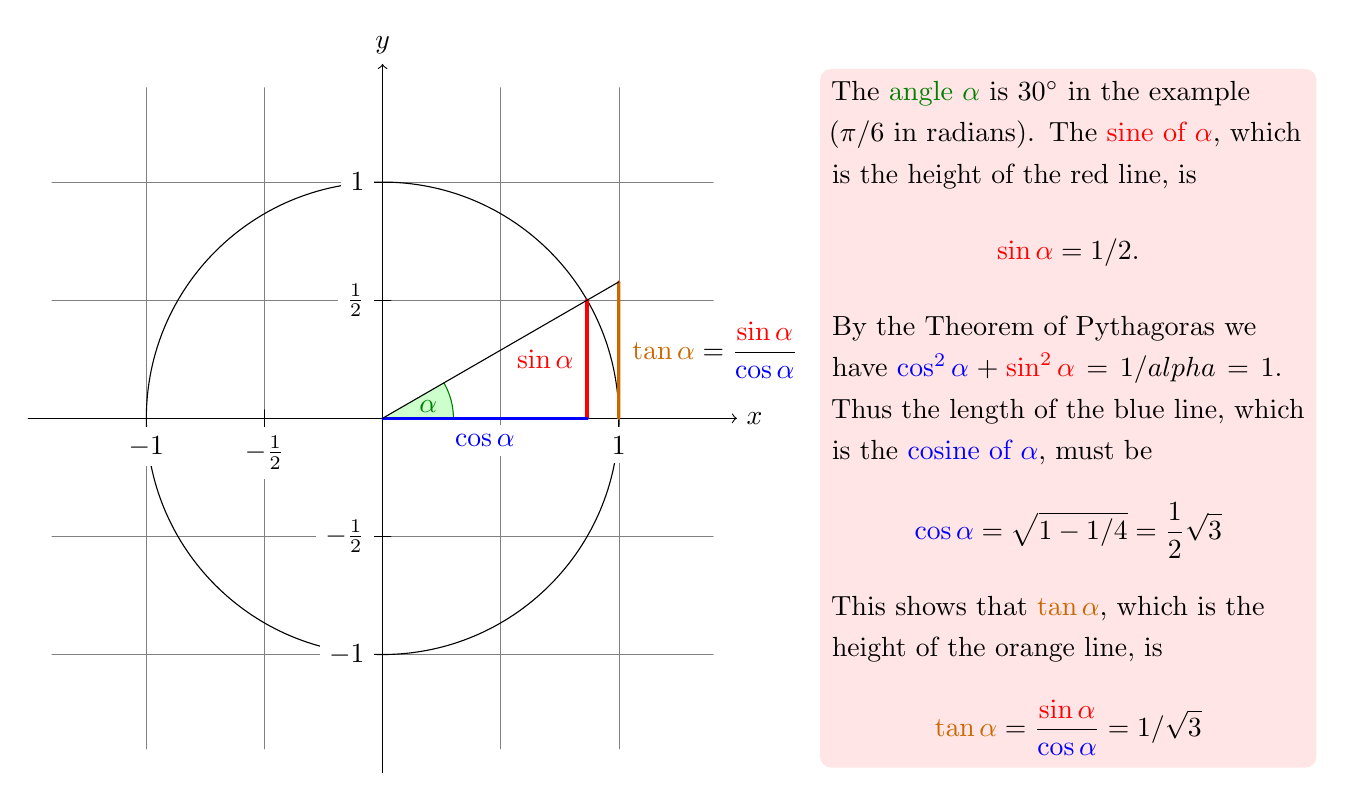
\begin{tikzpicture}[scale=3,cap=round]
  % Local definitions
  \def\costhirty{0.8660256}
  % Colors
  \colorlet{anglecolor}{green!50!black}
  \colorlet{sincolor}{red}
  \colorlet{tancolor}{orange!80!black}
  \colorlet{coscolor}{blue}
  % Styles
  \tikzstyle{axes}=[]
  \tikzstyle{important line}=[very thick]
  \tikzstyle{information text}=[rounded corners,fill=red!10,inner sep=1ex]
  % The graphic
  \draw[style=help lines,step=0.5cm] (-1.4,-1.4) grid (1.4,1.4);
  \draw (0,0) circle (1cm);
  \begin{scope}[style=axes]
    \draw[->] (-1.5,0) -- (1.5,0) node[right] {$x$} coordinate(x axis);
    \draw[->] (0,-1.5) -- (0,1.5) node[above] {$y$} coordinate(y axis);
    \foreach \x/\xtext in {-1, -.5/-\frac{1}{2}, 1}
    \draw[xshift=\x cm] (0pt,1pt) -- (0pt,-1pt) node[below,fill=white] {$\xtext$};
    \foreach \y/\ytext in {-1, -.5/-\frac{1}{2}, .5/\frac{1}{2}, 1}
    \draw[yshift=\y cm] (1pt,0pt) -- (-1pt,0pt) node[left,fill=white] {$\ytext$};
  \end{scope}
  \filldraw[fill=green!20,draw=anglecolor] (0,0) -- (3mm,0pt) arc(0:30:3mm);
  \draw (15:2mm) node[anglecolor] {$\alpha$};
  \draw[style=important line,sincolor]
  (30:1cm) -- node[left=1pt,fill=white] {$\sin \alpha$} (30:1cm |- x axis);
  \draw[style=important line,coscolor]
  (30:1cm |- x axis) -- node[below=2pt,fill=white] {$\cos \alpha$} (0,0);
  \draw[style=important line,tancolor] (1,0) -- node[right=1pt,fill=white] {
    $\displaystyle \tan \alpha \color{black}=
    \frac{{\color{sincolor}\sin \alpha}}{\color{coscolor}\cos \alpha}$}
  (intersection of 0,0--30:1cm and 1,0--1,1) coordinate (t);
  \draw (0,0) -- (t);
  \draw[xshift=1.85cm]
  node[right,text width=6cm,style=information text]
  {
    The {\color{anglecolor} angle $\alpha$} is $30^\circ$ in the
      example ($\pi/6$ in radians). The {\color{sincolor}sine of
        $\alpha$}, which is the height of the red line, is
      \[
      {\color{sincolor} \sin \alpha} = 1/2.
      \]

      By the Theorem of Pythagoras we have ${\color{coscolor}\cos ^2 \alpha}+{\color{sincolor} \sin^{2} \alpha} = 1/alpha=1$.
      Thus the length of the blue line, which is the {\color{coscolor} cosine of $\alpha$}, must be
    $$
    {\color{coscolor}\cos \alpha}=\sqrt{1-1 / 4}=\frac{1}{2} \sqrt{3}
    $$
    This shows that {\color{tancolor}$\tan \alpha$}, which is the height of the orange line, is
    $$
    {\color{tancolor}\tan \alpha}=\frac{\color{sincolor}\sin \alpha}{\color{coscolor}\cos \alpha}=1 / \sqrt{3}
    $$
  };
\end{tikzpicture}

\begin{lstlisting}
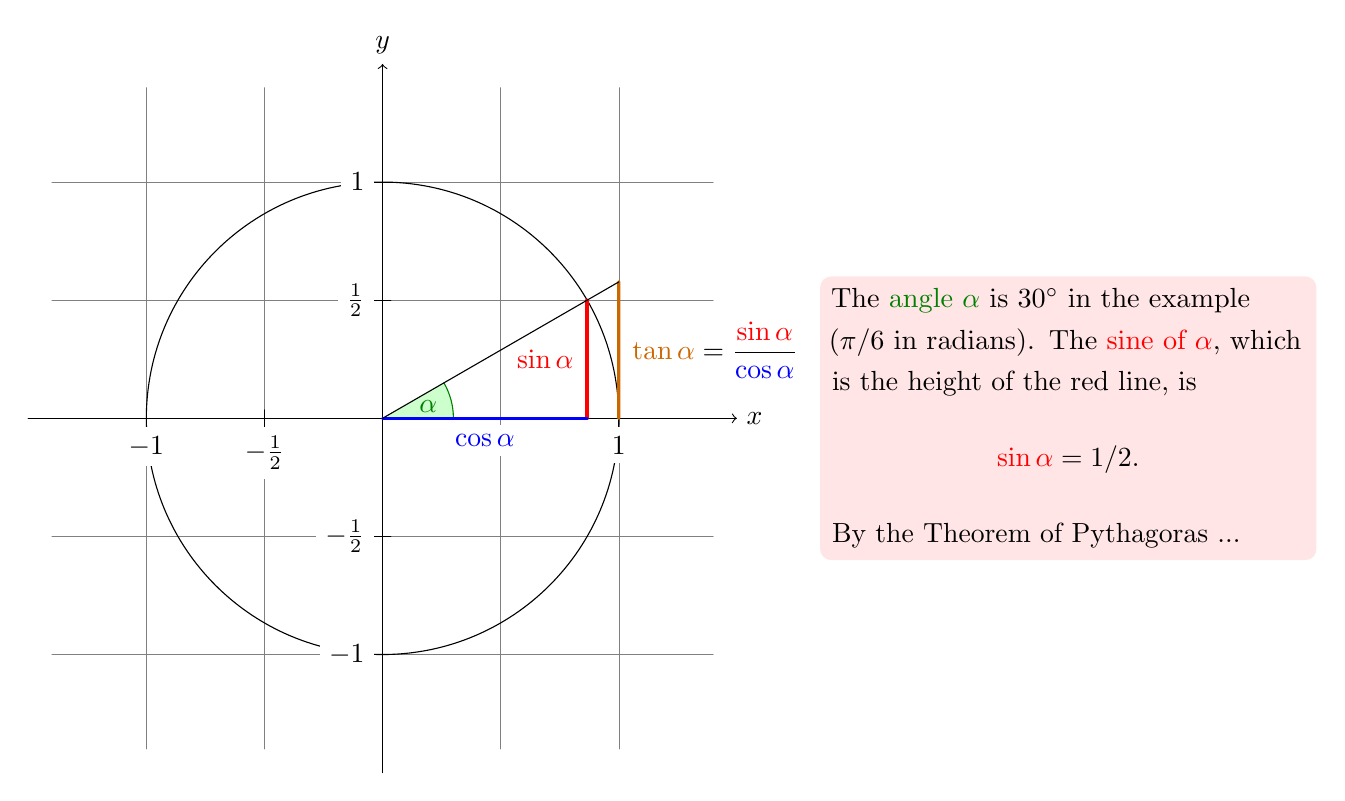
\begin{tikzpicture}[scale=3,cap=round]
% Local definitions
  \def\costhirty{0.8660256}
% Colors
  \colorlet{anglecolor}{green!50!black}
  \colorlet{sincolor}{red}
  \colorlet{tancolor}{orange!80!black}
  \colorlet{coscolor}{blue}
% Styles
  \tikzstyle{axes}=[]
  \tikzstyle{important line}=[very thick]
  \tikzstyle{information text}=[rounded corners,fill=red!10,inner sep=1ex]
% The graphic
  \draw[style=help lines,step=0.5cm] (-1.4,-1.4) grid (1.4,1.4);
  \draw (0,0) circle (1cm);
  \begin{scope}[style=axes]
    \draw[->] (-1.5,0) -- (1.5,0) node[right] {$x$} coordinate(x axis);
    \draw[->] (0,-1.5) -- (0,1.5) node[above] {$y$} coordinate(y axis);
    \foreach \x/\xtext in {-1, -.5/-\frac{1}{2}, 1}
      \draw[xshift=\x cm] (0pt,1pt) -- (0pt,-1pt) node[below,fill=white] {$\xtext$};
    \foreach \y/\ytext in {-1, -.5/-\frac{1}{2}, .5/\frac{1}{2}, 1}
      \draw[yshift=\y cm] (1pt,0pt) -- (-1pt,0pt) node[left,fill=white] {$\ytext$};
\end{scope}
  \filldraw[fill=green!20,draw=anglecolor] (0,0) -- (3mm,0pt) arc(0:30:3mm);
  \draw (15:2mm) node[anglecolor] {$\alpha$};
  \draw[style=important line,sincolor]
    (30:1cm) -- node[left=1pt,fill=white] {$\sin \alpha$} (30:1cm |- x axis);
  \draw[style=important line,coscolor]
    (30:1cm |- x axis) -- node[below=2pt,fill=white] {$\cos \alpha$} (0,0);
  \draw[style=important line,tancolor] (1,0) -- node[right=1pt,fill=white] {
    $\displaystyle \tan \alpha \color{black}=
    \frac{{\color{sincolor}\sin \alpha}}{\color{coscolor}\cos \alpha}$}
    (intersection of 0,0--30:1cm and 1,0--1,1) coordinate (t);
  \draw (0,0) -- (t);
  \draw[xshift=1.85cm]
    node[right,text width=6cm,style=information text]
    {
      The {\color{anglecolor} angle $\alpha$} is $30^\circ$ in the
      example ($\pi/6$ in radians). The {\color{sincolor}sine of
        $\alpha$}, which is the height of the red line, is
      \[
      {\color{sincolor} \sin \alpha} = 1/2.
      \]
      By the Theorem of Pythagoras ...
    };
\end{tikzpicture}
\end{lstlisting}



\subsection{A Petri-Net for Hagen}
\label{sec:petri-net-hagen}

\usetikzlibrary{arrows,snakes,backgrounds}

\tikzstyle{place}=[circle,draw=blue!50,fill=blue!20,thick,inner sep=0pt,minimum size=6mm]
\tikzstyle{transition}=[rectangle,draw=black!50,fill=black!20,thick,inner sep=0pt,minimum size=4mm]

\tikzstyle{pre}=[<-,shorten <=1pt,>=stealth,semithick]
\tikzstyle{post}=[->,shorten >=1pt,>=stealth,semithick]

\tikzstyle{every place}=[minimum size=6cm,thick,draw=blue!75,fill=blue!20]
\tikzstyle{every transition}=[thick,draw=black!75,fill=black!20]
\tikzstyle{red place}=[place,draw=red!75,fill=red!20]
\tikzstyle{every label}=[red]


\begin{tikzpicture}[node distance=1.3cm,>=stealth,bend angle=45,auto]
  \node [place] (w1)  {};
  \node [place] (c1) [below of=w1] {};
  \node [place] (s) [below of=c1,label=above:\(s\le 3\)] {};
  \node [place] (c2) [below of=s] {};
  \node [place] (w2) [below of=c2] {};

  \node [transition] (e1) [left of=c1] {}
  edge [pre,bend left] (w1)
  edge [post,bend right] (s)
  edge [post] (c1);
  \node [transition] (e2) [left of=c2] {}
  edge [pre, bend right] (w2)
  edge [pre, bend left] (s)
  edge [post] (c2);
  \node [transition] (l1) [right of=c1] {}
  edge [pre] (c1)
  edge [pre,bend left] (s)
  edge [post,bend right] node [swap] {2} (w1);
  \node [transition] (l2) [right of=c2] {}
  edge [pre] (c2)
  edge [pre,bend right] (s)
  edge [post,bend left] node {2} (w2);

  \begin{scope}[xshift=6cm]
    \node [place] (w1') {};
    \node [place] (c1') [below of=w1'] {};
    \node [red place] (s1') [below of=c1',xshift=-0.5cm] [label=left:\(s\)] {};
    \node [red place] (s2') [below of=c1',xshift=0.5cm] [label=right:\(\bar s\)] {};
    \node [place] (c2') [below of=s1',xshift=.5cm] {};
    \node [place] (w2') [below of=c2'] {};

    \node [transition] (e1') [left of=c1'] {}
    edge [pre,bend left] (w1')
    edge [post] (s1')
    edge [pre] (s2')
    edge [post] (c1');
    \node [transition] (e2') [left of=c2'] {}
    edge [pre,bend right] (w2')
    edge [post] (s1')
    edge [pre] (s2')
    edge [post] (c2');
    \node [transition] (l1') [right of=c1'] {}
    edge [pre] (c1')
    edge [pre] (s1')
    edge [post] (s2')
    edge [post,bend right] node [swap]  {2} (w1');
    \node [transition] (l2') [right of=c2'] {}
    edge [pre] (c2')
    edge [pre] (s1')
    edge [post] (s2')
    edge [post,bend left] node {2} (w2');
  \end{scope}

  \draw [-to,thick,snake=snake,segment amplitude=.4mm,segment length=2mm,line after snake=1mm]
    ([xshift=5mm]s -| l1) -- ([xshift=-5mm]s1' -| e1')
    node [above=1mm,midway,text width=3cm,text centered]
      {replacement of the \textcolor{red}{capacity} by \textcolor{red}{two places}};
  \begin{pgfonlayer}{background}
    \filldraw [line width=4mm,join=round,black!10]
      (w1.north  -| l1.east)  rectangle (w2.south  -| e1.west)
      (w1'.north -| l1'.east) rectangle (w2'.south -| e1'.west);
  \end{pgfonlayer}
\end{tikzpicture}


\begin{lstlisting}
\usetikzlibrary{arrows,snakes,backgrounds}

\tikzstyle{place}=[circle,draw=blue!50,fill=blue!20,thick,inner sep=0pt,minimum size=6mm]
\tikzstyle{transition}=[rectangle,draw=black!50,fill=black!20,thick,inner sep=0pt,minimum size=4mm]

\tikzstyle{pre}=[<-,shorten <=1pt,>=stealth,semithick]
\tikzstyle{post}=[->,shorten >=1pt,>=stealth,semithick]

\tikzstyle{every place}=[minimum size=6cm,thick,draw=blue!75,fill=blue!20]
\tikzstyle{every transition}=[thick,draw=black!75,fill=black!20]
\tikzstyle{red place}=[place,draw=red!75,fill=red!20]
\tikzstyle{every label}=[red]


\begin{tikzpicture}[node distance=1.3cm,>=stealth,bend angle=45,auto]
  \node [place] (w1)  {};
  \node [place] (c1) [below of=w1] {};
  \node [place] (s) [below of=c1,label=above:\(s\le 3\)] {};
  \node [place] (c2) [below of=s] {};
  \node [place] (w2) [below of=c2] {};

  \node [transition] (e1) [left of=c1] {}
  edge [pre,bend left] (w1)
  edge [post,bend right] (s)
  edge [post] (c1);
  \node [transition] (e2) [left of=c2] {}
  edge [pre, bend right] (w2)
  edge [pre, bend left] (s)
  edge [post] (c2);
  \node [transition] (l1) [right of=c1] {}
  edge [pre] (c1)
  edge [pre,bend left] (s)
  edge [post,bend right] node [swap] {2} (w1);
  \node [transition] (l2) [right of=c2] {}
  edge [pre] (c2)
  edge [pre,bend right] (s)
  edge [post,bend left] node {2} (w2);

  \begin{scope}[xshift=6cm]
    \node [place] (w1') {};
    \node [place] (c1') [below of=w1'] {};
    \node [red place] (s1') [below of=c1',xshift=-0.5cm] [label=left:\(s\)] {};
    \node [red place] (s2') [below of=c1',xshift=0.5cm] [label=right:\(\bar s\)] {};
    \node [place] (c2') [below of=s1',xshift=.5cm] {};
    \node [place] (w2') [below of=c2'] {};

    \node [transition] (e1') [left of=c1'] {}
    edge [pre,bend left] (w1')
    edge [post] (s1')
    edge [pre] (s2')
    edge [post] (c1');
    \node [transition] (e2') [left of=c2'] {}
    edge [pre,bend right] (w2')
    edge [post] (s1')
    edge [pre] (s2')
    edge [post] (c2');
    \node [transition] (l1') [right of=c1'] {}
    edge [pre] (c1')
    edge [pre] (s1')
    edge [post] (s2')
    edge [post,bend right] node [swap]  {2} (w1');
    \node [transition] (l2') [right of=c2'] {}
    edge [pre] (c2')
    edge [pre] (s1')
    edge [post] (s2')
    edge [post,bend left] node {2} (w2');
  \end{scope}

  \draw [-to,thick,snake=snake,segment amplitude=.4mm,segment length=2mm,line after snake=1mm]
    ([xshift=5mm]s -| l1) -- ([xshift=-5mm]s1' -| e1')
    node [above=1mm,midway,text width=3cm,text centered]
      {replacement of the \textcolor{red}{capacity} by \textcolor{red}{two places}};
  \begin{pgfonlayer}{background}
    \filldraw [line width=4mm,join=round,black!10]
      (w1.north  -| l1.east)  rectangle (w2.south  -| e1.west)
      (w1'.north -| l1'.east) rectangle (w2'.south -| e1'.west);
  \end{pgfonlayer}
\end{tikzpicture}

\end{lstlisting}
%%% Local Variables:
%%% mode: latex
%%% TeX-master: "latex"
%%% End:


\chapter{Reference}
\label{cha:reference}

\begin{lstlisting}
% \usepackage{amssymb}
\checkmark{}
\end{lstlisting}
\checkmark{}
%%% Local Variables:
%%% mode: latex
%%% TeX-master: "latex"
%%% End:



% Pages are numbered with Arabic numbers.
% Chapters generate a table of contents entry but don't get a number.
\backmatter
\nocite{*}
\bibliographystyle{alpha}
\bibliography{tex}

\clearpage{}
% just setting an anchor like \hypertarget{}{}
% fix the problem that anchor point to the previous section
\phantomsection                 
\printindex{}
\end{document}

%%% Local Variables:
%%% mode: latex
%%% TeX-master: t
%%% End:



\chapter{Version Control}
\label{cha:version-control}



A version control system gives you automated help at keeping a change history for a file or group of files.
It allows you to recover any stage in that history, and it makes getting reports on the differences between versions easy.


Here we use Git as the version control system.
In Emacs, we use Magit.
Magit is an interface to the version control system Git, implemented as an Emacs package.


\section{Installation}
\label{sec:installation-1}
In you \argument{.emacs} or \argument{.emacs.el} file, add the following code.

\begin{lstlisting}
;; Use package manager interface.
(require 'package)

;; Add melpa site to package archives.
;; This is used define where to fetch package. 
(add-to-list 'package-archives '("melpa-stable" . "https://stable.melpa.org/packages/") t)

;; Load Emacs Lisp packages, and activate them.
(package-initialize)


;; Install Magit
(package-install 'magit)
\end{lstlisting}

\section{Basic}
\label{sec:basic}

\subsection{Show Status Buffer}
\label{sec:show-status-buffer}


Type \keyword{C-x g} to display information about the current Git repository in a dedicated buffer, called the status buffer. If the current directory isn’t located within a Git repository, then prompt for an existing repository or an arbitrary directory, depending on option ``magit-repository-directories'', and show the status of the selected repository instead.

\begin{itemize}
\item If that option specifies any existing repositories, then offer those for completion and show the status buffer for the selected one.
\item Otherwise read an arbitrary directory using regular file-name completion.  If the selected directory is the top-level of an existing working tree, then show the status buffer for that.
\item Otherwise offer to initialize the selected directory as a new repository.  After creating the repository show its status buffer.
\end{itemize}

Depending on what state your repository is in, this buffer may contain sections titled ``Staged changes'', ``Unstaged changes'', ``Unmerged into origin/master'', ``Unpushed to origin/master'', and many others.

Move between sections using \keyword{p} and \keyword{n}.
Note that the bodies of some sections are hidden.
Type \keyword{TAB} to expand or collapse the section at point.
You can also use \keyword{C-tab} to cycle the visibility of the current section and its children. 

\begin{tcolorbox}
  In status buffer, remember use \keyword{C-h m} to get help information about this mode.
\end{tcolorbox}


\subsection{Stage and Unstage}
\label{sec:stage-unstage}

Move to a file section inside the section named ``Unstaged changes'' and type \keyword{s} to stage the changes you have made to that file.
That file now appears under ``Staged changes''.

Magit can stage and unstage individual hunks, not just complete files.
Move to the file you have just staged, expand it using \keyword{TAB}, move to one of the hunks using \keyword{n}, and unstage just that by typing \keyword{u}.
Note how the staging (\keyword{s}) and unstaging (\keyword{u}) commands operate on the change at point.
Many other commands behave the same way.


You can also un-/stage just part of a hunk.
Inside the body of a hunk section (move there using \keyword{C-n}), set the mark using \keyword{C-SPC} and move down until some added and/or removed lines fall inside the region but not all of them.
Again type \keyword{s} to stage.

It is also possible to un-/stage multiple files at once.
Move to a file section, type \keyword{C-SPC}, move to the next file using \keyword{n}, and then \keyword{s} to stage both files.

\subsection{Commit}
\label{sec:commit}

If you want to commit your changes.
Type \keyword{c}.
This shows the available commit commands and arguments in a buffer at the bottom of the frame.
Each command and argument is prefixed with the key that invokes/sets it.
If you want to create a ``normal'' commit, just type \keyword{c} again.


Now two new buffers appear.
One is for writing the commit message, the other shows a diff with the changes that you are about to commit.
Write a message and then type \keyword{C-c C-c} to actually create the commit.

\subsection{Push}
\label{sec:push}

You can push it by typing \keyword{p} to show all the available push commands and arguments and then \keyword{p} to push to a branch with the same name as the local branch onto the remote configured as the push-remote.
If the push-remote is not configured yet, then you would first be prompted for the remote to push to.


\subsection{Transient prefix commands}
\label{sec:help}

To show a menu that lists all menus, type \keyword{h}.
(Such menus are also called ``transient prefix commands'' or just ``transients''.)

\keyword{C-x M-g} is the global binding of this menu.
You can invoke this menu even not in status buffer.
In file visiting buffers \keyword{C-c M-g} brings up a similar menu featuring commands that act on just the visited file.

\begin{figure}[!htbp]
  \centering
  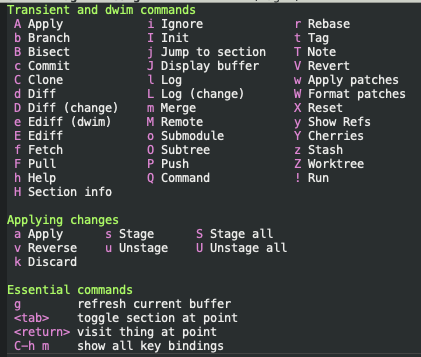
\includegraphics[width=\textwidth]{transient-commands}
  \caption{Transient prefix commands}
  \label{fig:transient-commands}
\end{figure}

\newpage{}
\subsection{Summary}
\label{sec:summary}

\begin{table}[H]
  \centering
  \begin{tabular}{>{\bfseries}lp{0.6\textwidth}}
    \toprule
    \head{Binding} & \head{Meaning} \\
    \midrule
    C-x g & Show the status of the current Git repository in a buffer.\\
    TAB & expand or hide the section at point.\\
    C-TAB & Cycle the visibility of the current section and its children.\\
    RET & visit the change or commit at point\\
    n & Move to the beginning of the next visible section.\\
    p & Move to the beginning of the current or the previous visible section.\\
    s & stage\\
    u & unstage\\
    c & commit\\
    p & push\\
    h & invoke major commands\\
    C-x M-g & invoke major commands\\
    C-c M-g & invoke major commands that act on just the visited file\\
    \bottomrule
  \end{tabular}
  \caption{Basic magit commands}
  \label{tab:basic-magit-commands}
\end{table}





% Here are some commands used in status buffer shown in Table \ref{tab:magit-cmds}.
% \begin{center}
%   \begin{longtable}[H]{>{\bfseries}lp{0.6\textwidth{}}}
      %       \toprule
      %       \head{Binding} & \head{Meaning}\\
      %       \midrule
      %       \endfirsthead

      %       \toprule
      %       \head{Binding} & \head{Meaning}\\
      %       \midrule
      %       \endhead

      %       \midrule
      %       \multicolumn{2}{c}{{Continued on next page}}\\
      %       \bottomrule
      %       \endfoot

      %       \endlastfoot

      %       \midrule
      %       SPC & Either show the commit or stash at point in the appropriate buffer, or if that buffer is already being displayed in the current frame and contains information about that commit or stash, then instead scroll the buffer up.  If there is no commit or stash at point, then prompt for a commit.\\
      %       ! & Run git or another command, or launch a graphical utility.\\
      %       \$ & Display the current repository’s process buffer.\\
      %       \% & Act on a worktree.\\
      %       + & Increase the context for diff hunks by COUNT(\keyword{C-u n}) lines.\\
      %       - & Decrease the context for diff hunks by COUNT(\keyword{C-u n}) lines.\\
      %       0 & Reset context for diff hunks to the default height.\\
      %       1 & Show surrounding sections on first level.\\
      %       2 & Show surrounding sections up to second level.\\
      %       3 & Show surrounding sections up to third level.\\
      %       4 & Show surrounding sections up to fourth level.\\
      %       : & Execute COMMAND asynchronously; display output.\\
      %       < & Move point to the beginning of the buffer.\\
      %       > & Move point to the end of the buffer.\\
      %       \bottomrule
      %       \caption{Magit commands\label{tab:magit-cmds}}
      %     \end{longtable}
      %       \end{center}

\section{Interface Concepts}
\label{sec:interface-concepts}

\subsection{Modes and Buffers}
\label{sec:modes-buffers}


Magit provides several major-modes.
For each of these modes there usually exists only one buffer per repository.
Separate modes and thus buffers exist for commits, diffs, logs, and some other things.

Besides these special purpose buffers, there also exists an overview buffer, called the status buffer.
It’s usually from this buffer that the user invokes Git commands, or creates or visits other buffers.


\begin{table}[H]
  \centering
  \begin{tabular}{>{\bfseries}lp{0.6\textwidth}}
    \toprule
    \head{Binding} & \head{Meaning}\\
    \midrule
    q & Bury the current buffer. With a prefix argument, kill the buffer instead. With two prefix arguments, also kill all Magit buffers associated with this repository.\\
    g & Refresh the current buffer if its major mode derives from ``magit-mode'', and refresh the corresponding status buffer.\\
    G & Refreshes all Magit buffers belonging to the current repository and also reverts all unmodified buffers that visit files being tracked in the current repository.\\
    \bottomrule
  \end{tabular}
  \caption{Modes and buffers commands}
  \label{tab:modes-buffers-cmds}
\end{table}

\subsection{Sections}
\label{sec:sections}

Magit buffers are organized into nested sections, which can be collapsed and expanded, similar to how sections are handled in Org mode.
Each section also has a type, and some sections also have a value.
For each section type there can also be a local keymap, shared by all sections of that type.

Taking advantage of the section value and type, many commands operate on the current section, or when the region is active and selects sections of the same type, all of the selected sections.
Commands that only make sense for a particular section type are usually bound in section type keymaps.

\begin{table}[H]
  \centering
  \begin{tabular}{>{\bfseries}lp{0.6\textwidth}}
    \toprule
    \head{Binding} & \head{Meaning}\\
    \midrule
    n & Move to the beginning of the next visible section.\\
    p & Move to the beginning of the current or the previous visible section.\\
    M-p & Move to the beginning of the previous sibling section. If there is no previous sibling section, then move to the parent section instead.\\
    M-n & Move to the beginning of the next sibling section. If there is no next sibling section, then move to the parent section instead.\\
    \textasciicircum{} & Move to the beginning of the parent of the current section.\\
    \midrule
    TAB & Expand or hide the section at point.\\
    C-TAB & Cycle the visibility of current section and its children.\\
    magit-section-cycle-diffs & Cycle the visibility of diff-related sections in the current buffer.\\
    magit-section-cycle-global & Cycle the visibility of all sections in the current buffer.\\
    \midrule
    1 & \multirow{4}{*}{Show sections surrounding the current section up to level N.}\\
    2 & \\
    3 & \\
    4 & \\
    \midrule
    M-1 & \multirow{4}{*}{Show all sections up to level N.}\\
    M-2 & \\
    M-3 & \\
    M-4 & \\
    \midrule
    H & Shows information about the section at point in a separate buffer.\\
    \bottomrule
  \end{tabular}
  \caption{Sections commands}
  \label{tab:sections-cmds}
\end{table}

\subsection{Transient Commands}
\label{sec:transient-commands}

Many Magit commands are implemented as transient commands.
First the user invokes a prefix command, which causes its infix arguments and suffix commands to be displayed in the echo area.
The user then optionally sets some infix arguments and finally invokes one of the suffix commands.


\subsection{Transient Arguments and Buffer Variables}
\label{sec:trans-argum-buff}

The infix arguments of many of Magit’s transient prefix commands cease to have an effect once the git command that is called with those arguments has returned.
Commands that create a commit are a good example for this.
If the user changes the arguments, then that only affects the next invocation of a suffix command.
If the same transient prefix command is later invoked again, then the arguments are initially reset to the default value.
It is possible to cycle through previously used sets of arguments using \keyword{C-M-p} and \keyword{C-M-n}.

\begin{figure}[!htbp]
  \centering
  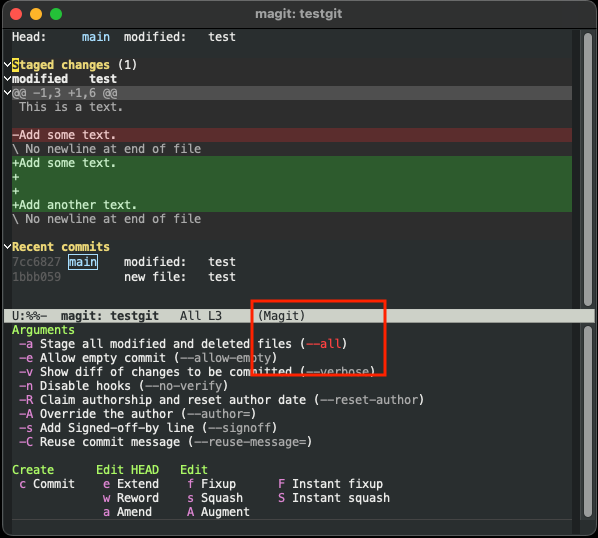
\includegraphics[width=0.7\textwidth]{transient-commit-1}
  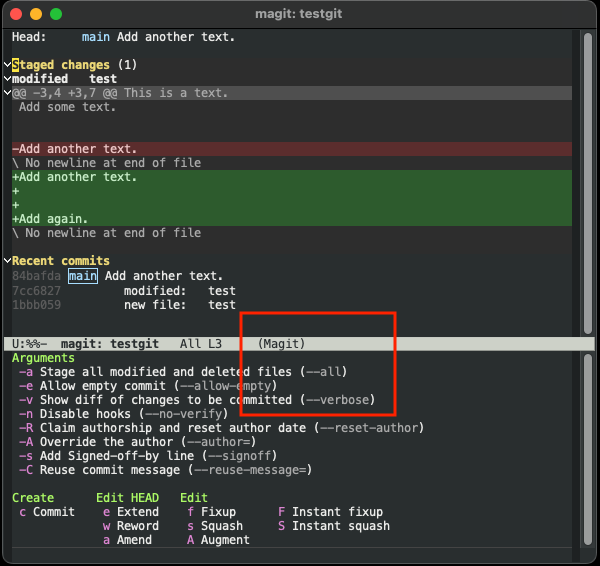
\includegraphics[width=0.7\textwidth]{transient-commit-2}
  \caption{Transient commit arguments}
  \label{fig:transient-commit-arguments}
\end{figure}


Figure \ref{fig:transient-commit-arguments} show this effect.
After the commit, the next time you commit, the argument is reset to the default value.


However the infix arguments of many other transient commands continue to have an effect even after the git command that was called with those arguments has returned.
The most important commands like this are those that display a diff or log in a dedicated buffer.
Their arguments obviously continue to have an effect for as long as the respective diff or log is being displayed.
Furthermore the used arguments are stored in buffer-local variables for future reference.
We can also use \keyword{C-M-p} and \keyword{C-M-n} to previous and next arguments stored in buffer-local variables.


It is also possible to change the diff and log arguments used in the current buffer (including the status buffer, which contains both diff and log sections) using the respective ``refresh'' transient prefix commands on \keyword{D} and \keyword{L}.
(\keyword{d} and \keyword{l} on the other hand are intended to change what diff or log is being displayed.
It is possible to also change how the diff or log is being displayed at the same time, but if you only want to do the latter, then you should use the refresh variants.)
Because these secondary diff and log transient prefixes are about changing the arguments used in the current buffer, they always start out with the set of arguments that are currently in effect in that buffer.

\begin{figure}[!htbp]
  \centering
  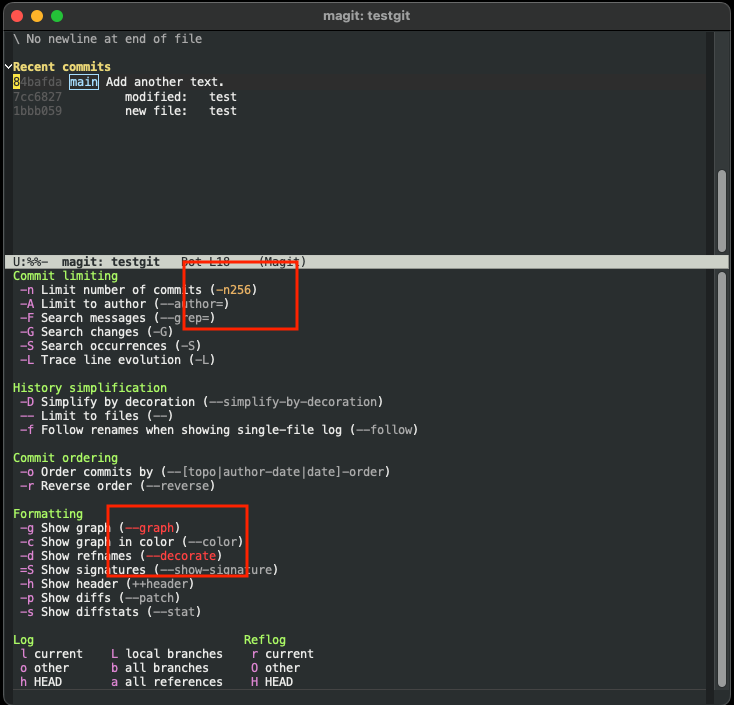
\includegraphics[width=0.8\textwidth]{transient-log}
  \caption{Transient log arguments}
  \label{fig:transient-log-arguments}
\end{figure}

Figure \ref{fig:transient-log-arguments} show this effect.
The arguments are still there.

\subsection{Running Git}
\label{sec:running-git}

Magit runs Git either for side-effects (e.g. when pushing) or to get some value (e.g. the name of the current branch).
When Git is run for side-effects, the process output is logged in a per-repository log buffer, which can be consulted using the \keyword{magit-process} command when things don't go as expected.



\begin{table}[H]
  \centering
  \begin{tabular}{>{\bfseries}lp{0.6\textwidth}}
    \toprule
    \head{Binding} & \head{Meaning}\\
    \midrule
    \$ & Displays the process buffer for the current repository.\\
    k & Kills the process represented by the section at point.\\
    ! & Run git command\\
    \bottomrule
  \end{tabular}
  \caption{Git commands}
  \label{tab:Git-cmds}
\end{table}

\section{Inspecting}
\label{sec:inspecting}

The functionality provided by Magit can be roughly divided into three groups:
\begin{itemize}
\item inspecting existing data
\item manipulating existing data or adding new data
\item transferring data
\end{itemize}


\begin{table}[H]
  \centering
  \begin{tabular}{l>{\bfseries}lp{0.6\textwidth}}
    \toprule
    \head{Group} & \head{Binding} & \head{Meaning}\\
    \midrule
    status & C-x g & Show status buffer.\\
    \midrule
    \multirow{3}{*}{logging} & l & show a commit or reference log.\\
                 & L & Change the arguments used for the log(s) in the current buffer.\\
                 & Y & Show commits that are in a certain branch but that have not been merged in the upstream branch.\\
    \midrule
    \multirow{2}{*}{diffing} & d & Show changes between different versions.\\
                 & D & Change the arguments used for the diff(s) in the current buffer.\\
    \midrule
    \multirow{2}{*}{ediffing} & e & Compare, stage, or resolve using Ediff. This command tries to guess what file, and what commit or range the user wants to compare, stage, or resolve using Ediff.\\
                 & E & Show differences using the Ediff package.\\
    \midrule
    references & y & Lists branches and tags in a dedicated buffer.\\
    \midrule
    bisecting & B & Narrow in on the commit that introduced a bug.\\
    \bottomrule
  \end{tabular}
  \caption{Inspecting Commands}
  \label{tab:inspecting-commands}
\end{table}


\newpage{}

\section{Manipulating}
\label{sec:manipulating}


\begin{table}[H]
  \centering
  \begin{tabular}{l>{\bfseries}lp{0.6\textwidth}}
    \toprule
    \head{Group} & \head{Binding} & \head{Meaning}\\      
    \midrule
    init & I & Initialize a repository and then shows the status buffer for the new repository.\\
    \midrule
    clone & C & Clone a repository.\\
    \midrule
    \multirow{2}{*}{staging} & s & Add the change at point to the staging area.\\
                 & S & Stage all changes to files modified in the worktree.\\
    \midrule
    \multirow{2}{*}{unstaging} & u & Remove the change at point from the staging area.\\
                 & U & Remove all changes from the staging area.\\
    \midrule
    \multirow{3}{*}{applying} & a & Apply the change at point to the working tree.\\
    & k & Remove the change at point from the working tree.\\
    & v & Reverse the change at point in the working tree.\\
    \midrule
    commit & c & Reverse the change at point in the working tree.\\
    \midrule
    branching & b & Add, configure or remove a branch.\\
    \midrule
    merging & m & Merge branches.\\
    \midrule
    rebasing & r & Transplant commits and/or modify existing commits.\\
    \midrule
    \multirow{2}{*}{cherry picking} & A & Apply or transplant commits.\\
                 & V & Revert existing commits, with or without creating new commits.\\
    \midrule
    resetting & x & Reset the HEAD and index to some commit read from the user and defaulting to the commit at point, and possibly also reset the working tree. With a prefix argument reset the working tree otherwise don't.\\
                 & X & Reset the HEAD and index to some commit read from the user and defaulting to the commit at point. The working tree is kept as-is.\\
    \midrule
    stashing & z & Stash uncommitted changes.\\
    \midrule
    \midrule
    tag & t & Create or delete a tag.\\
    \midrule
    note & T & Edit notes attached to commits.\\
    \midrule
    submodules & o & Act on a submodule.\\
    \midrule
    subtree & O & Import or export subtrees.\\
    \midrule
    worktree & Z & Act on a worktree.\\
    \bottomrule
  \end{tabular}
  \caption{Manipulating commands}
  \label{tab:manipulating-cmds}
\end{table}


\section{Transferring}
\label{sec:transferring}

\begin{table}[H]
  \centering
  \begin{tabular}{l>{\bfseries}lp{0.6\textwidth}}
    \toprule
    \head{Group} & \head{Binding} & \head{Meaning}\\      
    \midrule
    remote & M & Add, configure or remove a remote.\\
    \midrule
    fetching & f & Fetch from repository.\\
    \midrule
    pulling & F & Pull from repository.\\
    \midrule
    pushing & P & Push to repository.\\
    \midrule
    \multirow{2}{*}{patches} & W & Create or apply patches.\\
                 & w & Apply patches received by email.\\
    \bottomrule
  \end{tabular}
  \caption{Manipulating commands}
  \label{tab:manipulating-cmds}
\end{table}


%%% Local Variables:
%%% mode: latex
%%% TeX-master: "emacs"
%%% End:


\chapter{Org}
\label{cha:org}


Org is a mode for keeping notes, maintaining TODO lists, and project planning with a fast and effective plain-text markup language.
It also is an authoring system with unique support for literate programming and reproducible research.
Org is implemented on top of Outline mode.

Files with the '.org' extension use Org mode by default.





\section{Document Structure}
\label{sec:document-structure}


\subsection{Headlines}
\label{sec:headlines-1}


Headlines define the structure of an outline tree.
Org headlines start on the left margin with one or more stars followed by a space.

\begin{tcolorbox}
\begin{verbatim}
* Top level headline
** Second level
*** Third level
    some text
*** Third level
    more text
* Another top level headline
\end{verbatim}
\end{tcolorbox}

\subsection{Motion}
\label{sec:motion}


\begin{table}[H]
  \centering
  \begin{tabular}{>{\bfseries}ll}
    \toprule
    \head{Binding} & \head{Meaning}\\
    \midrule
    C-c C-n & Next heading\\
    C-c C-p & Previous heading\\
    C-c C-f & Next heading same level\\
    C-c C-b & Previous heading same level\\
    C-c C-u & Backward to higher level heading.\\
    \bottomrule
  \end{tabular}
  \caption{Motion commands}
  \label{tab:org-motion-cmds}
\end{table}



\subsection{Visibility Cycling}
\label{sec:visibility-cycling}

Outlines make it possible to hide parts of the text in the buffer.
Org uses just two commands, bound to \keyword{TAB} and \keyword{S-TAB} to change the visibility in the buffer.




\begin{table}[H]
  \centering
  \begin{tabular}{>{\bfseries}lp{0.6\textwidth}}
    \toprule
    \head{Binding} & \head{Meaning}\\
    \midrule
    TAB & Rotate current subtree among ``fold - children - subtree''. Point must be on a headline for this to work.\\
    S-TAB & Rotate the entire buffer among ``overview - content - show all''\\
    C-c C-r & Reveal context around point, showing the current entry, the following heading and the hierarchy above.\\
    C-c C-k & Expose all the headings of the subtree, but not their bodies.\\
    C-c TAB & Expose all direct children of the subtree. With a numeric prefix argument N, expose all children down to level N.\\
    C-c C-x b & Show the current subtree in an indirect buffer\\
    \bottomrule
  \end{tabular}
  \caption{Visibility cycling commands}
  \label{tab:visibility-cycling-cmds}
\end{table}

\newpage{}
\subsection{Structure Editing}
\label{sec:structure-editing}

\begin{table}[H]
  \centering
  \begin{tabular}{>{\bfseries}lp{0.6\textwidth}}
    \toprule
    \head{Binding} & \head{Meaning}\\
    \midrule
    M-RET & Insert a new heading, item or row.\\
    C-RET & Insert a new heading at the end of the current subtree.\\
    M-S-RET & Insert new TODO entry with same level as current heading.\\
    TAB & In a new entry with no text yet, the first TAB demotes the entry to become a child of the previous one. The next TAB makes it a parent, and so on, all the way to top level. Yet another TAB, and you are back to the initial level.\\
    M-\(\leftarrow\) & Promote current heading by one level.\\
    M-\(\rightarrow\) & Demote current heading by one level\\
    M-S-\(\leftarrow\) & Promote the current subtree by one level.\\
    M-S-\(\rightarrow\) & Demote the current subtree by one level.\\
    M-\(\uparrow\) & Move subtree up, i.e., swap with previous subtree of same level.\\
    M-\(\downarrow\) & Move subtree down, i.e., swap with next subtree of same level.\\
    C-c @ & Mark the subtree at point. Hitting repeatedly marks subsequent subtrees of the same level as the marked subtree.\\
    C-c C-x C-w & Kill subtree, i.e., remove it from buffer but save in kill ring. With a numeric prefix argument N, kill N sequential subtrees.\\
    C-c C-x M-w & Copy subtree to kill ring. With a numeric prefix argument N, copy the N sequential subtrees.\\
    C-c C-x C-y & Yank subtree from kill ring. This does modify the level of the subtree to make sure the tree fits in nicely at the yank position. \\
    C-c C-w & Move the entry or entries at point to another heading.\\
    C-c \textasciicircum{} & Sort same-level entries. When there is an active region, all entries in the region are sorted. Otherwise the children of the current headline are sorted. \\
    C-x n s & Narrow buffer to current subtree.\\
    C-x n b & Narrow buffer to current block.\\
    C-x n w & Widen buffer to remove narrowing.\\
    C-c * & Turn a normal line or plain list item into a headline—so that it becomes a subheading at its location.\\
    \bottomrule
  \end{tabular}
  \caption{Structure editing commands}
  \label{tab:structure-editing-cmds}
\end{table}



\subsection{Sparse Tree}
\label{sec:sparse-tree}


An important feature of Org mode is the ability to construct \keyword{sparse trees} for selected information in an outline tree, so that the entire document is folded as much as possible, but the selected information is made visible along with the headline structure above it.

\begin{table}[H]
  \centering
  \begin{tabular}{>{\bfseries}ll}
    \toprule
    \head{Binding} & \head{Meaning}\\
    \midrule
    C-c / & This prompts for an extra key to select a sparse-tree creating command.\\
    M-g n or M-g M-n & Jump to the next sparse tree match in this buffer.\\
    M-g p or M-g M-p & Jump to the previous sparse tree match in this buffer.\\
    \bottomrule
  \end{tabular}
  \caption{Sparse tree commands }
  \label{tab:sparse-tree-cmds}
\end{table}

\subsection{Drawers}
\label{sec:drawers}

Sometimes you want to keep information associated with an entry, but you normally do not want to see it.
For this, Org mode has \keyword{drawers}.
They can contain anything but a headline and another drawer.
Drawers look like this:

\begin{tcolorbox}
\begin{verbatim}
** This is a headline
Still outside the drawer
:DRAWERNAME:
This is inside the drawer.
:END:
After the drawer.
\end{verbatim}
\end{tcolorbox}


You can interactively insert a drawer at point by typing \keyword{C-c C-x d}.
With an active region, this command puts the region inside the drawer.
With a prefix argument, this command creates a 'PROPERTIES' drawer right below the current headline.
Org mode uses this special drawer for storing properties.
You cannot use it for anything else.


Visibility cycling on the headline hides and shows the entry, but keep the drawer collapsed to a single line.
In order to look inside the drawer, you need to move point to the drawer line and press \keyword{TAB} there.

\subsection{Block}
\label{sec:block}

Org mode uses \keyword{\#+BEGIN … \#+END} blocks for various purposes from including source code examples to capturing time logging information.
These blocks can be folded and unfolded by pressing TAB in the \keyword{\#+BEGIN} line. 

\section{Plain Lists}
\label{sec:plain-lists}

Org knows ordered lists, unordered lists, and description lists.
\begin{itemize}
\item Unordered list items start with \keyword{-, + } or \keyword{*} as bullets.
\item Ordered list items start with a numeral followed by either a period or a right parenthesis, such as \keyword{1.} or \keyword{1)}. If you want a list to start with a different value — e.g., 10 — start the text of the item with \keyword{[@10]}
\item Description list items are unordered list items, and contain the separator \keyword{::} to distinguish the description term from the description.
\end{itemize}

The following commands act on items when point is in the first line of an item—the line with the bullet or number.
Some of them imply the application of automatic rules to keep list structure intact.
If some of these actions get in your way, configure \argument{org-list-automatic-rules} to disable them individually.



\begin{table}[H]
  \centering
  \begin{tabular}{>{\bfseries}lp{0.6\textwidth}}
    \toprule
    \head{Binding} & \head{Meaning}\\
    \midrule
    TAB & Items can be folded  or unfolded\\
    M-RET & Insert new item at current level.\\
    M-S-RET & Insert a new item with a checkbox\\
    M-\(\uparrow\) or M-\(\downarrow\) & Move the item including subitems up/down.\\
    M-\(\leftarrow\) or M-\(\rightarrow\) & Decrease/increase the indentation of an item, leaving children alone.\\
    M-S-\(\leftarrow\) or M-S-\(\rightarrow\) & Decrease/increase the indentation of the item, including subitems.\\
    C-c C-c & If there is a checkbox in the item line, toggle the state of the checkbox.\\
    C-c \# & Update the statistic cookie in the current outline entry.\\    
    C-c - &  Cycle the entire list level through the different itemize/enumerate bullets .\\
    C-c * & Turn a plain list item into a headline.\\
    C-c C-* & Turn the whole plain list into a subtree of the current heading.\\
    C-c \textasciicircum{} & Sort the plain list.\\
    \bottomrule
  \end{tabular}
  \caption{Plain list commands}
  \label{tab:plain-list-cmds}
\end{table}


\subsection{Checkboxes}
\label{sec:checkboxes}

Every item in a plain list can be made into a checkbox by starting it with the string \keyword{[ ]}.
This feature is similar to TODO items, but is more lightweight.
Checkboxes are not included into the global TODO list, so they are often great to split a task into a number of simple steps.


\begin{verbatim}

* light task [25%]
  - [-] task 1 [33%]
    - [X] task 1-1
    - [ ] task 1-2
    - [ ] task 1-3
  - [X] task 2
  - [ ] task 3
  - [ ] task 4

\end{verbatim}

\section{Hyperlinks}
\label{sec:hyperlinks}

\subsection{Link Format}
\label{sec:link-format}


The general link format looks like this:
\begin{tcolorbox}
\begin{verbatim}
[[LINK][DESCRIPTION]]
or alternatively
[[LINK]]
\end{verbatim}
\end{tcolorbox}

Once a link in the buffer is complete, with all brackets present, Org changes the display so that \keyword{DESCRIPTION} is displayed instead of \keyword{[[LINK][DESCRIPTION]]} and \keyword{LINK} is displayed instead of \keyword{[[LINK]]}.
You can directly edit the visible part of a link.
This can be either the LINK part, if there is no description, or the DESCRIPTION part otherwise.
To also edit the invisible LINK part, use \keyword{C-c C-l} with point on the link.


\subsection{Internal Links}
\label{sec:internal-links}

A link that does not look like a URL—i.e., does not start with a known scheme or a file name—refers to the current document.
You can follow it with \keyword{C-c C-o} when point is on the link.

Org provides several refinements to internal navigation within a document.
Most notably, a construct like \keyword{\lstinline|[[\#my-custom-id]]|} specifically targets the entry with the \keyword{CUSTOM\_ID} property set to \keyword{my-custom-id}.
Also, an internal link looking like \keyword{\lstinline|[[*Some section]]|} points to a headline with the name \keyword{Some section}.


When the link does not belong to any of the cases above, Org looks for a dedicated target: the same string in double angular brackets, like \keyword{\textless{}\textless{}My Target\textgreater{}\textgreater{}}.

If no dedicated target exists, the link tries to match the exact name of an element within the buffer.


Following a link pushes a mark onto Org’s own mark ring.
You can return to the previous position with \textgreater{C-c \&}.
Using this command several times in direct succession goes back to positions recorded earlier.


\subsection{External Links}
\label{sec:external-links}

External links are URL-like locators.
They start with a short identifying string followed by a colon.
There can be no space after the colon.


Here is the part set of built-in link types:
\begin{itemize}[itemsep=10pt]
\item file\\
  File links. File name may be remote, absolute, or relative.
  Additionally, you can specify a line number, or a text search.
  In Org files, you may link to a headline name, a custom ID, or a code reference instead.
  \verb|file:/home/li/notebook/emacs/emacs.tex|.
\item attachment\\
  Same as file links but for files and folders attached to the current node.
  Attachment links are intended to behave exactly as file links but for files relative to the attachment directory.
  \verb|attachment:projects.org|.
\item docview\\
  Link to a document opened with DocView mode.
  You may specify a page number.\\
  \verb|docview:papers/last.pdf|.
\item doi\\
  Link to an electronic resource, through its handle.
  \verb|doi:10.1000/182|.
\item elisp\\
  Execute an Elisp command upon activation.
  \verb|elisp:(find-file "~/notebook")|.
\item http\\
  \verb|http://www.google.com|.
\item https\\
  \verb|https://www.google.com|.
\item mailto\\
  Link to message composition.
  \verb|mailto:mingmingli916@gmail.com|.
\item shell\\
  Execute a shell command upon activation.
  \verb|shell:date|.
\end{itemize}




\subsection{Handling Links}
\label{sec:handling-links}

\begin{lrbox}{\lstbox}
\begin{lstlisting}[language=elisp, basicstyle=\footnotesize]
(global-set-key (kbd "C-c l") #'org-store-link)
\end{lstlisting}
\end{lrbox}

Org provides methods to create a link in the correct syntax, to insert it into an Org file, and to follow the link.
The main function is \argument{org-store-link} (\keyword{C-c l})\footnote{\usebox{\lstbox}}.
It stores a link to the current location. The link is stored for later insertion into an Org buffer.
The kind of link that is created depends on the current buffer:
\begin{itemize}
\item Org mode buffers\\
  For Org files, if there is a \keyword{\textless{}\textless{}target\textgreater{}\textgreater{}} at point, the link points to the target.
  Otherwise it points to the current headline.
  If the headline has a \keyword{CUSTOM\_ID} property, store a link to this custom ID.
\item Other files\\
  For any other file, the link points to the file, with a search string pointing to the contents of the current line.
  If there is an active region, the selected words form the basis of the search string.
\item Agenda view\\
  The created link points to the entry referenced by the current line.
\end{itemize}

\subsection{Link Abbreviations}
\label{sec:link-abbreviations}

Long URL can be cumbersome to type, and often many similar links are needed in a document.
For this you can use link abbreviations.
An abbreviated link looks like this:
\begin{verbatim}
[[linkword:tag][description]]
\end{verbatim}
where the tag is optional.
Abbreviations are resolved according to the information in the variable \argument{org-link-abbrev-alist} that relates the linkwords to replacement text.
\begin{lstlisting}[language=elisp]
(setq org-link-abbrev-alist
      '(("google" . "https://www.google.com")))
\end{lstlisting}
If the replacement text contains the string \keyword{\%s}, it is replaced with the tag.
Using \keyword{\%(my-function)} passes the tag to a custom Lisp function, and replace it by the resulting string.


\subsection{Search Options in File Links}
\label{sec:search-options-file}

File links can contain additional information to make Emacs jump to a particular location in the file when following a link. This can be a line number or a search option after a double colon.

\begin{verbatim}
[[file:~/code/main.c::255]]
[[file:~/xx.org::My Target]]
[[file:~/xx.org::*My Target]]
[[file:~/xx.org::#my-custom-id]]
[[file:~/xx.org::/regexp/]]
[[attachment:main.c::255]]
\end{verbatim}

\subsection{Summary}
\label{sec:summary-1}


\begin{lrbox}{\lstbox}
\begin{lstlisting}[language=elisp, basicstyle=\footnotesize]
(with-eval-after-load 'org
  (define-key org-mode-map (kbd "M-n") #'org-next-link)
  (define-key org-mode-map (kbd "M-p") #'org-previous-link))
\end{lstlisting}
\end{lrbox}

\begin{table}[H]
  \centering
  \begin{tabular}{>{\bfseries}lp{0.6\textwidth}}
    \toprule
    \head{Binding} & \head{Meaning}\\
    \midrule
    C-c C-l & Insert a link. With a \keyword{C-u} prefix, prompts for a file to link to. When point is on an existing link, edit the link and description parts of the link.\\
    C-c C-o & Open the link when point is on the link.\\
    C-c \% & Push the current position onto the Org mark ring, to be able to return easily.\\
    C-c \& & Following a link pushes a mark onto Org’s own mark ring. You can return to the previous position with this command.\\
    M-n & Move forward to the next link in the buffer.\tablefootnote{This is achieved by:\par\usebox{\lstbox}}\\
    M-p & Move backward to the previous link in the buffer.\\
    \bottomrule
  \end{tabular}
  \caption{Hyperlinks command summary}
  \label{tab:hyperlinks-cmds}
\end{table}

\section{TODO items}
\label{sec:todo-items}

Org mode does not maintain \keyword{TODO} lists as separate documents1.
Instead, TODO items are an integral part of the notes file, because TODO items usually come up while taking notes!
With Org mode, simply mark any entry in a tree as being a TODO item.

\subsection{Basic TODO Functionality}
\label{sec:basic-todo-funct}

Any headline becomes a TODO item when it starts with the word \keyword{TODO}.


\begin{table}[H]
  \centering
  \begin{tabular}{>{\bfseries}ll}
    \toprule
    \head{Binding} & \head{Meaning}\\
    \midrule
    C-c C-t & Roate the TODO state of the current item.\\
    S-\(\rightarrow\) S-\(\leftarrow\) & Select the following/preceding TODO state.\\
    S-M-RET & Insert a new TODO entry below the current one.\\
    \bottomrule
  \end{tabular}
  \caption{Basic TODO commands}
  \label{tab:basic-todo-cmds}
\end{table}

\subsection{Extended Use of TODO Keywords}
\label{sec:extended-use-todo}

By default, marked TODO entries have one of only two states: TODO and DONE.
Org mode allows you to classify TODO items in more complex ways with TODO keywords (stored in \keyword{org-todo-keywords}).


The structure of Org files makes it easy to define TODO dependencies.
Usually, a parent TODO task should not be marked as done until all TODO subtasks, or children tasks, are marked as done.
Sometimes there is a logical sequence to (sub)tasks, so that one subtask cannot be acted upon before all siblings above it have been marked as done.
If you customize the variable \argument{org-enforce-todo-dependencies}, Org blocks entries from changing state to DONE while they have TODO children that are not DONE. Furthermore, if an entry has a property \keyword{ORDERED}, each of its TODO children is blocked until all earlier siblings are marked as done.

\begin{table}[H]
  \centering
  \begin{tabular}{>{\bfseries}lp{0.6\textwidth}}
    \toprule
    \head{Binding} & \head{Meaning}\\
    \midrule
    C-c C-x o & Toggle the 'ORDERED' property of the current entry.\\
    \bottomrule
  \end{tabular}
  \caption{Extended TODO commands}
  \label{tab:extended-todo-cmds}
\end{table}


\subsection{Progress Logging}
\label{sec:progress-logging}

\begin{table}[H]
  \centering
  \begin{tabular}{>{\bfseries}lp{0.6\textwidth}}
    \toprule
    \head{Binding} & \head{Meaning}\\
    \midrule
    C-u C-c C-t & Prompt for a note and record the time of the TODO state change\\
    \bottomrule
  \end{tabular}
  \caption{Progress logging commands}
  \label{tab:progress-logging-commands}
\end{table}


\subsection{Priorities}
\label{sec:priorities}

Prioritizing can be done by placing a \keyword{priority cookie} into the headline of a TODO item right after the TODO keyword, like this:
\begin{verbatim}
* TODO [#A] Summarize org mode
\end{verbatim}

By default, Org mode supports three priorities: ‘A’, ‘B’, and ‘C’.
‘A’ is the highest priority.
An entry without a cookie is treated as equivalent if it had priority ‘B’.
Priorities make a difference only for sorting in the agenda.
Outside the agenda, they have no inherent meaning to Org mode.


Priorities can be attached to any outline node; they do not need to be TODO items.

\begin{table}[H]
  \centering
  \begin{tabular}{>{\bfseries}lp{0.6\textwidth}}
    \toprule
    \head{Binding} & \head{Meaning}\\
    \midrule
    C-c , & Set the priority of the current headline. The command prompts for a priority character ‘A’, ‘B’ or ‘C’. When you press SPC instead, the priority cookie, if one is set, is removed from the headline.\\
    S-\(\uparrow\) & Increase the priority of the current headline.\\
    S-\(\downarrow\) & Decrease the priority of the current headline.\\
    \bottomrule
  \end{tabular}
  \caption{}
  \label{tab:}
\end{table}

\subsection{Breaking Down Tasks into Subtasks}
\label{sec:breaking-down-tasks}

It is often advisable to break down large tasks into smaller, manageable subtasks.
You can do this by creating an outline tree below a TODO item, with detailed subtasks on the tree.
To keep an overview of the fraction of subtasks that have already been marked as done, insert either \keyword{[/]} or \keyword{[\%]} anywhere in the headline.
These cookies are updated each time the TODO status of a child changes, or when pressing C-c C-c on the cookie.



\section{Dates and Times}
\label{sec:dates-times}


To assist project planning, TODO items can be labeled with a date and/or a time.
The specially formatted string carrying the date and time information is called a \keyword{timestamp} in Org mode.

\subsection{Timestamps}
\label{sec:timestamps}

A timestamp is a specification of a date in a special format.
A timestamp can appear anywhere in the headline or body of an Org tree entry.
Its presence causes entries to be shown on specific dates in the agenda.


There are the following timestamps:
\begin{itemize}
\item Plain timestamp\\
  A simple timestamp just assigns a date/time to an item.
\begin{verbatim}
<2022-11-07 Mon 14:00>
\end{verbatim}
\item Timestamp with repeater interval\\
  A timestamp may contain a \keyword{repeater interval}, indicating that it applies not only on the given date, but again and again after a certain interval of N days (d), weeks (w), months (m), or years (y).
\begin{verbatim}
<2022-11-07 Mon 7:00 +1d>
\end{verbatim}
\item Diary-style expression entries\\
  For more complex date specifications, Org mode supports using the special expression diary entries implemented in the Emacs Calendar package.
\begin{verbatim}
<%%(diary-float t 4 2)>
\end{verbatim}
\item Time/Data range\\
  Two timestamps connected by \keyword{-{}-} denote a range.
\begin{verbatim}
<2022-11-07 Mon>--<2022-11-08 Tue>
\end{verbatim}
\item Inactive timestamp\\
  Just like a plain timestamp, but with square brackets instead of angular ones.
  These timestamps are inactive in the sense that they do not trigger an entry to show up in the agenda.
\begin{verbatim}
[2022-11-07 Mon]
\end{verbatim}
\end{itemize}


\subsection{Creating Timestamps}
\label{sec:creating-timestamps}

For Org mode to recognize timestamps, they need to be in the specific format. All commands listed in Table \ref{tab:creating-timestamp-cmds} produce timestamps in the correct format.

\begin{table}[H]
  \centering
  \begin{tabular}{>{\bfseries}lp{0.6\textwidth{}}}
    \toprule
    \head{Binding} & \head{Meaning}\\
    \midrule
    C-c . & Prompt for a date and insert a corresponding timestamp. When point is at an existing timestamp in the buffer, the command is used to modify this timestamp. When this command is used twice in succession, a time range is inserted.\\
    C-u C-c . & Use the alternative format which contains date and time.\\
    C-u C-u C-c . & Insert an active timestamp with the current time without prompting.\\
    C-c ! & Like C-c ., but insert an inactive timestamp that does not cause an agenda entry.\\
    C-c C-c & Normalize timestamp, insert or fix day name if missing or wrong.\\
    C-c < & Insert a timestamp corresponding to point date in the calendar.\\
    C-c > & Access the Emacs calendar for the current date. If there is a timestamp in the current line, go to the corresponding date instead.\\
    C-c C-o & Access the agenda for the date given by the timestamp or -range at point.\\
    S-\(\leftarrow\) or S-\(\rightarrow\) & Change date at point by one day\\
    S-\(\uparrow\) or S-\(\downarrow\) & On the beginning or enclosing bracket of a timestamp, change its type. Within a timestamp, change the item under point. Point can be on a year, month, day, hour or minute. When the timestamp contains a time range like ‘15:30-16:30’, modifying the first time also shifts the second, shifting the time block with constant length. To change the length, modify the second time. \\
    C-c C-y & Evaluate a time range by computing the difference between start and end. With a prefix argument, insert result after the time range.\\ 

    \bottomrule
  \end{tabular}
  \caption{Creating timestamp commands}
  \label{tab:creating-timestamp-cmds}
\end{table}

When Org mode prompts for a date/time, the default is shown in default date/time format, and the prompt therefore seems to ask for a specific format.
But it in fact accepts date/time information in a variety of formats.
Generally, the information should start at the beginning of the string.
Org mode finds whatever information is in there and derives anything you have not specified from the \keyword{default date and time}.
The default is usually the current date and time, but when modifying an existing timestamp, or when entering the second stamp of a range, it is taken from the stamp in the buffer.
When filling in information, Org mode assumes that most of the time you want to enter a date in the future: if you omit the month/year and the given day/month is before today, it assumes that you mean a future date.


For example, let’s assume that today is June 13, 2006.
\begin{verbatim}
‘3-2-5’                =>  2003-02-05                            
‘2/5/3’                =>  2003-02-05                            
‘14’                   =>  2006-06-14                            
‘12’                   =>  2006-07-12                            
‘2/5’                  =>  2007-02-05                            
‘Fri’                  =>  nearest Friday (default date or later)
‘sep 15’               =>  2006-09-15                            
‘feb 15’               =>  2007-02-15                            
‘sep 12 9’             =>  2009-09-12                             
‘12:45’                =>  2006-06-13 12:45                       
‘22 sept 0:34’         =>  2006-09-22 0:34                        
‘w4’                   =>  ISO week for of the current year 2006  
‘2012 w4 fri’          =>  Friday of ISO week 4 in 2012           
‘2012-w04-5’           =>  Same as above                          
\end{verbatim}



Furthermore you can specify a relative date by giving, as the first thing in the input: a plus/minus sign, a number and a letter—‘h’, ‘d’, ‘w’, ‘m’ or ‘y’—to indicate a change in hours, days, weeks, months, or years.
With ‘h’ the date is relative to the current time, with the other letters and a single plus or minus, the date is relative to today at 00:00.
With a double plus or minus, it is relative to the default date.
If instead of a single letter, you use the abbreviation of day name, the date is the Nth such day.

\begin{verbatim}
‘+0’         =>  today
‘.’          =>  today
‘+2h’        =>  two hours from now
‘+4d’        =>  four days from today
‘+4’         =>  same as +4d
‘+2w’        =>  two weeks from today
‘++5’        =>  five days from default date
‘+2tue’      =>  second Tuesday from now
\end{verbatim}

Parallel to the minibuffer prompt, a calendar is popped up.
You can control the calendar fully from the minibuffer:
\begin{table}[H]
  \centering
  \begin{tabular}{>{\bfseries}lp{0.6\textwidth}}
    \toprule
    \head{Binding} & \head{Meaning}\\
    \midrule
    RET & Choose date at point in calendar.\\
    S-\(\rightarrow\) & One day forward.\\
    S-\(\leftarrow\) & One day backward.\\
    S-\(\downarrow\) & One week forward.\\
    S-\(\uparrow\) & One week backward.\\
    M-S-\(\rightarrow\) & One month forward.\\
    M-S-\(\leftarrow\) & One month backward.\\
    > & Scroll calendar forward by one month.\\
    < & Scroll calendar backward by one month.\\
    C-v & Scroll calendar forward by 3 months.\\
    M-v & Scroll calendar backward by 3 months.\\
    C-. & Select today's date.\\
    \bottomrule
  \end{tabular}
  \caption{Minibuffer commands}
  \label{tab:minibuffer-cmds}
\end{table}

\subsection{Deadlines and Scheduling}
\label{sec:deadlines-scheduling}

A timestamp may be preceded by special keywords to facilitate planning.
Both the timestamp and the keyword have to be positioned immediately after the task they refer to.


\begin{itemize}[itemsep=10pt]
\item \keyword{DEADLINE}\\
\begin{verbatim}
* TODO Task
  DEADLINE: <2022-11-07 Mon>
\end{verbatim}
\item \keyword{SCHEDULED}\\
\begin{verbatim}
* TODO Task
  SCHEDULED: <2022-11-07 Mon>
\end{verbatim}
\end{itemize}



\begin{table}[H]
  \centering
  \begin{tabular}{>{\bfseries}ll}
    \toprule
    \head{Binding} & \head{Meaning}\\
    \midrule
    C-c C-d & Insert \keyword{DEADLINE} keyword along with a stamp.\\
    C-c C-s & Insert \keyword{SCHEDULED} keyword along with a stamp.\\
    \bottomrule
  \end{tabular}
  \caption{}
  \label{tab:}
\end{table}

\subsubsection{Repeated tasks}
\label{sec:repeated-tasks}

Some tasks need to be repeated again and again.
Org mode helps to organize such tasks using a so-called \keyword{repeater} in a ‘DEADLINE’, ‘SCHEDULED’, or plain timestamps.
\begin{verbatim}
** TODO Pay the rent
   DEADLINE: <2022-11-07 Mon +1m>
\end{verbatim}

the \keyword{+1m} is a repeater; the intended interpretation is that the task has a deadline on ‘<2022-11-07>’ and repeats itself every (one) month starting from that time.
You can use yearly, monthly, weekly, daily and hourly repeat cookies by using the ‘y’, ‘m’, ‘w’, ‘d’ and ‘h’ letters.
If you need both a repeater and a special warning period in a deadline entry, the repeater should come first and the warning period last.
\begin{verbatim}
   DEADLINE: <2022-11-07 Mon +1m -3d>
\end{verbatim}



Deadlines and scheduled items produce entries in the agenda when they are over-due, so it is important to be able to mark such an entry as done once you have done so.
When you mark a ‘DEADLINE’ or a ‘SCHEDULED’ with the TODO keyword ‘DONE’, it no longer produces entries in the agenda.
The problem with this is that then also the next instance of the repeated entry will not be active.
Org mode deals with this in the following way: when you try to mark such an entry as done, using C-c C-t, it shifts the base date of the repeating timestamp by the repeater interval, and immediately sets the entry state back to TODO.
In the example above, setting the state to ‘DONE’ would actually switch the date like this:
\begin{verbatim}
** TODO Pay the rent
   DEADLINE: <2022-12-07 Wed +1m>
\end{verbatim}

To mark a task with a repeater as DONE, use \keyword{C-{}- 1 C-c C-t}, i.e., with a numeric prefix argument of \keyword{-1}.


With the \keyword{+1m} cookie, the date shift is always exactly one month.
Org mode has special repeaters \keyword{++} and \keyword{.+}.

\begin{verbatim}
** TODO Call Father
   DEADLINE: <2008-02-10 Sun ++1w>
   Marking this DONE shifts the date by at least one week, but also
   by as many weeks as it takes to get this date into the future.
   However, it stays on a Sunday, even if you called and marked it
   done on Saturday.

** TODO Check the batteries in the car
   DEADLINE: <2005-11-01 Tue .+1m>
   Marking this DONE shifts the date to one month after today.
\end{verbatim}


\newpage{}
\subsection{Clocking Work Time}
\label{sec:clocking-work-time}

\begin{table}[H]
  \centering
  \begin{tabular}{>{\bfseries}lp{0.6\textwidth}}
    \toprule
    \head{Binding} & \head{Meaning}\\
    \midrule
    C-c C-x C-i & Start the clock on the current item (clock-in).
                  When called with a C-u prefix argument, select the task from a list of recently clocked tasks.
                  With two C-u C-u prefixes, clock into the task at point and mark it as the default task.
                  With three C-u C-u C-u prefixes, force continuous clocking by starting the clock when the last clock stopped.\\
    C-c C-x C-o & Stop the clock (clock-out).\\
    C-c C-x C-x & Re-clock the last clocked task. With one C-u prefix argument, select the task from the clock history.
                  With two C-u prefixes, force continuous clocking by starting the clock when the last clock stopped.\\
    C-c C-x C-e & Update the effort estimate for the current clock task.\\
    C-c C-x C-q & Cancel the current clock. \\
    C-c C-x C-j & Jump to the headline of the currently clocked in task.
                  With a C-u prefix argument, select the target task from a list of recently clocked tasks.\\
    C-c C-x C-d & Display time summaries for each subtree in the current buffer.\\
    \midrule
    C-c C-x x & Insert or update a clock table.\\
    \bottomrule
  \end{tabular}
  \caption{Clocking commands}
  \label{tab:}
\end{table}

\subsubsection{Effort Estimates}
\label{sec:effort-estimates}

\begin{table}[H]
  \centering
  \begin{tabular}{>{\bfseries}lp{0.6\textwidth}}
    \toprule
    \head{Binding} & \head{Meaning}\\
    \midrule
    C-c C-x e & Set the effort estimate for the current entry. \\
    C-c C-x C-e & Modify the effort estimate of the item currently being clocked.\\
    \bottomrule
  \end{tabular}
  \caption{Effort commands}
  \label{tab:}
\end{table}

\subsubsection{Relative Timer}
\label{sec:relative-timer}

Org provides two types of timers.
There is a relative timer that counts up, which can be useful when taking notes during, for example, a meeting or a video viewing.
There is also a countdown timer.
The relative and countdown are started with separate commands.

\begin{table}[H]
  \centering
  \begin{tabular}{>{\bfseries}lp{0.6\textwidth}}
    \toprule
    \head{Binding} & \head{Meaning}\\
    \midrule
    C-c C-x 0 & Start or reset the relative timer.
                By default, the timer is set to 0.
                When called with a C-u prefix, prompt the user for a starting offset.\\
    C-c C-x ; & Start a countdown timer.\\
    \midrule
    \multicolumn{2}{l}{Once started, relative and countdown timers are controlled with the same commands.}\\
    \midrule
    C-c C-x . & Insert a relative time into the buffer.\\
    C-c C-x - & Insert a description list item with the current relative time.
                With a prefix argument, first reset the timer to 0.\\
    C-c C-x , & Pause the timer, or continue it if it is already paused.\\
    C-c C-x \_ & Stop the timer.\\
    \bottomrule
  \end{tabular}
  \caption{Timer}
  \label{tab:}
\end{table}



\section{Tags}
\label{sec:tags}

An excellent way to implement labels and contexts for cross-correlating information is to assign \keyword{tags} to headlines.
Every headline can contain a list of tags; they occur at the end of the headline.
Tags are normal words containing letters, numbers, ‘\_’, and ‘@’.
Tags must be preceded and followed by a single colon, e.g., \keyword{:work:}.
Several tags can be specified, as in \keyword{:work:urgent:}.


Tags make use of the hierarchical structure of outline trees.
If a heading has a certain tag, all subheadings inherit the tag as well.
To limit tag inheritance to specific tags, or to turn it off entirely, use the variables \argument{org-use-tag-inheritance} and \argument{org-tags-exclude-from-inheritance}.



\begin{table}[H]
  \centering
  \begin{tabular}{>{\bfseries}lp{0.6\textwidth}}
    \toprule
    \head{Binding} & \head{Meaning}\\
    \midrule
    C-c C-q & Enter new tags for the current headline.\\
    C-u C-c C-q & Align all tags to make things look nice.\\
    \bottomrule
  \end{tabular}
  \caption{Tag commands}
  \label{tab:tag-cmds}
\end{table}



Org supports tag insertion based on a list of tags.
By default this list is constructed dynamically, containing all tags currently used in the buffer.
You may also globally specify a hard list of tags with the variable \argument{org-tag-alist}.


\section{Agenda Views}
\label{sec:agenda-views}

Due to the way Org works, TODO items, time-stamped items, and tagged headlines can be scattered throughout a file or even a number of files.
To get an overview of open action items, or of events that are important for a particular date, this information must be collected, sorted and displayed in an organized way.

Org can select items based on various criteria and display them in a separate buffer.
Six different view types are provided:
\begin{itemize}
\item \keyword{agenda} that is like a calendar and shows information for specific dates,
\item \keyword{TODO list} that covers all unfinished action items,
\item \keyword{match view}, showings headlines based on the tags, properties, and TODO state associated with them,
\item \keyword{text search view} that shows all entries from multiple files that contain specified key- words,
\item \keyword{stuck projects view} showing projects that currently do not move along, and
\item \keyword{custom views} that are special searches and combinations of different views.
\end{itemize}

The extracted information is displayed in a special agenda buffer.
This buffer is read-only, but provides commands to visit the corresponding locations in the original Org files, and even to edit these files remotely.


\subsection{Agenda Files}
\label{sec:agenda-files}

The information to be shown is normally collected from all agenda files, the files listed in the variable \argument{org-agenda-files}.
If a directory is part of this list, all files with the extension ‘.org’ in this directory are part of the list.


\begin{table}[H]
  \centering
  \begin{tabular}{>{\bfseries}ll}
    \toprule
    \head{Binding} & \head{Meaning}\\
    \midrule
    C-c [ & Add current file to the list of agenda files.\\
    C-c ] & Remove current file from the list of agenda files.\\
    C-, & Cycle through agenda file list, visiting one file after the other.\\
    C-c C-x < & Restrict the agenda to the current subtree.\\
    C-c C-x > & Remove the restriction created by C-c C-x <.\\
    \bottomrule
  \end{tabular}
  \caption{Agenda files commands}
  \label{tab:agenda-files-cmds}
\end{table}


\subsection{The Agenda Dispatcher}
\label{sec:agenda-dispatcher}

The views are created through a dispatcher, accessible with \keyword{C-c a}.
It displays a menu from which an additional letter is required to execute a command.




%%% Local Variables:
%%% mode: latex
%%% TeX-master: "emacs"
%%% End:

\section{org-roam}
\label{sec:org-roam}

Org-roam is a tool for networked thought.
It reproduces some of Roam Research’s\footnote{\url{https://roamresearch.com/}}  key features within Org-mode.


Org-roam implement the ``Zettelkasten'' method or ``slip-box'' digitally.
The Zettelkasten is a personal tool for thinking and writing.
It places heavy emphasis on connecting ideas, building up a web of thought.

This method is attributed to German sociologist Niklas Luhmann, who using the method had produced volumes of written works.
Luhmann’s slip-box was simply a box of cards.
These cards are small – often only large enough to fit a single concept.
The size limitation encourages ideas to be broken down into individual concepts.
These ideas are explicitly linked together.
The breakdown of ideas encourages tangential exploration of ideas, increasing the surface for thought.
Making linking explicit between notes also encourages one to think about the connections between concepts.

At the corner of each note, Luhmann ascribed each note with an ordered ID, allowing him to link and jump between notes.
In Org-roam, we simply use hyperlinks.

Org-roam is the slip-box, digitalized in Org-mode.
Every zettel (card) is a plain-text, Org-mode file.
In the same way one would maintain a paper slip-box.

\subsection{Installation}
\label{sec:installation-2}

Add the following into your emacs configuration file.
\begin{lstlisting}[language=elisp]
(require 'package)
(add-to-list 'package-archives
             '("melpa" . "http://melpa.org/packages/") t)

(add-to-list 'package-archives '("org" . "https://orgmode.org/elpa/") t)
\end{lstlisting}

Then execute the following command in emacs:
\begin{lstlisting}
M-x package-refresh-contents RET
M-x package-install RET org-roam RET
\end{lstlisting}


\subsection{The Basic}
\label{sec:basic-1}

\subsubsection{The Org-roam Node}
\label{sec:org-roam-node}


A node is any headline or top level file with an ID.
For example, with this example file content:

\begin{verbatim}
:PROPERTIES:
:ID:       foo
:END:
#+title: Foo

* Bar
:PROPERTIES:
:ID:       bar
:END:
\end{verbatim}

We create two nodes:

\begin{itemize}
\item A file node “Foo” with id foo.
\item A headline node “Bar” with id bar.
\end{itemize}

\subsubsection{Links between Nodes}
\label{sec:links-between-nodes}


Headlines without IDs will not be considered Org-roam nodes.
Org IDs can be added to files or headlines via the interactive command \argument{M-x org-id-get-create}.


We link between nodes using Org’s standard ID link (e.g. id:foo).
While only ID links will be considered during the computation of links between nodes, Org-roam caches all other links in the documents for external use.

\subsubsection{Setting up Org-roam}
\label{sec:setting-up-org}


Org-roam’s capabilities stem from its aggressive caching: it crawls all files within \argument{org-roam-directory}, and maintains a cache of all links and nodes.

To start using Org-roam, pick a location to store the Org-roam files.
The directory that will contain your notes is specified by the variable \argument{org-roam-directory}.
Org-roam searches recursively within \argument{org-roam-directory} for notes.
This variable needs to be set before any calls to Org-roam functions.

\begin{lstlisting}
(use-package org-roam
  :ensure t
  :config
  ;; set org-roam-directory.
  ;; The file-truename function is only necessary when you use symbolic links inside org-roam-directory: Org-roam does not resolve symbolic links.
  ;; One can however instruct Emacs to always resolve symlinks, at a performance cost:
  ;; (setq find-file-visit-truename t)
  (setq org-roam-directory (file-truename "~/note/org-roam")
        org-roam-capture-templates
        '(("d" "default" plain "%?" :target
           (file+head "${slug}-%<%Y%m%d%H%M%S>.org" "#+title: ${title}
")
           :unnarrowed t)
          ("m" "machine learning" plain "%?" :target
           (file+head "machine-learning/${slug}-%<%Y%m%d%H%M%S>.org" "#+title: ${title}
")
           :unnarrowed t)))
  ;; setup Org-roam to run functions on file changes to maintain cache consistency.   
  (org-roam-db-autosync-mode)
  :bind (("\C-ci" . org-roam-node-insert)
         ("\C-cf" . org-roam-node-find)))

(use-package org-roam-ui
  :after org-roam
  ;;         normally we'd recommend hooking orui after org-roam, but since org-roam does not have
  ;;         a hookable mode anymore, you're advised to pick something yourself
  ;;         if you don't care about startup time, use
  ;;  :hook (after-init . org-roam-ui-mode)
  :config
  (setq org-roam-ui-sync-theme t
        org-roam-ui-follow t
        org-roam-ui-update-on-save t
        org-roam-ui-open-on-start t))

;; Use M-x org-roam-ui-mode RET to enable the global mode.
;; It will start a web server on http://127.0.0.1:35901/ and connect to it via a WebSocket for real-time updates.


\end{lstlisting}






\subsubsection{Creating and Linking Nodes}
\label{sec:creat-link-nodes}

\begin{itemize}
\item \funcword{org-roam-node-insert}: creates a node if it does not exist, and inserts a link to the node at point.
\item \funcword{org-roam-node-find}: creates a node if it does not exist, and visits the node.
\item \funcword{org-roam-capture}: creates a node if it does not exist, and restores the current window configuration upon completion.
\end{itemize}

If you want to insert whitespace in node, use \argument{C-q} prefix.


%%% Local Variables:
%%% mode: latex
%%% TeX-master: "emacs"
%%% End:



\chapter{Python}
\label{cha:python}

Here we describe how to configure Emacs as a Python IDE for better Python development.

\keyword{lsp-mode} (Lanuage Server Protocol) aims to provide IDE-like experience by providing optional integration with the most popular Emacs packages like \argument{company, flycheck} and \argument{projectile}.


\section{Installtion}
\label{sec:installtion}

\subsection{Client}
\label{sec:client}



You need first \argument{lsp-mode}, that is a Emacs client for an LSP server.
Then you need to install the specific LSP server for your language.
Finally, call \keyword{M-x lsp} or use the corresponding major mode hook to autostart the server.

\begin{lstlisting}[language=elisp]
;; Use package manager interface.
(require 'package)

;; Add melpa site to package archives.
;; This is used define where to fetch package.
(add-to-list 'package-archives '("melpa" . "https://melpa.org/packages/") t)
;; Comment/uncomment this line to enable MELPA Stable if desired.  See `package-archive-priorities`
;; and `package-pinned-packages`. Most users will not need or want to do this.
;;(add-to-list 'package-archives '("melpa-stable" . "https://stable.melpa.org/packages/") t)

;; Load Emacs Lisp packages, and activate them.
(package-initialize)


;; The use-package macro allows you to isolate package configuration in your .emacs file
;; in a way that is both performance-oriented and, well, tidy.
(require 'use-package)

\end{lstlisting}

\begin{lstlisting}[language=elisp]
(use-package lsp-mode
  :init
  ;; set prefix for lsp-command-keymap (few alternatives - "C-l", "C-c l")
  (setq lsp-keymap-prefix "C-c l")
  :hook (;; replace XXX-mode with concrete major-mode(e. g. python-mode)
         ;; (XXX-mode . lsp)               
         (python-mode . lsp)         
         ;; if you want which-key integration
         (lsp-mode . lsp-enable-which-key-integration))
  :commands lsp)

;; optionally
(use-package lsp-ui :commands lsp-ui-mode)


;; optionally if you want to use debugger
(use-package dap-mode)
;; (use-package dap-LANGUAGE) to load the dap adapter for your language
(use-package dap-python)

;; optional if you want which-key integration
(use-package which-key
  :config
  (which-key-mode))
\end{lstlisting}


\subsection{Install a language server}
\label{sec:inst-lang-serv}


Here we use Python LSP Server.

\begin{lstlisting}[language=sh]
pip install 'python-lsp-server[all]'
\end{lstlisting}

%%% Local Variables:
%%% mode: latex
%%% TeX-master: "emacs"
%%% End:

% Pages are numbered with Arabic numbers.
% Chapters generate a table of contents entry but don't get a number.
\backmatter{}
\cleardoublepage{}
\phantomsection{}
\nocite{*}
\bibliographystyle{plain}       % % plain, unsrt, alpha, abbrv
\bibliography{tex}

\cleardoublepage{}
% just setting an anchor like \hypertarget{}{}
% fix the problem that anchor point to the previous section
\phantomsection{}                 
\printindex{}
\end{document}

%%% Local Variables:
%%% mode: latex
%%% TeX-master: t
%%% End:




\chapter[Commands and Environments]{Common Commands and Environments}

\section{Commands}
\label{sec:commands}


\lstset{language=TeX}
\begin{lstlisting}
% produces some space.
\quad                           

% ended a line.
\\ or \newline                  

% prevents a line break at the current position.
\nolinebreak                    

%  `` and '' is the quotation in latex. 
``hello''                       

% ragged left  
{\raggedleft Example text}      
% ragged right
{\raggedright Example text}     
% centering 
{\centering Example text}        


% tells LaTeX to produce a file with the extension .toc. 
% This file will be used to generate a table of contents. 
% We had to typeset twice: in the first run, the .toc file
% was written and in the second run, LaTeX read it and processed it.
\tableofcontents{}              


% causes a page break. Furthermore, the text has been 
% stretched to fill the page down to the bottom.
\pagebreak{}
% breaks the page as well, but it doesn't stretch the
% text: the remaining space of the page will stay empty.
\newpage{}
% forbids page breaking
\nopagebreak{}


% to squeeze more text onto a page. 
\enlargethispage{2\baselineskip}



% placed a superscripted number at the current position.
% Further, it prints its argument text into the bottom of 
% the page, marked by the same number
\footnote{text}
% modify the line that separates footnotes from the text 
% is produced by the command \footnoterule.
\renewcommand{\footnoterule}{\noindent\smash{\rule[3pt]{\textwidth}{0.4pt}}}

\rule[raising]{width}{height}
% draw a line 1pt at thick, as wide as text, raised a bit by 3 pt
\rule[3pt]{\textwidth}{1pt}

% \smash, we let our line pretend to have a height and a depth of 
zero, so it's occupying no vertical space at all


% when we use \footnote inside an argument, there will be an error. 
% \protect simply prevents this processing error. 
\protect{}
\section{Section \protect{\footnote{text}}}
% to avoid footnote appearing in heading and table of content
\section[title without footnote]{Section \protect{\footnote{text}}}



% ends the current page and causes all already defined figures and
tables to be printed out.
\clearpage{}

\cleardoublepage{}


% To be able to refer to a certain point, we have to mark it by a label.
% We can reference to the name of that label afterwards.
% notice , typeset twice to produce the cross reference
\label % marks the position
\ref % prints the number of the element we refer to 
\pageref % prints the page number of that element


\end{lstlisting}


\section{Environments}
\label{sec:environments}


\begin{lstlisting}
% quote long text
\begin{quotation}
\end{quotation}
\end{lstlisting}

\begin{lstlisting}
% center environment
\begin{center}
\end{center}
\end{lstlisting}


%%% Local Variables:
%%% mode: latex
%%% TeX-master: "latex"
%%% End:

\chapter{Font}

\section{Shape}
\begin{table}[!h]
  \centering
  \caption{Font Command}
  
  \begin{tabular}{ccc}
    \toprule
    \head{Command} & \head{Explaination} & \head{Output} \\
    \midrule
    \verb|\textbf{Example}| & bold font & \textbf{Example} \\
    \verb|\textit{Example}| & italic & \textit{Example} \\
    \verb|\textsl{Example}| & slated & \textsl{Example} \\
    \verb|\textsc{Example}| & small caps & \textsc{Example} \\
    \verb|\textup{Example}| & & \textup{Example} \\
    \verb|\textmd{Example}| & medium & \textmd{Example} \\
    \verb|\textnormal{Example}| & & \textnormal{Example} \\
    \verb|\textsf{Example}| & sans-serif & \textsf{Example} \\
    \verb|\texttt{Example}| & typewritter & \texttt{Example} \\
    \verb|\textrm{Example}| & Roman & \textrm{Example} \\
    \bottomrule
    
  \end{tabular}
  
\end{table}


\begin{table}[!h]
  \centering
  \caption{Font Declaration}
  \begin{tabular}{ccc}
    \toprule
    \head{Declaration} & \head{Explaination} & \head{Output} \\
    \midrule
    \verb|{\itshape Example}| & italic & {\itshape Example} \\
    \verb|{\bfseries Example}| & bold font & {\bfseries Example} \\
    \verb|{\slshape Example}| & slated & {\slshape Example} \\
    \verb|{\scshape Example}| & small caps & {\scshape Example} \\
    \verb|{\upshape Example}| & & {\upshape Example} \\
    \verb|{\mdseries Example}| & medium & {\mdseries Example} \\
    \verb|{\normalfont Example}| & & {\normalfont Example} \\
    \verb|{\sffamily Example}| & sans-serif & {\sffamily Example} \\
    \verb|{\ttfamily Example}| & typewritter & {\ttfamily Example} \\
    \verb|{\rmfamily Example}| & roman & {\rmfamily Example} \\
    \bottomrule
    
  \end{tabular}
  
\end{table}


\begin{table}[!hbp]
  \centering
  \caption{Font Emphasized}
  \begin{tabular}{ccc}
    \toprule
    \head{Command} & \head{Explaination} & \head{Output} \\
    \midrule
    \verb|\emph{Example}| & emphasized & \emph{Example} \\
    \bottomrule
  \end{tabular}
\end{table}
\clearpage



\section{Size}
\begin{table}[!hbp]
  \centering
  \caption{Font Size}
  \begin{tabular}{cc}
    \toprule
    \head{Command} & \head{Output} \\
    \midrule
    \verb|\tiny{Example}| & \tiny{Example} \\
    \verb|\scriptsize{Example}| & \scriptsize{Example} \\
    \verb|\footnotesize{Example}| & \footnotesize{Example} \\
    \verb|\small{Example}| & \small{Example} \\
    \verb|\normalsize{Example}| & \normalsize{Example} \\
    \verb|\large{Example}| & \large{Example} \\
    \verb|\Large{Example}| & \Large{Example} \\
    \verb|\LARGE{Example}| & \LARGE{Example} \\
    \verb|\huge{Example}| & \huge{Example} \\
    \verb|\Huge{Example}| & \Huge{Example} \\
    \bottomrule
  \end{tabular}
\end{table}



\chapter{Box}

\section{parbox}

We used the command \lstinline{\parbox} to create a column.

\begin{lstlisting}
  \parbox[alignment]{width}{text}
  \parbox[alignment][height][inner alignment]{width}{text}
\end{lstlisting}

\begin{description}
\item[alignment] Optional argument for the vertical alignment. State t to align at the top line of the box; write b to align at its bottom line. The default behavior is to place the box such that its center is in line with the center of the current text line.
\item[height] If this optional argument isn't given, the box will have just the natural height of the text inside. Use this argument if you want to change the height of the box to make it bigger or smaller.
\item[inner alignment] Especially, if the height of the box is different to the natural height of the contained text, you might want to adjust the text position. The argument means:
  \begin{itemize}
  \item c: vertically center the text in the box
  \item t: place text at the top of the box
  \item b: place text at its bottom
  \item s: stretch the text vertically if possible
  \end{itemize}
  
\end{description}

\begin{lstlisting}
Text line
\quad\fbox{\parbox[b]{1.8cm}{this parbox is aligned at its bottom line}}
\quad\fbox{\parbox{1.5cm}{center-aligned parbox}}
\quad\fbox{\parbox[t]{2cm}{another parbox aligned at its top line}}
\end{lstlisting}


Text line
\quad\fbox{\parbox[b]{1.8cm}{this parbox is aligned at its bottom line}}
\quad\fbox{\parbox{1.5cm}{center-aligned parbox}}
\quad\fbox{\parbox[t]{2cm}{another parbox aligned at its top line}}


\section{fbox}

This command show the frame out.

\begin{lstlisting}
  \fbox{Example}
\end{lstlisting}

\fbox{Example}


\section{minipage}
\label{sec:minipage}

Parboxes are suitable for boxes with only a little text inside.
In case of a box containing a large amount of text, the closing brace could easily be forgotten or overlooked.
The minipage environment would then be a better choice.


\begin{lstlisting}
  \begin{minipage}{3cm}
    Hello World!
  \end{minipage}
\end{lstlisting}

\begin{minipage}{3cm}
  Hello World!
\end{minipage}

\section{mbox}
\label{sec:mbox}


\begin{lstlisting}
  \mbox{Hello World}
\end{lstlisting}

\mbox{Hello World}

\section{tcolorbox}
\label{sec:tcolorbox}

\begin{lstlisting}
\begin{tcolorbox}
  \mbox{Hello World}
\end{tcolorbox}
\end{lstlisting}

\begin{tcolorbox}
  \mbox{Hello World}
\end{tcolorbox}


\chapter{Lists}
\label{cha:lists}


\section{Bulleted Lists}

\begin{lstlisting}
  \begin{itemize}
  \item geometry
  \item amsmath
  \end{itemize}
\end{lstlisting}


\begin{itemize}
\item geometry
\item amsmath
\end{itemize}


\section{Numbered Lists}
\begin{lstlisting}
  \begin{enumerate}
  \item geometry
  \item amsmath
  \end{enumerate}
\end{lstlisting}


\begin{enumerate}
\item geometry
\item amsmath
\end{enumerate}




\section{Definition Lists}
\begin{lstlisting}
  \begin{description}
  \item[paralist] provides compact lists and list versions that
    can be used within paragraphs, helps to customize labels and
    layout
  \item[enumitem] gives control over labels and lengths
    in all kind of lists
  \item[mdwlist] is useful to customize description lists, it
    even allows multi-line labels. It features compact lists and
    the capability to suspend and resume.
  \item[desclist] offers more flexibility in definition list
  \item[multenum] produces vertical enumeration in multiple
    columns
  \end{description}
\end{lstlisting}


\begin{description}
\item[paralist] provides compact lists and list versions that
  can be used within paragraphs, helps to customize labels and
  layout
\item[enumitem] gives control over labels and lengths
  in all kind of lists
\item[mdwlist] is useful to customize description lists, it
  even allows multi-line labels. It features compact lists and
  the capability to suspend and resume.
\item[desclist] offers more flexibility in definition list
\item[multenum] produces vertical enumeration in multiple
  columns
\end{description}


%%% Local Variables:
%%% mode: latex
%%% TeX-master: "latex"
%%% End:

\chapter{Tables}

\section[Table]{tabular}
\label{sec:tabular}


LaTeX provides the \argument{tabular} environment for typesetting simple and complex tables which can be nested.


\begin{lstlisting}
  \newcommand{\head}[1]{\textnormal{\textbf{#1}}}
  \begin{tabular}{ccc}
    \hline                      % Draw a horizontal line over whole width of the table
    \head{Command} & \head{Declaration} & \head{Output} \\
    \hline
    \verb|\textrm| & \verb|\rmfamily| & \rmfamily Example text \\
    \verb|\textsf| & \verb|\sffamily| & \sffamily Example text \\
    \verb|\texttt| & \verb|\ttfamily| & \ttfamily Example text \\
    \hline
  \end{tabular}
\end{lstlisting}


\begin{tabular}{ccc}
  \hline
  \head{Command} & \head{Declaration} & \head{Output} \\
  \hline
  \verb|\textrm| & \verb|\rmfamily| & \rmfamily Example text \\
  \verb|\textsf| & \verb|\sffamily| & \sffamily Example text \\
  \verb|\texttt| & \verb|\ttfamily| & \ttfamily Example text \\
  \hline
\end{tabular}

Within tabular, three types of lines may be used:
\begin{itemize}
\item \lstinline|\hline|: draws a horizontal line over the whole width of the table
\item \lstinline|\cline{m-n}|: draws a horizontal line starting at the beginning of column \argument{m} and ending at the end of column \argument{n}
\item \lstinline|vline|: draws a vertical line over the full height and depth of the current row
\end{itemize}


The options understood by the \argument{tabular} environment are as follows:
\begin{itemize}
\item \argument{l}: for left alignment.
\item \argument{c}: for centered alignment.
\item \argument{r}: for right alignment.
\item \lstinline|p{width}|: for a "paragraph" cell of a certain width. . If you place several \argument{p} cells next to each other, they will be aligned at their top line. It's equivalent to using \lstinline|\parbox[t]{width}| within a cell.
\item \lstinline|@{code}| inserts \argument{code} instead of empty space before or after a column. This might also be some text or it could be left empty to avoid this space.
\item \argument{|}: stands for a vertical line.
\item \lstinline|*{n}{options}| is equivalent to \argument{n} copies of options, where n is a positive integer and options may consist of one or more column specifiers including * as well.
\end{itemize}





\section[Multiple Columns]{Spanning Entries Over Multiple Columns}
\label{sec:spann-entr-over}


\begin{lstlisting}
\begin{tabular}{@{}l*2{>{\textbackslash\ttfamily}l}l<{Example text}@{}}
  \toprule
  & \multicolumn{2}{c}{\head{Input}} & \multicolumn{1}{c}{\head{Output}}\\
  & \normal{\head{Command}} & \normal{\head{Declaration}} & \normal{}\\
  \cmidrule(lr){2-3}\cmidrule(l){4-4}
  Family & textrm&rmfamily & \rmfamily\\
  & textsf & sffamily & \sffamily\\
  & texttt & ttfamily & \ttfamily\\
  \bottomrule
\end{tabular}
  
\end{lstlisting}

\begin{tabular}{@{}l*2{>{\textbackslash\ttfamily}l}l<{Example text}@{}}
  \toprule
  & \multicolumn{2}{c}{\head{Input}} & \multicolumn{1}{c}{\head{Output}}\\
  & \normal{\head{Command}} & \normal{\head{Declaration}} & \normal{}\\
  \cmidrule(lr){2-3}\cmidrule(l){4-4}
  Family & textrm&rmfamily & \rmfamily\\
  & textsf & sffamily & \sffamily\\
  & texttt & ttfamily & \ttfamily\\
  \bottomrule
\end{tabular}


\section{Adding Captions to Tables}
\label{sec:adding-capt-tabl}


\begin{lstlisting}
\begin{table}
  \centering
  \begin{tabular}{}
    
  \end{tabular}
  \caption{Caption}
  \label{tab:caption}
\end{table}  
\end{lstlisting}


\chapter{Figure}

\argument{graphicx} is need to insert figure into you document.


LaTeX supports the following file types:
\begin{itemize}
\item \argument{PNG, JPG}, and \argument{PDF} if you directly compile
  to PDF (\keyword{pdfLaTeX})
\item \argument{EPS} if you compile to DVI and convert to PS and PDF (traditional LaTeX)
\end{itemize}


\begin{tcolorbox}
  \begin{itemize}
  \item PS: PostScript
  \item EPS: Encapsulated PostScript
  \item DVI: Device Independent Format
  \end{itemize}
\end{tcolorbox}


You don't need to specify a filename extension, it will be
automatically added.
Don't use blanks in the filename or path!
Blanks and special characters may cause problems with \lstinline|\includegraphics|.
If such symbols in filenames are required, load the package
\argument{grffile} to try to fix it.


\begin{lstlisting}
  \usepackage[demo]{graphicx}
  \begin{figure}
    \centering
    \includegraphics{test}
    \caption{Test figure}
  \end{figure}
\end{lstlisting}

Because we specified the \argument{demo} option, \argument{graphicx}
doesn't require a file \argument{test.png} or any other file; instead
it's just printing a black filled rectangle. This is useful for
testing or if you would like to discuss a LaTeX problem in an online
forum, but don't wish to publish your pictures.


\begin{lstlisting}
  % syntax
  \includegraphics[k=v]{file name}
\end{lstlisting}

Here are the most popular ones:
\begin{itemize}
\item \argument{width}: \lstinline|width=0.8\textwidth|
\item \argument{height}
\item \argument{scale}: \lstinline|scale=0.5|
\item \argument{angle}: \lstinline{angle=90}
\end{itemize}







\chapter{Listing Content and References}
\label{cha:list-cont-refer}



\section{Table of Content}
\label{sec:table-content}

\begin{table}[H]
  \centering
  \begin{tabular}{>{\textbackslash\ttfamily}ll}
    \toprule
    \normal{\head{Command}} & \head{Level}\\
    \midrule
    part & -1 (\argument{book} and \argument{report} class)\\
    chapter & 0 (not available in \argument{article})\\
    section & 1\\
    subsection & 2\\
    subsubsection & 3\\
    paragraph & 4\\
    subparagraph & 5\\
    \bottomrule
  \end{tabular}
  \caption{Depth of the TOC}
  \label{tab:depth-of-toc}
\end{table}


There's a variable representing the level, namely, \lstinline|\tocdepth|.
It's an integer variable which we call a \keyword{counter}.

There are two basic ways to adjust a counter value:
\begin{lstlisting}
% specifies an integer value of 'n' for the counter 'name'.
\setcounter{name}{n}            
% adds the integer value of 'n' to value of the counter 'name'. 'n' may be negative.
\addtocounter{name}{n}          


\setcounter{tocdepth}{3}
% you can raise or lower the level without knowing its number.
\addtocounter{tocdepth}{1}
\end{lstlisting}


\subsection{Adding entries manually}
\label{sec:adding-entr-manu}

\begin{lstlisting}
% file extension:
% toc: table of contents file
% lof: list of figures file
% lot: list of tables file

% sectional unit: part, chapter, section, subsection, paragraph, subparagraph
\addcontentsline{file extension}{sectional unit}{text}

% In contrary to \addcontentsline, the argument entry is written directly to the file
% without any additional formatting. You may choose any formatting you like.
\addtocontents{file extension}{entry}


% Examples
\addcontentsline{toc}{chapter}{Preface}
\addcontentsline{toc}{part}{Appendix}

\addtocontents{toc}{\bigskip}
% extends the text height such that one additional line fits to the contents page.
\addtocontents{toc}{\protect\enlargethispage{\baselineskip}}
% causes a page break in the TOC.
\addtocontents{toc}{\protect\newpage} 
% changes the page style of the current TOC page to fancy.
\addtocontents{toc}{\protect\thispagestyle{fancy}} 

\end{lstlisting}



\section{Creating and Customizing Lists of Figures}
\label{sec:creat-cust-lists}

\begin{lstlisting}
% renamed the figures and the list heading 
\renewcommand{\figurename}{Diagram}
\renewcommand{\listfigurename}{List of Diagrams}
\listoffigures
\end{lstlisting}


\section{Creating and Customizing Lists of Tables}
\label{sec:creat-cust-lists-1}

\begin{lstlisting}
\renewcommand{\tablename}{Diagram}
\renewcommand{\listtablename}{List of Diagrams}
\listoffigures
\end{lstlisting}


\section{Generating an Index}
\label{sec:generating-an-index}

Steps to generating index list:
\begin{enumerate}
\item load the index package and add the command to create the index
\begin{lstlisting}
\usepackage{index}
\makeindex{}
\end{lstlisting}

\item mark index point
\begin{lstlisting}
% simple entry
\index{entry}
% example \index{enterprise}                   

% subentry
\index{entry!subentry}          
% example \index{enterprise!organization}

% subsubentry
\index{entry!subentry!subsubentry} 
% example \index{enterprise!organization!operation}

This will be written to a file with the extension .idx.
\end{lstlisting}

\item create an entry for the index for the table of contents
\begin{lstlisting}
\clearpage
\addcontentsline{toc}{chapter}{Index}
\end{lstlisting}

\item in the next line, typeset the index
\begin{lstlisting}
\printindex{}
\end{lstlisting}

\item use shell command to typeset the tex document \label{item:1}
\begin{lstlisting}[language=sh]
xelatex latex.tex               # .tex is optional
# or
pdflatex latex.tex              # .tex is optional
\end{lstlisting}
  
\item use shell command to produce \argument{.idx} file.
\begin{lstlisting}[language=sh]
makeindex latex.idx             # .idx is optional
\end{lstlisting}
  
\item typeset the tex document again, refer to \ref{item:1}
  
\end{enumerate}


\subsection{Specifying Page Ranges}
\label{sec:spec-page-rang}

\begin{lstlisting}
% Example
\index{network|(}
...
\index{network|)}
\end{lstlisting}


\subsection[Symbols in the Index]{Using Symbols in the Index}
\label{sec:using-symbols-macros}

\argument{makeindex} sorts the entries alphabetically.
If you would like to include symbols in the index, for example, Greek letters, chemical formulas, or math symbols, you could face the problem of integrating them into the sorting.
For this purpose, \lstinline|\index| understands a sort key.
Use this key as prefix for the entry, separated by an @ symbol, for instance:
\begin{lstlisting}
\index{Gamma@$\Gamma$}
\end{lstlisting}

\subsection{Referring to Other Index Entries}
\label{sec:referr-other-index}


Different words may stand for the same concept.
For such cases, it's possible to add a cross-reference to the main phrase without a page number.
Adding the code \lstinline.see{entry list}. achieves that, for example:
\begin{lstlisting}
\index{network|see{WLAN}}
\index{WLAN}
\end{lstlisting}

As such references don't print a page number, their position in the text doesn't matter. You could collect them in one place of your document.


\subsection{Fine-tuning Page Numbers}
\label{sec:fine-tuning-page}

If an index entry refers to several pages, you might want to emphasize one page number to indicate it as the primary reference.
You could define a command for emphasizing as follows:
\begin{lstlisting}
\newcommand{\main}[1]{\emph{#1}}
\index{WLAN|main}
\end{lstlisting}


\subsection{Designing the Index Layout}
\label{sec:design-index-layo}

LaTeX provides some index styles called \keyword{latex} (the default), \keyword{gind, din}, and \keyword{iso}.
To use another style, specify it using the \argument{–s} option of the makeindex program, for example:
\begin{lstlisting}[language=sh]
makeindex -s iso latex
\end{lstlisting}


\section{Creating a Bibliography}
\label{sec:creat-bibl}

\begin{lstlisting}
\begin{thebibliography}{widest label}
   \bibitem[label]{key} author, title, year etc.
   \bibitem...
   ...
\end{thebibliography}
\end{lstlisting}


\begin{lstlisting}
% Example
To study \TeX\ in depth, see \cite{DK86}. 
For writing math texts, see \cite{DK89}.


\begin{thebibliography}{8}
\bibitem{DK86} D.E. Knuth, \emph{The {\TeX}book}, 1986
\bibitem{DK89} D.E. Knuth, \emph{Typesetting Concrete Mathematics}, 1989
\end{thebibliography}
\end{lstlisting}

Each item is specified using the command \lstinline|\bibitem|.
This command requires a mandatory argument determining the \argument{key}.
We may simply refer to this key by \lstinline|\cite{key}| or \lstinline|\cite{key1,key2}|.
\lstinline|\cite| accepts an optional argument stating a page range, for example, \lstinline|\cite[p.\,18--20]{key}|.
You may choose a label by the optional argument of \lstinline|\bibitem|.
If no label has been given, LaTeX will number the items consecutively in square brackets.


\subsection[Bibtex]{Using Bibliography Databases With Bibtex}
\label{sec:using-bibl-datab}


\begin{enumerate}
\item Create a new document. For example \argument{latex.bib}.
\begin{lstlisting}
@book{DK86,
author = "D.E. Knuth",
title = "The {\TeX}book",
publisher = "Addison Wesley",
year = 1986
}

@article{DK89,
author = "D.E. Knuth",
title = "Typesetting Concrete Mathematics",
journal = "TUGboat",
volume = 10,
number = 1,
pages = "31--36",
month = apr,
year = 1989
}
\end{lstlisting}

\item Include the database in to your tex document. For example \argument{latex.tex}.
\begin{lstlisting}
\bibliographystyle{alpha}       % plain, unsrt, alpha, abbrv
\bibliography{latex}            % latex stands for latex.bib here
\end{lstlisting}
  
\item Typeset one time with \keyword{pdfLaTeX} or \keyword{xelatex}.
\begin{lstlisting}
xelatex latex
\end{lstlisting}
  
\item \argument{bibtex} document.
\begin{lstlisting}[language=sh]
bibtex latex                    # here latex is the documentname
\end{lstlisting}
  
\item Typeset again the tex file.
\end{enumerate}

\section{Changing the Headings}
\label{sec:changing-headings}

You can use \lstinline|\renewcommand| to change the headings.


\begin{table}[H]
  \centering
  \begin{tabular}{l>{\textbackslash\ttfamily}ll}
    \toprule
    \head{List} & \normal{\head{Heading Command}} & \head{Default heading}\\
    \midrule
    Table of contents & contentsname & \keyword{Contents}\\
    List of figures & listfigurename & \keyword{List of figures}\\
    List of tables & listtablename & \keyword{List of tables}\\
    \multirow{2}{*}{Bibliography} & bibname in book and report & \keyword{Bibliography} in book and report\\
                & refname in article & \keyword{References} in article\\
    Index & indexname & \keyword{index}\\
    \bottomrule
  \end{tabular}
  \caption{Headings name}
  \label{tab:headings}
\end{table}

\begin{table}[H]
  \centering
  \begin{tabular}{l>{\textbackslash\ttfamily}l>{\bfseries}l}
    \toprule
    \head{Name} & \normal{\head{Heading Command}} & \head{Default heading}\\
    \midrule
    figure & figurename & Figure\\
    table & tablename & Table\\
    part & partname & Part\\
    chapter & chaptername & Chapter\\
    abstract & abstractname & Abstract\\
    appendix & appendixname & Appendix\\
    \bottomrule

  \end{tabular}
  \caption{Macros name}
  \label{tab:macros-name}
\end{table}


%%% Local Variables:
%%% mode: latex
%%% TeX-master: "latex"
%%% End:


\chapter{Math Formulas}
\label{cha:math-formulas}

\section{Math Mode}
\label{sec:math-mode}

Using math environments to enter math mode.

\subsection{Embedding Math Expressions Within Text}
\label{sec:embedd-math-expr}

LaTeX provides the math environment in-text formulas:
\begin{lstlisting}
\begin{math}
  expression
\end{math}
\end{lstlisting}


Since it's very laborious to write this environment for each small expression or symbol, LaTeX offers an alias that's doing the same:
\begin{lstlisting}
\(
expression
\)
% or
\(expression\)
\end{lstlisting}

A third way is by using a shortcut, coming from TeX:
\begin{lstlisting}
$expression$
\end{lstlisting}

\subsection{Displaying Formulas}
\label{sec:displaying-formulas}

For displayed formulas, which have to be centered, LaTeX offers the displaymath environment:
\begin{lstlisting}
\begin{displaymath}
  expression
\end{displaymath}
\end{lstlisting}

The effect of this environment is that the paragraph will be ended, some vertical space follows, then the centered formula plus the following vertical space.
As this math environment takes care of the spacing, don't leave empty lines before and after it!
This would cause additional vertical space because of the superfluous paragraph breaks.

A shortcut is:
\begin{lstlisting}
\[
expression
\]
\end{lstlisting}

\subsection{Numbering Equations}
\label{sec:numbering-equations}

Equations and formulas in general may be numbered.
However, this applies only to displayed formulas.
The equation environment is responsible for this:
\begin{lstlisting}
\begin{equation}
  \label{key}
  expression
\end{equation}
\end{lstlisting}

\section{Common Formulas}
\label{sec:common}

\begin{table}[H]
  \centering
  \begin{tabular}{ll}
    \toprule
    \head{Source code} & \head{Output}\\
    \midrule
    \lstinline|x^2| & $x^{2}$ \\
    \lstinline|x_2| & $x_{2}$ \\
    \lstinline|\sqrt[3]{x}| & $\sqrt[3]{x}$\\
    \lstinline|\frac{x}{y}| & $\frac{x}{y}$\\
    \bottomrule
  \end{tabular}
  \caption{Common}
  \label{tab:common}
\end{table}


\section{Dots}
\label{sec:dots}

\begin{table}[H]
  \centering
  \begin{tabular}{>{\textbackslash\ttfamily}ll}
    \toprule
    \normal{\head{Source code}} & \head{Output}\\
    \midrule
    ddots & $\ddots$\\
    cdot & $\cdot$\\
    ldots & $\ldots$\\
    vdots & $\vdots$\\
    dot\{\} & $\dot{}$\\
    cdots & $\cdots$\\
    \bottomrule
  \end{tabular}
  \caption{Dots}
  \label{tab:dots}
\end{table}


\section{Greek Letters}
\label{sec:greek-letters}

To get a lowercase Greek letter, just write the name with a backslash for the command.

\begin{table}[H]
  \centering
  \begin{tabular}{>{\textbackslash\ttfamily}ll>{\textbackslash\ttfamily}ll}
    \toprule
    \normal{\head{Source code}} & \head{Output} & \normal{\head{Source code}} & \head{Output}\\
    \midrule
    alpha & $\alpha$ & beta & $\beta$\\
    gamma & $\gamma$ &  delta & $\delta$\\
    epsilon & $\epsilon$ & zeta & $\zeta$\\
    eta & $\eta$ & theta & $\theta$\\
    iota & $\iota$ & kappa & $\kappa$\\
    lambda & $\lambda$ & mu & $\mu$\\
    nu & $\nu$ & xi & $\xi$\\
    \normal{o} & o & pi & $\pi$\\
    rho & $\rho$ & sigma & $\sigma$\\
    tau & $\tau$ & upsilon & $\upsilon$\\
    phi & $\phi$ & chi & $\chi$\\
    psi & $\psi$ & omega & $\omega$\\
    \midrule
    varepsilon & $\varepsilon$ & vartheta & $\vartheta$\\
    varpi & $\varpi$ & varrho & $\varrho$\\
    varsigma & $\varsigma$ & varphi & $\varphi$\\
    \midrule
    Gamma & $\Gamma$ & Delta & $\Delta$\\
    Theta & $\Theta$ & Lambda & $\Lambda$\\
    Xi & $\Xi$ & Pi & $\Pi$\\
    Sigma & $\Sigma$ & Upsilon & $\Upsilon$\\
    Phi & $\Phi$ & Psi & $\Psi$\\
    Omega & $\Omega$\\
    \bottomrule
  \end{tabular}
  \caption{Greek Letters}
  \label{tab:greek-letters}
\end{table}




\section{Fonts}
\label{sec:fonts}

\begin{table}[H]
  \centering
  \begin{tabular}{>{\textbackslash{}\ttfamily{}}l<{\{...\}}ll}
    \toprule
    \normal{\head{Source code}} & \head{Package} & \head{Output}\\
    \midrule
    mathrm &  & $\mathrm{abc\ 123}$\\
    mathit & & $\mathit{abc\ 123}$\\
    mathsf & & $\mathsf{abc\ 123}$\\
    mathbb & amsfonts & $\mathbb{ABC}$\\
    mathbbm & bbm & $\mathbbm{ABC}$\\
    mathds & dsfont & $\mathds{ABC}$\\
    mathfrak & eufrak & $\mathfrak{ABC\ 123}$\\
    mathnormal & & $\mathnormal{ABC\ 123}$\\
    \bottomrule
  \end{tabular}
  \caption{Fonts}
  \label{tab:fonts}
\end{table}

\section{Multi-line Formulas}
\label{sec:multi-line-formulas}

\begin{lstlisting}
% package amsmath needed
\begin{multline}
\sum = a + b + c + d + e \\
           + f + g + h + i + j \\
           + k + l + m + n 
\end{multline}


\begin{gather}
x + y + z = 0 \\ 
y-z= 1
\end{gather}


\begin{align}
  x + y + z &= 0 \\
  y - z &= 1
\end{align}
\end{lstlisting}


\begin{multline}
\sum = a + b + c + d + e \\
           + f + g + h + i + j \\
           + k + l + m + n 
\end{multline}


\begin{gather}
x + y + z = 0 \\ 
y-z= 1
\end{gather}


\begin{align}
  x + y + z &= 0 \\
  y - z &= 1
\end{align}

\section{Operators}
\label{sec:operators}

Trigonometric functions, logarithm functions, and other analytic and algebraic functions are commonly written with upright Roman letters.
Simply typing log would otherwise look like a product of the three variables, namely, l, o, and g.
To ease the input, there are commands for many common functions or so called \keyword{operators}.
Here's an alphabetical list of the predefined ones:
\begin{lstlisting}
\arccos, \arcsin, \arctan, \arg, \cos, \cosh, \cot, \coth, \scs, \deg, \det, \dim, \exp, \gcd, \hom, \inf, \ker, \lg, \lim, \liminf, \limsup, \ln, \log, \max, \min, \Pr, \sec, \sin, \sinh, \sup, \tan, \tanh
\end{lstlisting}

\newpage{}
\section{Standard LaTeX Symbols}
\begin{table}[H]
  \centering
  \begin{tabular}{>{\textbackslash\ttfamily}ll>{\textbackslash{}\ttfamily{}}ll}
    \toprule
    \normal{\head{Source code}} & \head{Output} & \normal{\head{Source code}} & \head{Output}\\
    \midrule
    circ & $\circ$ & bigcirc & $\bigcirc$\\
    star & $\star$ & ast & $\ast$\\
    cup & $\cup$ & cap & $\cap$\\
    ominus & $\ominus$ & oplus & $\oplus$\\
    oslash & $\oslash$ & otimes & $\otimes$\\
    times & $\times$ & div & $\div$\\
    pm & $\pm$ & mp & $\mp$\\
    odot & $\odot$ & bullet & $\bullet$\\
    \midrule
    approx & $\approx$ & equiv & $\equiv$\\
    propto & $\propto$ & sim & $\sim$\\
    simeq & $\simeq$\\
    parallel & $\parallel$ & perp & $\perp$\\
    subset & $\subset$ & supset & $\supset$\\
    subseteq & $\subseteq$ & supseteq & $\supseteq$\\
    \midrule
    geq & $\geq$ & gg & $\gg$\\
    leq & $\leq$ & ll & $\ll$\\
    neq & $\neq$\\
    \midrule
    prod & $\prod$ & sum & $\sum$ \\
    coprod & $\coprod$ & int & $\int$\\
    oint & $\oint$\\
    \midrule
    rightarrow & $\rightarrow$ & Rightarrow & $\Rightarrow$\\
    longrightarrow & $\longrightarrow$ & Longrightarrow & $\Longrightarrow$\\
    hookleftarrow & $\hookleftarrow$ & hookrightarrow & $\hookrightarrow$\\
    leftrightarrow & $\leftrightarrow$ & Leftrightarrow $\Longleftrightarrow$\\
    \midrule
    bot & $\bot$ & forall & $\forall$\\
    ni & $\ni$ & top & $\top$\\
    hbar & $\hbar$ & in & $\in$\\
    exists & $\exists$ \\
    \midrule
    langle & $\langle$ & lceil & $\lceil$\\
    lfloor & $\lfloor$ & | & $\|$\\
    \midrule
    sharp & $\sharp$ & nabla & $\nabla$\\
    emptyset & $\emptyset$ & angle & $\angle$\\
    flat & $\flat$ & neg & $\neg$\\
    surd & $\surd$ & infty & $\infty$\\
    prime & $\prime$ & triangle & $\triangle$\\
    \bottomrule
  \end{tabular}
  \caption{Standard latex sysmbols}
  \label{tab:standard-latex-symbols}
\end{table}

\section{Math Structures}
\label{sec:math-structures}

\begin{lstlisting}
\[
\binom{n}{k} = \frac{n!}{k!(n-k)!}
\]
\end{lstlisting}

\[
\binom{n}{k} = \frac{n!}{k!(n-k)!}
\]


\begin{lstlisting}
\[
A = 
\begin{pmatrix}
  a_{11} & a_{12} \\
  a_{21} & a_{22}
\end{pmatrix}
\]
\end{lstlisting}

\[
A =
\begin{pmatrix}
  a_{11} & a_{12} \\
  a_{21} & a_{22}
\end{pmatrix}
\]

These are amsmath's matrix environments:

\begin{table}[H]
  \centering
  \begin{tabular}{>{\ttfamily}ll}
    \toprule
    \normal{\head{Name}} & \head{Delimiters of the matrix}\\
    \midrule
    matrix & no delimiters\\
    pmatrix & parentheses()\\
    bmatrix & square brackets[]\\
    Bmatrix & braces\{\}\\
    vamtrix & $|$\\
    Vmatrix & $\|$$\|$\\
    smallmatrix & without delimiters, add them if needed, more compact\\
    \bottomrule
  \end{tabular}
  \caption{Matrix}
  \label{tab:matrix}
\end{table}

\section{Stakcing Expressions}
\label{sec:stakcing-expressions}

\subsection{Underlining and Overlining}
\label{sec:underl-overl}

\begin{lstlisting}
\[s = \overline{AB}\]
\[s = \underline{AB}\]
\[N = \underbrace{1 + 1 + \cdots + 1}_n\]
\[N = \overbrace{1 + 1 + \cdots + 1}_n\]
\end{lstlisting}
\[s = \overline{AB}\]
\[s = \underline{AB}\]
\[N = \underbrace{1 + 1 + \cdots + 1}_n\]
\[N = \overbrace{1 + 1 + \cdots + 1}_n\]

\subsection{Setting Accents}
\label{sec:setting-accents}

\begin{table}[H]
  \centering
  \begin{tabular}{>{\textbackslash\ttfamily}l<{\{a\}}l>{\textbackslash{}\ttfamily{}}l<{\{a\}}l}
    \toprule
    \normal{\head{Source code}} & \head{Output} & \normal{\head{Source code}} & \head{Output}\\
    \midrule
    bar & $\bar{a}$ & acute & $\acute{a}$\\
    check & $\check{a}$ & grave & $\grave{a}$\\
    tilde & $\tilde{a}$ & ddot & $\ddot{a}$\\
    hat & $\hat{a}$ & vec & $\vec{a}$\\
    breve & $\breve{a}$ & dot & $\dot{a}$\\
    mathring & $\mathring{a}$\\
    widehat & $\widehat{abc}$ & widetilde & $\widetilde{a}$\\
    \bottomrule
  \end{tabular}
  \caption{Accents}
  \label{tab:accents}
\end{table}


\subsection{Puting a Symbol Above Another}
\label{sec:puting-symbol-above}

\begin{lstlisting}
% package amsmath

\[\underset{A}{\equiv}\]
\[\overset{\equiv}{A}\]
\end{lstlisting}

\[\underset{A}{\equiv}\]
\[\overset{\equiv}{A}\]

%%% Local Variables:
%%% mode: latex
%%% TeX-master: "latex"
%%% End:


\chapter{Using Fonts}
\label{cha:using-fonts}

\section{Installing Additional Fonts}
\label{sec:inst-addit-fonts}

TeX distributions usually install a lot of fonts.
A package manager allows the installation of further fonts, like mpm with MiKTeX or tlmgr with TeX Live.



TeX Live includes only freely licensed fonts.
Non-free fonts may be installed using a separate program. It's called getnonfreefonts. 

\begin{lstlisting}[language=Sh]
# Install getnonfreefonts
wget https://www.tug.org/fonts/getnonfreefonts/install-getnonfreefonts
texlua install-getnonfreefonts
\end{lstlisting}


Using the following commands to get the usage of commands:
\begin{lstlisting}[language=Sh]
getnonfreefonts --user -h  
getnonfreefonts --sys -h  
\end{lstlisting}


\section{Choosing the Main Font}
\label{sec:choosing-main-font}

\begin{lstlisting}
\usepackage{lmodern}
\end{lstlisting}





%%% Local Variables:
%%% mode: latex
%%% TeX-master: "latex"
%%% End:


\chapter{Developing Large Documents}
\label{cha:devel-large-docum}


\section{Spliting the Input}
\label{sec:spliting-input}


Using ``divide and conquer'' thought to develop large documents, i.e. break down a document into several sub-documents.

There are two common commands to combine the sub-documents into a large document:
\begin{lstlisting}
\input{filename}
\include{filename}
\end{lstlisting}

When LaTeX encounters \lstinline|\input| command, it reads in the file with the name \argument{filename} exactly as if its contents have been typed at that point.
Accordingly, all commands in this file would be processed by the LaTeX compiler.
You can even nest \lstinline|\input| — this command may be used inside an included file.

The argument is treated the same way as \lstinline|\input|.
However, there are some important differences:
\begin{enumerate}
\item \lstinline|\include| implicitly starts new pages. \lstinline|\include{filename}| behaves like:
\begin{lstlisting}
\clearpage
\include{filename}
\clearpage
\end{lstlisting}
  
\item \lstinline|\include| cannot be nested.

\item \lstinline|\include| supports a mechanism of choosing which parts of the document you wish to compile (\lstinline|\includeonly|).
\end{enumerate}


\begin{lstlisting}
\includeonly{file list}
\end{lstlisting}

The argument may be a comma-separated list of filenames.
If a file, \argument{name.tex}, is not specified within this argument, \lstinline|\include{name}| would not insert this file but just behave like \clearpage instead.
This allows excluding chunks or whole chapters from compiling.
If you work on a huge document, this speeds up compilation if you choose to include just your current chapter while keeping the labels and references of the excluded chapter this way.

\section{Creating Front and Back Matter}
\label{sec:creating-front-back}

Books often begin with introductory material such as copyright information, a foreword, acknowledgements, or a dedication. This part, including the title page and the table of contents, is called the \keyword{front matter}.
At the end, a book might include an afterword and supporting material like a bibliography, and an index. This part is called the \keyword{back matter}.


\begin{lstlisting}
\documentclass{article}
\begin{document}

% Pages are numbered with lowercase Roman numbers.
% Chapters generate a table of contents entry but don't get a number.
\frontmatter 
\chapter*{Dedication}

Notebook on ``Programming in Python 3'' second edition.


Learn a programming language with:
\begin{itemize}
\item Think and summerize.
\item Programme.
\end{itemize}


The code is in \url{https://github.com/mingmingli916/python3}


 
\tableofcontents 
\listoftables
\listoffigures

% Pages are numbered with Arabic numbers.
% Chapters are numbered and produce a table of contents entry.
\mainmatter 
\chapter{Equation}
\section{Quadratic equation}
\begin{dfn}
  A quadratic equation is an equation of the form
  \begin{equation}
    \label{eq:quad}
    ax^2 + bx + c = 0
  \end{equation}
  where \( a, b \) and \( c \) are constants and \( a \neq 0 \).
\end{dfn}
\begin{dfn}                     % dfn environment
  A quadratic equation is an equation of the form
  \begin{equation}
    \label{quad}
    ax^2 + bx + c = 0,
  \end{equation}
  where \( a, b \) and \( c \) are constants and \( a \neq 0 \).
\end{dfn}

\begin{thm}                     % thm environment
  A quadratic equation \(\ref{quad}\) has two solutions for the variable
  \( x \):
  \begin{equation}
    \label{root}
    x_{1,2} = \frac{-b \pm \sqrt{b^2-4ac}}{2a}.
  \end{equation}
\end{thm}

 
\chapter{Equation Systems}
\section{Linear Systems}
...
\section{Non-linear Systems}
... 

% Pages are numbered with Arabic numbers.
% Chapters generate a table of contents entry but don't get a number.
\backmatter
\chapter{Proofs}
...                
\nocite{*} 
\bibliographystyle{alpha} 
\bibliography{tex}              % use tex.bib

\end{document}

\end{lstlisting}

\section{Creating a Title Page}
\label{sec:creating-title-page}


\begin{lstlisting}

\begin{titlepage}

\newcommand{\HRule}{\rule{\linewidth}{0.5mm}} % Defines a new command for the horizontal lines, change thickness here

\center % Center everything on the page
 
%----------------------------------------------------------------------------------------
%	HEADING SECTIONS
%----------------------------------------------------------------------------------------


\includegraphics[width=0.5\textwidth]{images/logo.png}\\[1cm] % Include a department/university logo - this will require the graphicx package

%----------------------------------------------------------------------------------------
%	TITLE SECTION
%----------------------------------------------------------------------------------------

\HRule \\[0.4cm]
{ \huge \bfseries \LaTeX}\\[0.4cm] % Title of your document
\HRule \\[1.5cm]
 
%----------------------------------------------------------------------------------------
%	AUTHOR SECTION
%----------------------------------------------------------------------------------------

\begin{minipage}{0.4\textwidth}
\begin{center} \large
Mingming \textsc{Li}\\ % Your name
\end{center}

\end{minipage}\\[2cm]


%----------------------------------------------------------------------------------------
%	DATE SECTION
%----------------------------------------------------------------------------------------

{\large \today}\\[2cm] % Date, change the \today to a set date if you want to be precise

\vfill % Fill the rest of the page with whitespace

\end{titlepage}

%%% Local Variables:
%%% mode: latex
%%% TeX-master: "latex"
%%% End:

\end{lstlisting}

%%% Local Variables:
%%% mode: latex
%%% TeX-master: "latex"
%%% End:


U\chapter{Using Packages}
\index{package}

\section{listings}
\label{sec:listings}
\index{package!listings}
\begin{lstlisting}
\usepackage{listings}
\end{lstlisting}

This package provides the following commands or environments:
\begin{lstlisting}
% inline code
\lstinline

% external code file
\lstinputlisting
\end{lstlisting}


\begin{verbatim}
\begin{lstlisting}

\end{lstlisting}
\end{verbatim}


\section{xspace}
\index{package!xspace}
\begin{lstlisting}
  \usepackage{xspace}
\end{lstlisting}

This package provides the command \xspace that inserts a space depending on the following character: If a dot, a comma, an exclamation, or a quotation mark follows, it won't insert a space, but if a normal letter follows, then it will. Usually, that's exactly what we want.

\lstset{language=TeX}
\begin{lstlisting}
  \newcommand{\TUG}{\textsc{\TeX\ Users Group}\xspace}
\end{lstlisting}


\section{url}
\index{package!url}
\begin{lstlisting}
  \usepackage{url}
\end{lstlisting}

This package will provide the command \verb|\url|.
This command takes an address for the argument and will print it out with typewriter font.
Furthermore, it is able to handle special characters in addresses like underscores and percent signs.
It even enables hyphenation in addresses, which is useful for websites with a very long name.

\section{microtype}
\index{package!microtype}
\begin{lstlisting}
  \usepackage{microtype}
\end{lstlisting}

This package introduces font expansion to tweak the justification and uses hanging punctuation to improve the optical appearance of the margins. This may reduce the need of hyphenation and improves the "grayness" of the output.

\section{inputenc}
\index{package!inputenc}
\begin{lstlisting}
  \usepackage[utf8]{inputenc}  
\end{lstlisting}

We loaded the inputenc package. The option utf8 tells the package to use Unicode input encoding, which provides many more symbols than just the ASCII code. Now we just need to find the symbol on the keyboard and to type it.


\section{parskip}
\index{package!parskip}
\begin{lstlisting}
  \usepackage{parskip}
\end{lstlisting}


It remove the paragraph indentation completely. At the same time, this package introduces a skip between paragraphs. 

\section{geometry}
\label{sec:geometry}
\index{package!geometry}
\begin{lstlisting}
\usepackage[a4paper, inner=1.5cm, outer=3cm, top=2cm,
       bottom=3cm, bindingoffset=1cm]{geometry}
\end{lstlisting}

This package can be used to adjust margins.

The geometry package understands arguments of the form "key=value", separated by commas.
If you load geometry without arguments, those arguments could alternatively be used by calling \lstinline|\geometry{argument list}|.

\section{setspace}
\label{sec:setspace}
\index{package!setspace}
\begin{lstlisting}
\usepackage[onehalfspacing]{setspace}
\end{lstlisting}

It is used to adjust the line spacing.
It understand 3 options: \argument{singlespacing}, \argument{onehalfspacing} and \argument{doublespacing}.



\section{fancyhdr}
\label{sec:fancyhdr}
\index{package!fancyhdr}
\begin{lstlisting}
% fancy header
\usepackage{fancyhdr}           
% clear the headers and footers
\fancyhf{}                      
% \leftmark is used by the book class to store the
% chapter title together with the chapter number. 
% LE stands for left-even and means that this chapter
% title will be put on the left side of the header
% on even-numbered pages.
\fancyhead[LE]{\leftmark}       
% \rightmark is used by the book class to store
% the section title together with its number. 
% RO stands for right-odd and means that this section
% heading shall be displayed on right side of the
% header on odd-numbered pages.
\fancyhead[RO]{\nouppercase{\rightmark}} 
% \thepage prints the page number.
\fancyfoot[LE,RO]{\thepage}     
% All those commands are used to modify a page style
% provided by fancyhdr; this style is called fancy.
% We had to tell LaTeX to use this style and we did
% it through \pagestyle{fancy}.
\pagestyle{fancy}
\end{lstlisting}


\begin{lstlisting}
\fancyhead[code]{text}
\fancyfoot[code]{text}
\end{lstlisting}

\argument{code} may consist of one or more letters:
\begin{itemize}
\item L: left
\item R: right
\item C: center
\item E: even page
\item O: odd page
\item H: header
\item F: footer
\end{itemize}


LaTeX and its base classes provide four page styles:
\begin{itemize}
\item empty: Neither a header nor a footer is shown.
\item plain: No header. The page number will be printed and centered in the footer. 
\item headings: The header contains titles of chapters, sections, and/or subsections, depending on the class and also the page number. The footer is empty.
\item myheadings: The header contains a user-defined text and the page number; the footer is empty.
\end{itemize}

\argument{fancyhdr} adds one page style:
\begin{itemize}
\item fancy: Both the header and footer may be customized by the user.
\end{itemize}
 
Two commands may be used to choose the page style:
\begin{itemize}
\item \lstinline|\pagestyle{name}|: Switches to the page style name from this point onwards.
\item \lstinline|\thispagestyle{name}|: Chooses the page style name only or the current page; the following pages will have the style that's been used before.
\end{itemize}


We can introduce or delete lines between header and body text and body text and footer, respectively, with these two commands:
\begin{lstlisting}
\renewcommand{\headrulewidth}{width} 
\renewcommand{\footrulewidth}{width}
\end{lstlisting}


\section{paralist}
\label{sec:paralist}
\index{package!paralist}
\begin{lstlisting}[language=TeX]
\usepackage{paralist}
\end{lstlisting}

\argument{paralist} provides several new list environments designed to be typeset within paragraphs or in a very compact look.
We loaded this package and replaced the standard environments with their compact counterparts.


For each standard environment, \argument{paralist} adds three corresponding environments:

Numbered lists:
\begin{itemize}
\item \argument{compactenum}: Compact version of the \argument{enumerate} environment without any vertical space before or after the list or its items.
\item \argument{inparaenum}: An enumerated list typeset within a paragraph.
\item \argument{asparaenum}: Every list item is formatted like a separate common LaTeX paragraph, but numbered.
\end{itemize}

Bulleted lists:
\begin{itemize}
\item \argument{compactitem}:
\item \argument{inparaeitem}:
\item \argument{asparaitem}
\end{itemize}

Description lists:
\begin{itemize}
\item \argument{compactdesc}
\item \argument{inparadesc}
\item \argument{asparadesc}
\end{itemize}

\section{enumitem}
\label{sec:enumitem}
\index{package!enumitem}
\begin{lstlisting}[language=TeX]
\usepackage{enumitem}
\end{lstlisting}


This package provide sophisticated features to define numbered and bulleted lists.

\begin{lstlisting}[language=TeX]
\usepackage{enumitem}
% \setlist sets properties valid for all types of lists.
% Here we specified nolistsep to achieve very compact lists analogous
% to the compact paralist environment.
\setlist{nolistsep}
% \setitemize modifies properties of bulleted lists.
\setitemize[1]{label=---}
% \setenumerate sets properties valid for numbered lists.
% \alph, \Alph, \arabic, \roman and \Roman
\setenumerate[1]{label=\textcircled{\scriptsize\Alph*},font=\sffamily{}}
\end{lstlisting}


All this three commands allow arguments of the form \argument{key=value}.
Some useful parameters are:
\begin{itemize}
\item \argument{font}
\item \argument{label}
\item \argument{align}
\item \argument{start}
\item \argument{resume}
\item \argument{noitemsep}
\item \argument{nolistsep}
\end{itemize}


It also support:
\begin{lstlisting}
\setdescription[level]{k=v}
\end{lstlisting}



\section{array}
\label{sec:array}
\index{package!array}
\begin{lstlisting}
\usepackage{array}
\end{lstlisting}

This package provide some options to \argument{tabular}:
\begin{itemize}
\item \lstinline|m{width}| is similar to \lstinline|\parbox{width}|, the base line is at the middle.
\item \lstinline|b{width}| is similar to \lstinline|\parbox[b]{width}|, the base line is at the bottom.
\item \lstinline|!{code}| can be used like | but inserts \argument{code} instead of a vertical line.
\item \lstinline|>{code}| can be used before an \argument{l, c, r, p, m}, or \argument{b} option and inserts code right at the beginning of each entry of that column.
\item \lstinline|<{code}| can be used after an \argument{l, c, r, p, m}, or \argument{b} option and inserts code at the end of the entry of that column.
\end{itemize}


\begin{lstlisting}
\begin{tabular}{@{}lp{1.2cm}m{1.2cm}b{1.2cm}@{}}
  \hline
  baseline & aligned at the top & aligned at the middle 
  & aligned at the bottom\\
  \hline
\end{tabular}

\end{lstlisting}

\begin{tabular}{@{}lp{1.2cm}m{1.2cm}b{1.2cm}@{}}
  \hline
  baseline & aligned at the top & aligned at the middle & aligned at the bottom\\
  \hline
\end{tabular}


The \argument{array} package introduces a length called \lstinline|\extrarowheight|.
If it has a positive value, this will be added to the height of every row of the table.


\begin{lstlisting}
\setlength{\extrarowheight}{4pt}
\begin{tabular}{@{}>{\itshape}ll!{:}l<{.}@{}}
  \hline
  Info: & Software & \LaTeX\\
        & Author & Leslie Lamport\\
        & Website & www.latex-project.org\\
  \hline
\end{tabular}
\end{lstlisting}

\setlength{\extrarowheight}{4pt}
\begin{tabular}{@{}>{\itshape}ll!{:}l<{.}@{}}
  \hline
  Info: & Software & \LaTeX\\
        & Author & Leslie Lamport\\
        & Website & www.latex-project.org\\
  \hline
\end{tabular}


\section{booktabs}
\label{sec:booktabs}
\index{package!bookabs}
\begin{lstlisting}
\usepackage{booktabs}
\end{lstlisting}

This package provides commands to beauty the table lines.
\begin{itemize}
\item \lstinline|\toprule[thickness]| may be used to draw a horizontal line at the top of the table. If desired, a thickness may be specified, like 1pt or 0.5mm.
\item \lstinline|\midrule[thickness]| draws a horizontal dividing line between rows of a table.
\item \lstinline|\bottomrule[thickness]| draws a horizontal line to finish off a table.
  
\item \lstinline|\cmidrule[thickness](trim){m-n}| draws a horizontal line from column \argument{m} to column \argument{n}. (\argument{trim}) is option, it could be (\argument{l} or \argument{r}) to trim the line at its left or right end. 
\end{itemize}

The package does not define vertical lines.


\begin{lstlisting}
\setlength{\heavyrulewidth}{2pt} % set top bottom line width
  \begin{tabular}{ccc}
    \toprule % British typesetters call a line a rule
    \head{Command} & \head{Declaration}& \head{Output}\\
    \midrule %
    \verb|\textrm| & \verb|\rmfamily| & \rmfamily Example text \\
    \verb|\textsf| & \verb|\sffamily| & \sffamily Example text \\
    \verb|\texttt| & \verb|\ttfamily| & \ttfamily Example text \\
    \bottomrule %
  \end{tabular}
\end{lstlisting}


  
\begin{tabular}{ccc}
  \toprule % British typesetters call a line a rule
  \head{Command} & \head{Declaration}& \head{Output}\\
  \midrule %
  \verb|\textrm| & \verb|\rmfamily| & \rmfamily Example text \\
  \verb|\textsf| & \verb|\sffamily| & \sffamily Example text \\
  \verb|\texttt| & \verb|\ttfamily| & \ttfamily Example text \\
  \bottomrule %
\end{tabular}


\section{multirow}
\label{sec:multirow}
\index{package!multirow}
\begin{lstlisting}
\usepackage{multirow}
\end{lstlisting}


\begin{lstlisting}
\begin{tabular}{@{}l*2{>{\textbackslash\ttfamily}l}l<{Example text}@{}}
  \toprule
  & \multicolumn{2}{c}{\head{Input}} & \multicolumn{1}{c}{\head{Output}}\\
  & \normal{\head{Command}} & \normal{\head{Declaration}} & \normal{}\\
  \cmidrule(lr){2-3}\cmidrule(l){4-4}
  \multirow{3}{*}{Family} & textrm&rmfamily & \rmfamily\\
  & textsf & sffamily & \sffamily\\
  & texttt & ttfamily & \ttfamily\\
  \bottomrule
\end{tabular}

\end{lstlisting}

\begin{tabular}{@{}l*2{>{\textbackslash\ttfamily}l}l<{Example text}@{}}
  \toprule
  & \multicolumn{2}{c}{\head{Input}} & \multicolumn{1}{c}{\head{Output}}\\
  & \normal{\head{Command}} & \normal{\head{Declaration}} & \normal{}\\
  \cmidrule(lr){2-3}\cmidrule(l){4-4}
  \multirow{3}{*}{Family} & textrm&rmfamily & \rmfamily\\
  & textsf & sffamily & \sffamily\\
  & texttt & ttfamily & \ttfamily\\
  \bottomrule
\end{tabular}

\section{caption}
\label{sec:caption}
\index{package!caption}
\begin{lstlisting}
\usepackage[font=large,labelfont=bf,margin=1cm]{caption}
\end{lstlisting}

Through this package, you could enhance the visual appearance of all of your captions.


\section{graphicx}
\label{sec:graphicx}
\index{package!graphicx}
\begin{lstlisting}
\usepackage{graphicx}
\end{lstlisting}

This package is used to insert figure into your document.


\section{pdfpages}
\label{sec:pdfpages}
\index{package!pdfpages}
\begin{lstlisting}
\usepackage{pdfpages}
\end{lstlisting}

It provides a command, \lstinline|\includepdf|, which is able to include a complete page and
even a multi-page PDF document at once.


\section{eso-pic}
\label{sec:eso-pic}
\index{package!eso-pic}
\begin{lstlisting}
\usepackage{eso-pic}
\end{lstlisting}

This package makes it easy to add some picture commands to every page
at absolute positions. So it can be used for watermarks, background images.



\section{textpos}
\label{sec:textpos}
\index{package!textpos}
\begin{lstlisting}
\usepackage{textpos}
\end{lstlisting}

This package facilitates placing boxes at absolute positions on the
LATEX page. It provides the following environment:
\begin{lstlisting}
\begin{textblock}{hsize}(hpos,vpos) 
text...
\end{textblock}

\end{lstlisting}


So it can be used for watermarks, background images.


\section*{placeins}
\label{sec:placeins}
\index{package!placeins}
It may happen that tables and figures float far away, perhaps even
into another section. The \argument{placeins} package provides a
useful command to restrict the floating. If you load
\argument{placeins} with \lstinline|\usepackage{placeins}| and write
\lstinline|\FloatBarrier| somewhere in your document, no table or
figure could float past it. This macro keeps floats in their place.

A very convenient way to prevent floats from crossing section
boundaries is stating the section option:
\begin{lstlisting}
\usepackage[section]{placeins}
\end{lstlisting}

This option causes an implicit \lstinline|\FloatBarrier| to be used at the beginning of each section.


\section{float}
\label{sec:float}
\index{package!float}
\begin{lstlisting}
\usepackage{float}
\end{lstlisting}


This package introduces the placement option \argument{H} causing the float to appear right there.



\section{wrapfig}
\label{sec:wrapfig}
\index{package!wrapfig}
\begin{lstlisting}
\usepackage{wrapfig}
\end{lstlisting}

This package provides environments \argument{wrapfigure} and \argument{wraptable} to let text flow around a table or a figure.



\begin{lstlisting}
\begin{wrapfigure}[number of lines]{placement}[overhang]{width}
  
\end{wrapfigure}
\end{lstlisting}



\section{subfig}
\label{sec:subfig}
\index{package!subfig}
\begin{lstlisting}
\usepackage{subfig}
\end{lstlisting}

It is a sophisticated package supporting inclusion of small figures and tables.
It takes care of positioning, labeling, and captioning within single floats.



\section{varioref}
\label{sec:varioref}
\index{package!varioref}
\begin{lstlisting}
\usepackage{varioref}
\end{lstlisting}


This package defines the commands \lstinline|\vref, \vpageref, \vrefrange|, and \lstinline|\vpagerefrange|.
\lstinline|\vref| is similar to \lstinline|\ref| but adds an additional page reference, like ‘on the facing page’ or ‘on page 27’ whenever the corresponding \lstinline|\label| is not on the same page.
The command \lstinline|\vpageref| is a variation to \pageref with a similar functionality.
The \lstinline|\vpagerefrange| commands take two labels as arguments and produce strings which depend on whether or not these labels fall onto a single page or on different pages. Generated strings are customizable so that these commands are usable with various languages.



\section{xr}
\label{sec:xr}
\index{package!xr}
\begin{lstlisting}
\usepackage{xr}
\externaldocument[A-]{aaa}
\end{lstlisting}


This package implements a system for eXternal References.

If one document needs to refer to sections of another, say \argument{aaa.tex}, then this package may be loaded in the main file, and the command \lstinline|\externaldocument{aaa}| given in the preamble.
Then you may use \lstinline|\ref| and \lstinline|\pageref| to refer to anything which has been given a \lstinline|\label| in either \argument{aaa.tex} or the main document.
You may declare any number of such external documents.
If any of the external documents, or the main document, use the same \lstinline|\label| then an error will occur as the label will be multiply defined.
To overcome this problem \lstinline|\externaldocument| has an optional argument.
If you declare \lstinline|\externaldocument[A-]{aaa}| Then all references from \argument{aaa} are prefixed by \argument{A-}.
So for instance, if a section of \argument{aaa} had \lstinline|\label{intro}|, then this could be referenced with \lstinline|\ref{A-intro}|.


\section{hyperref}
\label{sec:hyperref}
\index{package!hyperref}
\begin{lstlisting}
\usepackage{hyperref}
\end{lstlisting}

This package provides hyperlink capability. It provides the following the link commands:
\begin{lstlisting}
% makes text to a hyperlink, which points to the URL address
\href{URL}{text} 
% prints the URL and links it
\url{URL} 
% prints the URL without linking it
\nolinkurl{URL} 
% changes text to a hyperlink, which links to the place
% where the label has been set, thus to the same place 
% \ref{label} would point to
\hyperref{label}{text} 
% creates a target name for potential hyperlinks 
% with text as the anchor
\hypertarget{name}{text} 
% makes text to a hyperlink, which points to the target name
\hyperlink{name}{text} 
\end{lstlisting}


Sometimes you might need just an anchor, for instance, if you use \lstinline|\addcontentsline|, which creates a hyperlinked TOC entry, but there hasn't been a sectioning command setting the anchor.
The TOC entry would point to the previously set anchor, thus to the wrong place! The command \lstinline|\phantomsection| comes to the rescue; it's just setting an anchor like \lstinline|\hypertarget{}{}| would do.
It's mostly used this way for creating a TOC entry for the bibliography while linking to the correct page as follows:
\begin{lstlisting}
\cleardoublepage
\phantomsection
\addcontentsline{toc}{chapter}{\bibname}
\bibliography{name}
\end{lstlisting}



It also provides metadata property.
\begin{lstlisting}
\hypersetup{
  colorlinks=true,
  linkcolor=red,
  pdfauthor={Mingming Li},
  pdftitle={Latex},
  pdfsubject={Latex},
  pdfkeywords={Latex,Emacs}
}
\end{lstlisting}





\section{tocloft}
\label{sec:tocloft}
\index{package!tocloft}
\begin{lstlisting}
\usepackage{tocloft}
\end{lstlisting}

This package provides means of controlling the typographic design of the Table of Contents, List of Figures and List of Tables.
New kinds of ‘List of ...’ can be defined.


\section{minitoc}
\label{sec:minitoc}
\index{package!minitoc}
\begin{lstlisting}
\usepackage{minitoc}

\dominitoc
\dominilof
\dominilot


\chapter{Chapter}
\label{cha:chapter}

\minitoc                        
\mtcskip
\minilof
\mtcskip
\minilot

\end{lstlisting}

This package can create small TOCs for each part, chapter, or section.


\section{tocbibind}
\label{sec:tocbibind}
\index{package!tocbibind}
\begin{lstlisting}
\usepackage{tocbibind}
\end{lstlisting}


It can automatically add bibliography, index, TOC, LOF, and LOT to the table of contents.


\section{index}
\label{sec:index}
\index{package!index}
\begin{lstlisting}
\usepackage{index}
\makeindex{}

...
\index{network}
...

\clearpage{}
\addcontentsline{toc}{chapter}{Index}
\printindex

\end{lstlisting}

This package improves LaTeX's built-in indexing capabilities.

\section{fontenc}
\label{sec:fontenc}
\index{package!fontenc}
\begin{lstlisting}
\usepackage[T1]{fontenc}
\end{lstlisting}

This package is responsible for the output encoding: TeX macros are translated into special characters. 


\section{titlesec}
\label{sec:titlesec}
\index{package!titlesec}
\begin{lstlisting}
\usepackage{titlesec}
\end{lstlisting}

It provide a consistent way to modify the headings.

\begin{lstlisting}
\titleformat{cmd}[shape]{format}{label}{sep}{before}[after]
\titlespacing*{cmd}{left}{beforesep}{aftersep}[right]

% example
\titleformat{\chapter}[display]
{\normalfont\sffamily\Large\bfseries\centering}
{\chaptertitlename\ \thechapter}{0pt}{\Huge}
% section heading
\titleformat{\section}
{\normalfont\sffamily\large\bfseries\centering}
{\thesection}{1em}{}
% adjust the chapter headings spacing
% with star(*), the indentation of the following paragraph would be removed as you
know of sections. With drop, wrap and run-in the starred version has no meaning.
\titlespacing*{\chapter}{0pt}{30pt}{20pt}
\end{lstlisting}


The meaning of the arguments of \lstinline|\titleformat| is as follows:
\begin{itemize}
\item \argument{cmd} tands for the sectioning command we redefine, that is, \lstinline|\part, \chapter, \section, \subsection, \subsubsection, \paragraph|, or \lstinline|\subparagraph|
\item \argument{shape} specifies the paragraph shape. The effect of the possible values is:
  \begin{itemize}
  \item \argument{display} puts the label into a separate paragraph
  \item \argument{hang} creates a hanging label like in standard sections and is the default option
  \item \argument{runin} produces a run-in title like \lstinline|\paragraph| does by default
  \item \argument{leftmargin} sets the title into the left margin
  \item \argument{rightmargin} puts the title into the right margin
  \item \argument{drop} wraps the text around the title, requires care to avoid overlapping
  \item \argument{wrap} works like drop but adjusts the space for the title to match the longest text line
  \item \argument{frame} works like display and additionally frames the title
  \end{itemize}
\item \argument{format} may contains commands which will be applied to label and text of the title.
\item \argument{label} prints the label, that is, the number.
\item \argument{sep} is a length which specifies the separation between label and title text. With \argument{display} option, it’s the vertical separation, with \argument{frame} option it means the distance between text and frame, otherwise it’s the horizontal separation between label and title.
\item \argument{before} can contain code which comes before the title body. The last command of it is allowed to take an argument, which should then be the title text.
\item \argument{after} can contain code which comes after the title body.
\end{itemize}


\section{color}
\label{sec:color}
\index{package!color}
\begin{lstlisting}
\usepackage{color}
\end{lstlisting}


It provides the following commands:
\begin{lstlisting}
% declaration that switches to the color name
\color{name}
% like {\color{name}}
\textcolor{name}{text} 
% define your own color
\definecolor{name}{model}{color specification}
% \definecolor{light-blue}{rgb}{0.8,0.85,1}
\end{lstlisting}


\section{xcolor}
\label{sec:xcolor}
\index{package!xcolor}
\begin{lstlisting}
\usepackage{xcolor}
\end{lstlisting}

It extends the color facilities.
It offers a lot of readily mixed colors; you just need to call it by its name and it has powerful capabilities regarding color definition


\section{tikz}
\label{sec:tikz}
\index{package!tikz}

\begin{lstlisting}
\usepackage{tikz}
\end{lstlisting}


It is an enormously capable package for creating graphics.


\section{amsmath}
\label{sec:amsmath}
\index{package!amsmath}

\begin{lstlisting}
\usepackage{amsmath}
\end{lstlisting}


It provides some math commands or environments. For example
\begin{lstlisting}
\begin{multline}
\sum = a + b + c + d + e \\
           + f + g + h + i + j \\
           + k + l + m + n 
\end{multline}


\begin{gather}
x + y + z = 0 \\ 
y-z= 1
\end{gather}


\begin{align}
  x + y + z &= 0 \\
  y - z &= 1
\end{align}
\end{lstlisting}


\begin{multline}
\sum = a + b + c + d + e \\
           + f + g + h + i + j \\
           + k + l + m + n 
\end{multline}


\begin{gather}
x + y + z = 0 \\ 
y-z= 1
\end{gather}


\begin{align}
  x + y + z &= 0 \\
  y - z &= 1
\end{align}


It also provide two commands to insert text into formulas:
\begin{lstlisting}
% inserts text within a math formula. 
\text{words}
% suspends the formula, the text follows in a separate paragraph, then the multi-line formula is resumed, keeping the alignment. Use it for longer text. 
\intertext{text}
\end{lstlisting}

\section{longtable}
\label{sec:longtable}

\begin{lstlisting}
\usepackage{longtable}
\end{lstlisting}

\begin{lstlisting}
\begin{center}
  \begin{longtable}[H]{l>{\bfseries}lp{0.6\textwidth}}
    \toprule
    \head{Group} & \head{Binding} & \head{Meaning}\\
    \midrule
    \endfirsthead

    \toprule
    \head{Group} & \head{Binding} & \head{Meaning}\\
    \midrule
    \endhead

    \midrule
    \multicolumn{3}{c}{{Continued on next page}}\\
    \bottomrule
    \endfoot

    \endlastfoot

    content
    ...
    content
    
    \bottomrule
    \caption{Dired commands}
    \label{tab:dired-commands}
  \end{longtable}
\end{center}
\end{lstlisting}

It is a popular package for creating multi-page table.

\section{xsavebox}
\label{sec:xsavebox}

\begin{lstlisting}
\usepackage{xsavebox}           
\newsavebox{\lstbox}
\end{lstlisting}

This package provides some box environments to define box that can be used in footnote.

\begin{tcolorbox}
\begin{verbatim}

\begin{lrbox}{\lstbox}
\begin{lstlisting}[language=elisp, basicstyle=\footnotesize]
(with-eval-after-load 'org
  (define-key org-mode-map (kbd "M-n") #'org-next-link)
  (define-key org-mode-map (kbd "M-p") #'org-previous-link))
\end{lstlisting}
\end{lrbox}

\footnote{\usebox{\lstbox}}
\end{verbatim}
\end{tcolorbox}




\section{tablefootnote}
\label{sec:tablefootnote}

This package provides the \lstinline|\tablefootnote| command to add footnote in a table.


\section{fncychap}
\label{sec:fncychap}

\begin{lstlisting}
% Options: Sonny, Lenny, Glenn, Conny, Rejne, Bjarne, Bjornstrup
\usepackage[Lenny]{fncychap}

\end{lstlisting}

This package provides some predefined chapter settings.


\section{fontawesome}
\label{sec:fontawesome}

This package provides some awesome social icons.

\begin{lstlisting}
\faGithub, \faLinkedin, \faStackExchange, \faStackOverflow, \faHome
\end{lstlisting}

\faGithub, \faLinkedin, \faStackExchange, \faStackOverflow, \faHome
%%% Local Variables:
%%% mode: latex
%%% TeX-master: "latex"
%%% End:


\chapter{TikZ}
\label{cha:tikz}


\usetikzlibrary{arrows,snakes,backgrounds}

\section{Basics}
\label{sec:basics}



\subsection{Setting up the endironment}
\label{sec:sett-up-endir}

\begin{lstlisting}
\documentclass{article} % say
\usepackage{tikz}
\begin{document}
We are working on
\begin{tikzpicture}
  \draw (-1.5,0) -- (1.5,0);
  \draw (0,-1.5) -- (0,1.5);
\end{tikzpicture}.
\end{document}
\end{lstlisting}



We are working on
\begin{tikzpicture}
  \draw (-1.5,0) -- (1.5,0);
  \draw (0,-1.5) -- (0,1.5);
\end{tikzpicture}.



\begin{lstlisting}
\tikz \draw (-1.5,0) -- (1.5,0) -- (0,-1.5) -- (0,1.5);
\end{lstlisting}

\tikz \draw (-1.5,0) -- (1.5,0) -- (0,-1.5) -- (0,1.5);

\keyword{\textbackslash{}tikz} either takes one argument (starting with an opening braces) or collects everything up to the next semicolon and puts it inside a \keyword{tikzpicture} endironment.




\subsection{Straight path}
\label{sec:straight-path}

\begin{lstlisting}
\draw (0,0) -- (1.5,0);
\end{lstlisting}

\begin{tikzpicture}
  \draw (0,0) -- (1.5,0);
\end{tikzpicture}

The coordinates are used to locate the positions and \keyword{--} is used for drawing.

\subsection{Curved path}
\label{sec:curved-path}

\begin{lstlisting}
 \filldraw [gray] (0,0) circle (2pt)
                   (1,1) circle (2pt)
                   (2,1) circle (2pt)
                   (2,0) circle (2pt);
  \draw (0,0) .. controls (1,1) and (2,1) .. (2,0);
\end{lstlisting}


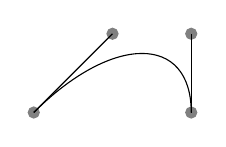
\begin{tikzpicture}
  \filldraw [gray] (0,0) circle (2pt)
  (1,1) circle (2pt)
  (2,1) circle (2pt)
  (2,0) circle (2pt);
  \draw (0,0) .. controls (1,1) and (2,1) .. (2,0);
  \draw (0,0) -- (1,1);
  \draw (2,1) -- (2,0);
\end{tikzpicture}

You can leave out the \keyword{and} (second control point), which causes the first one to be used twice.



\subsection{Circle path}
\label{sec:circle-path}

\begin{lstlisting}
\draw (0,0) circle (10pt);
\end{lstlisting}


\begin{tikzpicture}
  \draw (0,0) circle (10pt);
\end{tikzpicture}



\begin{lstlisting}
\draw (0,0) ellipse (20pt and 10pt);
\end{lstlisting}


\begin{tikzpicture}
  \draw (0,0) ellipse (20pt and 10pt);
\end{tikzpicture}

\subsection{Rectangle path}
\label{sec:rectangle-path}

\begin{lstlisting}
\filldraw [gray] (0,0) circle (2pt);
\filldraw [gray] (0.5,0.5) circle (2pt);
  \draw (0,0) rectangle (0.5,0.5);
\end{lstlisting}


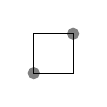
\begin{tikzpicture}
  \filldraw [gray] (0,0) circle (2pt);
  \filldraw [gray] (0.5,0.5) circle (2pt);
  \draw (0,0) rectangle (0.5,0.5);
\end{tikzpicture}

\subsection{Grid path}
\label{sec:grid-path}

\begin{lstlisting}
  \filldraw [gray] (-1.4,-1.4) circle (2pt);
  \filldraw [gray] (1.4,1.4) circle (2pt);

  \draw[step=.5cm,gray,very thin] (-1.4,-1.4) grid (1.4,1.4);
\end{lstlisting}


\begin{tikzpicture}
  \filldraw [gray] (-1.4,-1.4) circle (2pt);
  \filldraw [gray] (1.4,1.4) circle (2pt);

  \draw[step=.5cm,gray,very thin] (-1.4,-1.4) grid (1.4,1.4);
\end{tikzpicture}


\subsection{Arc path}
\label{sec:arc-path}

\begin{lstlisting}
  \filldraw [gray] (0,0) circle (2pt);
  \draw (0mm,0mm) arc (0:30:3cm);
  % (center) arc (angle1:angle2:radius)
  % an arc from angle1 to angle2 on a circle of radius

\end{lstlisting}

\begin{tikzpicture}
  \filldraw [gray] (0,0) circle (2pt);

  \draw (0mm,0mm) arc (0:30:3cm);
  % (center) arc (angle1:angle2:radius)
  % an arc from angle1 to angle2 on a circle of radius
\end{tikzpicture}



\subsection{Clipping a path}
\label{sec:clipping-path}
\begin{lstlisting}
  \draw[step=.5cm,gray,very thin] (-1.4,-1.4) grid (1.4,1.4);
  \draw (-1.5,0) -- (1.5,0);
  \draw (0,-1.5) -- (0,1.5);
  \draw (0,0) circle (1cm);
  \draw (3mm,0mm) arc (0:30:3mm);  

\end{lstlisting}

\begin{tikzpicture}
  \draw[step=.5cm,gray,very thin] (-1.4,-1.4) grid (1.4,1.4);
  \draw (-1.5,0) -- (1.5,0);
  \draw (0,-1.5) -- (0,1.5);
  \draw (0,0) circle (1cm);
  \draw (3mm,0mm) arc (0:30:3mm);  
\end{tikzpicture}

\begin{lstlisting}
  \clip (-0.1,-0.2) rectangle (1.1,0.75);
  \draw[step=.5cm,gray,very thin] (-1.4,-1.4) grid (1.4,1.4);
  \draw (-1.5,0) -- (1.5,0);
  \draw (0,-1.5) -- (0,1.5);
  \draw (0,0) circle (1cm);
  \draw (3mm,0mm) arc (0:30:3mm);  

\end{lstlisting}

\begin{tikzpicture}
  \clip (-0.1,-0.2) rectangle (1.1,0.75);
  \draw[step=.5cm,gray,very thin] (-1.4,-1.4) grid (1.4,1.4);
  \draw (-1.5,0) -- (1.5,0);
  \draw (0,-1.5) -- (0,1.5);
  \draw (0,0) circle (1cm);
  \draw (3mm,0mm) arc (0:30:3mm);  
\end{tikzpicture}

In reality, \keyword{\textbackslash{}draw} is just a shorthand for \keyword{\textbackslash{}path[draw]} and \keyword{\textbackslash{}clip} is a shorthand for \keyword{\textbackslash{}path[clip]} and you could also say \keyword{\textbackslash{}path[draw,clip]}.



\subsection{Filling}
\label{sec:filling}

\begin{lstlisting}
\fill[green!20!white] (0,0) -- (3cm,0cm) arc (0:30:3cm) -- cycle;
\end{lstlisting}

\begin{tikzpicture}
  \fill[green!20!white] (0,0) -- (3cm,0cm) arc (0:30:3cm) -- cycle;
\end{tikzpicture}


The \keyword{--cycle} causes the current path to be closed.


You can also fill and draw a path at the same time using the \keyword{\textbackslash{}filldraw} command.


\subsection{Shading}
\label{sec:shading}

\keyword{\textbackslash{}shade} and \keyword{\textbackslash{}shadedraw} are used for shading and drawing at the same time.

\begin{lstlisting}
  \shade (0,0) rectangle (2,1);
  \shade[top color=yellow,bottom color=black] (3,0) rectangle +(2,1);
  \shade[left color=yellow,right color=black] (6,0) rectangle +(2,1); % relative coordinate
  \shadedraw[inner color=yellow,outer color=black,draw=yellow] (9,0) rectangle +(2,1);
  \shade[ball color=green] (12,.5) circle (.5cm);
\end{lstlisting}

\begin{tikzpicture}
  \shade (0,0) rectangle (2,1);
  \shade[top color=yellow,bottom color=black] (3,0) rectangle +(2,1);
  \shade[left color=yellow,right color=black] (6,0) rectangle +(2,1);
  \shadedraw[inner color=yellow,outer color=black,draw=yellow] (9,0) rectangle +(2,1);
  \shade[ball color=green] (12,.5) circle (.5cm);
\end{tikzpicture}

The default shading is a smooth transition from gray to white. To specify different colors, you can use options.



\subsection{Specifying coordinates}
\label{sec:spec-coord}

\begin{itemize}
\item If you leave out the unites, the default are set to cm and for angle to degree.
\item \keyword{+} means a relative coordinate from the previous specified position and \keyword{++} means a relative coordinate from the previous specified position, making this the new specified position.
\item You can use \keyword{intersection} to specify a coordinate.
\end{itemize}


\begin{lstlisting}
\begin{tikzpicture}[scale=2]
  \draw (1,0) -- (1,1);
  \draw (0,0) -- (30:1cm);
  \filldraw [gray] (1,0) circle (2pt);
  \filldraw [gray] (intersection of 1,0--1,1 and 0,0--30:1cm) circle (2pt);
  \draw[very thick,orange] (1,0) -- (intersection of 1,0--1,1 and 0,0--30:1cm);
\end{tikzpicture}

\end{lstlisting}

\begin{tikzpicture}[scale=2]
  \draw (1,0) -- (1,1);
  \draw (0,0) -- (30:1cm);
  \filldraw [gray] (1,0) circle (2pt);
  \filldraw [gray] (intersection of 1,0--1,1 and 0,0--30:1cm) circle (2pt);
  \draw[very thick,orange] (1,0) -- (intersection of 1,0--1,1 and 0,0--30:1cm);
\end{tikzpicture}


\subsection{Adding arrow tips}
\label{sec:adding-arrow}


\begin{lstlisting}
\begin{tikzpicture}
  \draw[->] (-1.5,0) -- (1.5,0);
  \draw[<->] (-1.5,-0.5) -- (1.5,-0.5);
  \draw[<<-] (-1.5,-1) -- (1.5,-1);
\end{tikzpicture}
\end{lstlisting}

\begin{tikzpicture}
  \draw[->] (-1.5,0) -- (1.5,0);
  \draw[<->] (-1.5,-0.5) -- (1.5,-0.5);
  \draw[<<-] (-1.5,-1) -- (1.5,-1);
\end{tikzpicture}

\begin{lstlisting}
\begin{tikzpicture}[>=stealth]  % >= right arrow tip kind
  \draw[->] (-1.5,0) -- (1.5,0);
\end{tikzpicture}
\end{lstlisting}

\begin{tikzpicture}[>=stealth]  % >= right arrow tip kind
  \draw[->] (-1.5,0) -- (1.5,0);
\end{tikzpicture}



\subsection{Scoping}
\label{sec:scoping}

Scope can let you apply graphic options to a local group.

\begin{lstlisting}
\begin{tikzpicture}[ultra thick]
  \draw (0,0) -- (0,1);
  \begin{scope}[thin]
    \draw (1,0) -- (1,1);
    \draw (2,0) -- (2,1);
  \end{scope}
  \draw (3,0) -- (3,1);
\end{tikzpicture}
\end{lstlisting}

\begin{tikzpicture}[ultra thick]
  \draw (0,0) -- (0,1);
  \begin{scope}[thin]
    \draw (1,0) -- (1,1);
    \draw (2,0) -- (2,1);
  \end{scope}
  \draw (3,0) -- (3,1);
\end{tikzpicture}


\subsection{Transformations}
\label{sec:transformations}

When you specify a coordinate, TikZ applies certain transformations to the given coordinate in order to determine the finally position on the page.

\begin{lstlisting}
\begin{tikzpicture}[even odd rule,rounded corners=2pt,x=10pt,y=10pt]
  % x=10pt set the x unit to 10pt
  \filldraw (0,0)   rectangle (1,1)
  [xshift=5pt,yshift=5pt]   (0,0)   rectangle (1,1)
  [rotate=30]   (-1,-1) rectangle (2,2);

\end{tikzpicture}

\end{lstlisting}

\begin{tikzpicture}[even odd rule,rounded corners=2pt,x=10pt,y=10pt]
  % x=10pt set the x unit to 10pt
  \filldraw (0,0)   rectangle (1,1)
  [xshift=5pt,yshift=5pt]   (0,0)   rectangle (1,1)
  [rotate=30]   (-1,-1) rectangle (2,2);

\end{tikzpicture}

Options to do transformations:
\begin{itemize}
\item \keyword{xshift} and \keyword{yshift}
\item \lstinline|shift={(1,0)}| for shifting to a given point
\item \keyword{rotate} for rotating by a certain angle
\item \keyword{rotate around} for rotating around a given point
\item \keyword{scale} for scaling by a certain factor
\item \keyword{xscale} and \keyword{yscale} (\keyword{xscale=-1} is a flip)
\item \keyword{xslant} and \keyword{yslant} for slanting
\end{itemize}



\subsection{For-loops}
\label{sec:loops}
PGF introduces a command called \keyword{\textbackslash{}foreach}.
The general syntax is
\begin{lstlisting}
\foreach variable in {list of values} command
\end{lstlisting}

\begin{lstlisting}
\begin{tikzpicture}
  \foreach \x in {1,2,...,5,7,9,...,12}
    \foreach \y in {1,...,5}
    {
      \draw (\x,\y) +(-.5,-.5) rectangle ++(.5,.5);
    }
\end{tikzpicture}

\end{lstlisting}

\begin{tikzpicture}
  \foreach \x in {1,2,...,5,7,9,...,12}
    \foreach \y in {1,...,5}
    {
      \draw (\x,\y) +(-.5,-.5) rectangle ++(.5,.5);
    }
\end{tikzpicture}

If you provide two numbers before the \keyword{...}, the \keyword{\textbackslash{}foreach} statement will use their difference for the stepping.




\begin{tikzpicture}
  \foreach \x\y in {0/5,1/2,2/9,3/22,4/31,5/6}
  {
    \node [rectangle,draw,minimum size=1cm] () at (\x ,0) {\y};
  }
\end{tikzpicture}

\begin{lstlisting}

\begin{tikzpicture}
  \foreach \x\y in {0/5,1/2,2/9,3/22,4/31,5/6}
  {
    \node [rectangle,draw,minimum size=1cm] () at (\x ,0) {\y};
  }
\end{tikzpicture}
\end{lstlisting}
\subsection{Adding text}
\label{sec:adding-text}

\begin{lstlisting}
\begin{tikzpicture}
  \draw (0,0) -- node[above=1pt] {above=1pt} (3,0)
  (0,-1) -- node[anchor=north] {anchor=north} (3,-1);
  \draw (0,-3) .. controls (6,-2) and (9,-2) ..
  node[near start,sloped,above] {near start}
  node {midway}
  node[very near end,sloped,below] {very near end} (12,-3);
\end{tikzpicture}
\end{lstlisting}


\begin{tikzpicture}
  \draw (0,0) -- node[above=1pt] {above=1pt} (3,0)
  (0,-1) -- node[anchor=north] {anchor=north} (3,-1);
  \draw (0,-3) .. controls (6,-2) and (9,-2) ..
  node[near start,sloped,above] {near start}
  node {midway}
  node[very near end,sloped,below] {very near end} (12,-3);
\end{tikzpicture}

When TikZ is constructing a path and encounters the keyword \keyword{node} in the middle of a path, it reads a ``node specification''.
The keyword \keyword{node} is typically followed by some options and then some text between curly braces.
This text is put inside a normal TEX box.
All nodes are drawn only after the path has been completely drawn.
You can determine the direction to the position with the \keyword{anchor} option.
And there are simplified writing for the \keyword{anchor} option.
\keyword{below} does the same as \keyword{anchor=south east}.
You can also position labels on curves and, by adding the \keyword{sloped} option, have them rotated such that they match the line’s slope.

\subsection{Load library packages}
\label{sec:load-libr-pack}

\begin{lstlisting}
\usetikzlibrary{arrows,snakes,backgrounds}
\end{lstlisting}




\subsection{Set style}
\label{sec:set-style}

For some commonly used setting, you can set a short name for this setting to save typing and improve clarity.
\begin{lstlisting}
\tikzstyle{place}=[circle,draw=blue!50,fill=blue!20,thick, inner sep=0pt,minimum size=6mm]

\begin{tikzpicture}
  \node [place]  (waiting 1) at (0,2) {};
\end{tikzpicture}
\end{lstlisting}


\subsection{Set color}
\label{sec:set-color}

\begin{lstlisting}
\colorlet{anglecolor}{green!50!black}
\colorlet{sincolor}{red}

\filldraw[fill=green!20,draw=anglecolor] (0,0) -- (3mm,0pt) arc(0:30:3mm);
\end{lstlisting}


\subsection{Local definition}
\label{sec:local-definition}

\begin{lstlisting}
\def\costhirty{0.8660256}
\end{lstlisting}
\subsection{Node}
\label{sec:node}



A node have a \argument{position} and can have a \argument{shape} and \argument{name}.


The \funcword{\textbackslash{}node} command is an abbreviation for \funcword{\textbackslash{}path node}.

\begin{lstlisting}
% shape (circle), style (blue!50,fill=blue!20,thick), size (inner sep=0pt,minimum size=6mm)
\tikzstyle{place}=[circle,draw=blue!50,fill=blue!20,thick,
                   inner sep=0pt,minimum size=6mm]
\tikzstyle{transition}=[rectangle,draw=black!50,fill=black!20,thick,
                        inner sep=0pt,minimum size=4mm]
\begin{tikzpicture}
  % option   name   coordinate  text
  \node[place]      (waiting 1)      at ( 0,2) {};
  \node[place]      (critical 1)     at ( 0,1) {};
  \node[place]      (semaphore)      at ( 0,0) {};
  \node[transition] (leave critical) at ( 1,1) {};
  \node[transition] (enter critical) at (-1,1) {};
\end{tikzpicture}
\end{lstlisting}



% shape (circle), style (blue!50,fill=blue!20,thick), size (inner sep=0pt,minimum size=6mm)
\tikzstyle{place}=[circle,draw=blue!50,fill=blue!20,thick,
                   inner sep=0pt,minimum size=6mm]
\tikzstyle{transition}=[rectangle,draw=black!50,fill=black!20,thick,
                        inner sep=0pt,minimum size=4mm]
\begin{tikzpicture}
  % option   name   coordinate  text
  \node[place]      (waiting 1)      at ( 0,2) {};
  \node[place]      (critical 1)     at ( 0,1) {};
  \node[place]      (semaphore)      at ( 0,0) {};
  \node[transition] (leave critical) at ( 1,1) {};
  \node[transition] (enter critical) at (-1,1) {};
\end{tikzpicture}





We can use relative coordinates and add label to a node.
\begin{lstlisting}
\begin{tikzpicture}
  \tikzstyle{every label}=[red]
  \node[place]   (waiting)      {};                      
  \node[place]   (critical)     [below of=waiting]  {};  
  \node[place]   (semaphore)    [below of=critical,      
                                label=above:$s\le3$] {};   

  \node[transition] (leave critical) [right of=critical] {};
  \node[transition] (enter critical) [left of=critical]  {};
\end{tikzpicture}
\end{lstlisting}


\begin{tikzpicture}
  \tikzstyle{every label}=[red]
  \node[place]   (waiting)      {};                      
  \node[place]   (critical)     [below of=waiting]  {};  
  \node[place]   (semaphore)    [below of=critical,      
                                label=above:$s\le3$] {};   

  \node[transition] (leave critical) [right of=critical] {};
  \node[transition] (enter critical) [left of=critical]  {};
\end{tikzpicture}


We can use \keyword{edge} to draw connection lines.
\begin{lstlisting}
\tikzstyle{pre}=[<-,shorten <=1pt,>=stealth,semithick]
\tikzstyle{post}=[->,shorten >=1pt,>=stealth,semithick]
\begin{tikzpicture}[bend angle=45]
  \node[place]    (waiting)                            {};
  \node[place]    (critical)       [below of=waiting]  {};
  \node[place]    (semaphore)      [below of=critical] {};

  \node[transition] (leave critical) [right of=critical] {}
  edge [pre]                                 (critical)
  edge [post,bend right] node[auto,swap] {2} (waiting)
  edge [pre, bend left]                      (semaphore);
  \node[transition] (enter critical) [left of=critical]  {}
  edge [post]                              (critical) 
  edge [pre, bend left]                    (waiting)
  edge [post,bend right]                   (semaphore);
\end{tikzpicture}
\end{lstlisting}

\tikzstyle{pre}=[<-,shorten <=1pt,>=stealth,semithick]
\tikzstyle{post}=[->,shorten >=1pt,>=stealth,semithick]
\begin{tikzpicture}[bend angle=45]
  \node[place]    (waiting)                            {};
  \node[place]    (critical)       [below of=waiting]  {};
  \node[place]    (semaphore)      [below of=critical] {};

  \node[transition] (leave critical) [right of=critical] {}
  edge [pre]                                 (critical)
  edge [post,bend right] node[auto,swap] {2} (waiting)
  edge [pre, bend left]                      (semaphore);
  \node[transition] (enter critical) [left of=critical]  {}
  edge [post]                              (critical) 
  edge [pre, bend left]                    (waiting)
  edge [post,bend right]                   (semaphore);
\end{tikzpicture}



\subsection{Snake line}
\label{sec:snake-line}
\usetikzlibrary{snakes}
\begin{tikzpicture}
  \draw [->,snake=snake,
         segment amplitude=.4mm,
         segment length=2mm,
         line after snake=1mm] (0,0) -- (3,0);
\end{tikzpicture}


\begin{lstlisting}

\begin{tikzpicture}
  \draw [->,snake=snake,
         segment amplitude=.4mm,
         segment length=2mm,
         line after snake=1mm] (0,0) -- (3,0);
\end{tikzpicture}
\end{lstlisting}
\section{Examples}
\label{sec:examples}

\subsection{A picture for Karl’s students}
\label{sec:pict-karls-stud}

\begin{tikzpicture}[scale=3,cap=round]
  % Local definitions
  \def\costhirty{0.8660256}
  % Colors
  \colorlet{anglecolor}{green!50!black}
  \colorlet{sincolor}{red}
  \colorlet{tancolor}{orange!80!black}
  \colorlet{coscolor}{blue}
  % Styles
  \tikzstyle{axes}=[]
  \tikzstyle{important line}=[very thick]
  \tikzstyle{information text}=[rounded corners,fill=red!10,inner sep=1ex]
  % The graphic
  \draw[style=help lines,step=0.5cm] (-1.4,-1.4) grid (1.4,1.4);
  \draw (0,0) circle (1cm);
  \begin{scope}[style=axes]
    \draw[->] (-1.5,0) -- (1.5,0) node[right] {$x$} coordinate(x axis);
    \draw[->] (0,-1.5) -- (0,1.5) node[above] {$y$} coordinate(y axis);
    \foreach \x/\xtext in {-1, -.5/-\frac{1}{2}, 1}
    \draw[xshift=\x cm] (0pt,1pt) -- (0pt,-1pt) node[below,fill=white] {$\xtext$};
    \foreach \y/\ytext in {-1, -.5/-\frac{1}{2}, .5/\frac{1}{2}, 1}
    \draw[yshift=\y cm] (1pt,0pt) -- (-1pt,0pt) node[left,fill=white] {$\ytext$};
  \end{scope}
  \filldraw[fill=green!20,draw=anglecolor] (0,0) -- (3mm,0pt) arc(0:30:3mm);
  \draw (15:2mm) node[anglecolor] {$\alpha$};
  \draw[style=important line,sincolor]
  (30:1cm) -- node[left=1pt,fill=white] {$\sin \alpha$} (30:1cm |- x axis);
  \draw[style=important line,coscolor]
  (30:1cm |- x axis) -- node[below=2pt,fill=white] {$\cos \alpha$} (0,0);
  \draw[style=important line,tancolor] (1,0) -- node[right=1pt,fill=white] {
    $\displaystyle \tan \alpha \color{black}=
    \frac{{\color{sincolor}\sin \alpha}}{\color{coscolor}\cos \alpha}$}
  (intersection of 0,0--30:1cm and 1,0--1,1) coordinate (t);
  \draw (0,0) -- (t);
  \draw[xshift=1.85cm]
  node[right,text width=6cm,style=information text]
  {
    The {\color{anglecolor} angle $\alpha$} is $30^\circ$ in the
      example ($\pi/6$ in radians). The {\color{sincolor}sine of
        $\alpha$}, which is the height of the red line, is
      \[
      {\color{sincolor} \sin \alpha} = 1/2.
      \]

      By the Theorem of Pythagoras we have ${\color{coscolor}\cos ^2 \alpha}+{\color{sincolor} \sin^{2} \alpha} = 1/alpha=1$.
      Thus the length of the blue line, which is the {\color{coscolor} cosine of $\alpha$}, must be
    $$
    {\color{coscolor}\cos \alpha}=\sqrt{1-1 / 4}=\frac{1}{2} \sqrt{3}
    $$
    This shows that {\color{tancolor}$\tan \alpha$}, which is the height of the orange line, is
    $$
    {\color{tancolor}\tan \alpha}=\frac{\color{sincolor}\sin \alpha}{\color{coscolor}\cos \alpha}=1 / \sqrt{3}
    $$
  };
\end{tikzpicture}

\begin{lstlisting}
\begin{tikzpicture}[scale=3,cap=round]
% Local definitions
  \def\costhirty{0.8660256}
% Colors
  \colorlet{anglecolor}{green!50!black}
  \colorlet{sincolor}{red}
  \colorlet{tancolor}{orange!80!black}
  \colorlet{coscolor}{blue}
% Styles
  \tikzstyle{axes}=[]
  \tikzstyle{important line}=[very thick]
  \tikzstyle{information text}=[rounded corners,fill=red!10,inner sep=1ex]
% The graphic
  \draw[style=help lines,step=0.5cm] (-1.4,-1.4) grid (1.4,1.4);
  \draw (0,0) circle (1cm);
  \begin{scope}[style=axes]
    \draw[->] (-1.5,0) -- (1.5,0) node[right] {$x$} coordinate(x axis);
    \draw[->] (0,-1.5) -- (0,1.5) node[above] {$y$} coordinate(y axis);
    \foreach \x/\xtext in {-1, -.5/-\frac{1}{2}, 1}
      \draw[xshift=\x cm] (0pt,1pt) -- (0pt,-1pt) node[below,fill=white] {$\xtext$};
    \foreach \y/\ytext in {-1, -.5/-\frac{1}{2}, .5/\frac{1}{2}, 1}
      \draw[yshift=\y cm] (1pt,0pt) -- (-1pt,0pt) node[left,fill=white] {$\ytext$};
\end{scope}
  \filldraw[fill=green!20,draw=anglecolor] (0,0) -- (3mm,0pt) arc(0:30:3mm);
  \draw (15:2mm) node[anglecolor] {$\alpha$};
  \draw[style=important line,sincolor]
    (30:1cm) -- node[left=1pt,fill=white] {$\sin \alpha$} (30:1cm |- x axis);
  \draw[style=important line,coscolor]
    (30:1cm |- x axis) -- node[below=2pt,fill=white] {$\cos \alpha$} (0,0);
  \draw[style=important line,tancolor] (1,0) -- node[right=1pt,fill=white] {
    $\displaystyle \tan \alpha \color{black}=
    \frac{{\color{sincolor}\sin \alpha}}{\color{coscolor}\cos \alpha}$}
    (intersection of 0,0--30:1cm and 1,0--1,1) coordinate (t);
  \draw (0,0) -- (t);
  \draw[xshift=1.85cm]
    node[right,text width=6cm,style=information text]
    {
      The {\color{anglecolor} angle $\alpha$} is $30^\circ$ in the
      example ($\pi/6$ in radians). The {\color{sincolor}sine of
        $\alpha$}, which is the height of the red line, is
      \[
      {\color{sincolor} \sin \alpha} = 1/2.
      \]
      By the Theorem of Pythagoras ...
    };
\end{tikzpicture}
\end{lstlisting}



\subsection{A Petri-Net for Hagen}
\label{sec:petri-net-hagen}

\usetikzlibrary{arrows,snakes,backgrounds}

\tikzstyle{place}=[circle,draw=blue!50,fill=blue!20,thick,inner sep=0pt,minimum size=6mm]
\tikzstyle{transition}=[rectangle,draw=black!50,fill=black!20,thick,inner sep=0pt,minimum size=4mm]

\tikzstyle{pre}=[<-,shorten <=1pt,>=stealth,semithick]
\tikzstyle{post}=[->,shorten >=1pt,>=stealth,semithick]

\tikzstyle{every place}=[minimum size=6cm,thick,draw=blue!75,fill=blue!20]
\tikzstyle{every transition}=[thick,draw=black!75,fill=black!20]
\tikzstyle{red place}=[place,draw=red!75,fill=red!20]
\tikzstyle{every label}=[red]


\begin{tikzpicture}[node distance=1.3cm,>=stealth,bend angle=45,auto]
  \node [place] (w1)  {};
  \node [place] (c1) [below of=w1] {};
  \node [place] (s) [below of=c1,label=above:\(s\le 3\)] {};
  \node [place] (c2) [below of=s] {};
  \node [place] (w2) [below of=c2] {};

  \node [transition] (e1) [left of=c1] {}
  edge [pre,bend left] (w1)
  edge [post,bend right] (s)
  edge [post] (c1);
  \node [transition] (e2) [left of=c2] {}
  edge [pre, bend right] (w2)
  edge [pre, bend left] (s)
  edge [post] (c2);
  \node [transition] (l1) [right of=c1] {}
  edge [pre] (c1)
  edge [pre,bend left] (s)
  edge [post,bend right] node [swap] {2} (w1);
  \node [transition] (l2) [right of=c2] {}
  edge [pre] (c2)
  edge [pre,bend right] (s)
  edge [post,bend left] node {2} (w2);

  \begin{scope}[xshift=6cm]
    \node [place] (w1') {};
    \node [place] (c1') [below of=w1'] {};
    \node [red place] (s1') [below of=c1',xshift=-0.5cm] [label=left:\(s\)] {};
    \node [red place] (s2') [below of=c1',xshift=0.5cm] [label=right:\(\bar s\)] {};
    \node [place] (c2') [below of=s1',xshift=.5cm] {};
    \node [place] (w2') [below of=c2'] {};

    \node [transition] (e1') [left of=c1'] {}
    edge [pre,bend left] (w1')
    edge [post] (s1')
    edge [pre] (s2')
    edge [post] (c1');
    \node [transition] (e2') [left of=c2'] {}
    edge [pre,bend right] (w2')
    edge [post] (s1')
    edge [pre] (s2')
    edge [post] (c2');
    \node [transition] (l1') [right of=c1'] {}
    edge [pre] (c1')
    edge [pre] (s1')
    edge [post] (s2')
    edge [post,bend right] node [swap]  {2} (w1');
    \node [transition] (l2') [right of=c2'] {}
    edge [pre] (c2')
    edge [pre] (s1')
    edge [post] (s2')
    edge [post,bend left] node {2} (w2');
  \end{scope}

  \draw [-to,thick,snake=snake,segment amplitude=.4mm,segment length=2mm,line after snake=1mm]
    ([xshift=5mm]s -| l1) -- ([xshift=-5mm]s1' -| e1')
    node [above=1mm,midway,text width=3cm,text centered]
      {replacement of the \textcolor{red}{capacity} by \textcolor{red}{two places}};
  \begin{pgfonlayer}{background}
    \filldraw [line width=4mm,join=round,black!10]
      (w1.north  -| l1.east)  rectangle (w2.south  -| e1.west)
      (w1'.north -| l1'.east) rectangle (w2'.south -| e1'.west);
  \end{pgfonlayer}
\end{tikzpicture}


\begin{lstlisting}
\usetikzlibrary{arrows,snakes,backgrounds}

\tikzstyle{place}=[circle,draw=blue!50,fill=blue!20,thick,inner sep=0pt,minimum size=6mm]
\tikzstyle{transition}=[rectangle,draw=black!50,fill=black!20,thick,inner sep=0pt,minimum size=4mm]

\tikzstyle{pre}=[<-,shorten <=1pt,>=stealth,semithick]
\tikzstyle{post}=[->,shorten >=1pt,>=stealth,semithick]

\tikzstyle{every place}=[minimum size=6cm,thick,draw=blue!75,fill=blue!20]
\tikzstyle{every transition}=[thick,draw=black!75,fill=black!20]
\tikzstyle{red place}=[place,draw=red!75,fill=red!20]
\tikzstyle{every label}=[red]


\begin{tikzpicture}[node distance=1.3cm,>=stealth,bend angle=45,auto]
  \node [place] (w1)  {};
  \node [place] (c1) [below of=w1] {};
  \node [place] (s) [below of=c1,label=above:\(s\le 3\)] {};
  \node [place] (c2) [below of=s] {};
  \node [place] (w2) [below of=c2] {};

  \node [transition] (e1) [left of=c1] {}
  edge [pre,bend left] (w1)
  edge [post,bend right] (s)
  edge [post] (c1);
  \node [transition] (e2) [left of=c2] {}
  edge [pre, bend right] (w2)
  edge [pre, bend left] (s)
  edge [post] (c2);
  \node [transition] (l1) [right of=c1] {}
  edge [pre] (c1)
  edge [pre,bend left] (s)
  edge [post,bend right] node [swap] {2} (w1);
  \node [transition] (l2) [right of=c2] {}
  edge [pre] (c2)
  edge [pre,bend right] (s)
  edge [post,bend left] node {2} (w2);

  \begin{scope}[xshift=6cm]
    \node [place] (w1') {};
    \node [place] (c1') [below of=w1'] {};
    \node [red place] (s1') [below of=c1',xshift=-0.5cm] [label=left:\(s\)] {};
    \node [red place] (s2') [below of=c1',xshift=0.5cm] [label=right:\(\bar s\)] {};
    \node [place] (c2') [below of=s1',xshift=.5cm] {};
    \node [place] (w2') [below of=c2'] {};

    \node [transition] (e1') [left of=c1'] {}
    edge [pre,bend left] (w1')
    edge [post] (s1')
    edge [pre] (s2')
    edge [post] (c1');
    \node [transition] (e2') [left of=c2'] {}
    edge [pre,bend right] (w2')
    edge [post] (s1')
    edge [pre] (s2')
    edge [post] (c2');
    \node [transition] (l1') [right of=c1'] {}
    edge [pre] (c1')
    edge [pre] (s1')
    edge [post] (s2')
    edge [post,bend right] node [swap]  {2} (w1');
    \node [transition] (l2') [right of=c2'] {}
    edge [pre] (c2')
    edge [pre] (s1')
    edge [post] (s2')
    edge [post,bend left] node {2} (w2');
  \end{scope}

  \draw [-to,thick,snake=snake,segment amplitude=.4mm,segment length=2mm,line after snake=1mm]
    ([xshift=5mm]s -| l1) -- ([xshift=-5mm]s1' -| e1')
    node [above=1mm,midway,text width=3cm,text centered]
      {replacement of the \textcolor{red}{capacity} by \textcolor{red}{two places}};
  \begin{pgfonlayer}{background}
    \filldraw [line width=4mm,join=round,black!10]
      (w1.north  -| l1.east)  rectangle (w2.south  -| e1.west)
      (w1'.north -| l1'.east) rectangle (w2'.south -| e1'.west);
  \end{pgfonlayer}
\end{tikzpicture}

\end{lstlisting}
%%% Local Variables:
%%% mode: latex
%%% TeX-master: "latex"
%%% End:


\chapter{Reference}
\label{cha:reference}

\begin{lstlisting}
% \usepackage{amssymb}
\checkmark{}
\end{lstlisting}
\checkmark{}
%%% Local Variables:
%%% mode: latex
%%% TeX-master: "latex"
%%% End:



% Pages are numbered with Arabic numbers.
% Chapters generate a table of contents entry but don't get a number.
\backmatter
\nocite{*}
\bibliographystyle{alpha}
\bibliography{tex}

\clearpage{}
% just setting an anchor like \hypertarget{}{}
% fix the problem that anchor point to the previous section
\phantomsection                 
\printindex{}
\end{document}

%%% Local Variables:
%%% mode: latex
%%% TeX-master: t
%%% End:

